\documentclass{article}
\usepackage{graphicx,fullpage,lscape,amssymb,amsmath,xtab,setspace}
\usepackage{hyperref}
\author{Pieter Vermeesch\\
{\small Department of Geological and Environmental Sciences, 
Stanford University}}
\date{}
\title{Tectonic discrimination diagrams revisited}
\begin{document}

\onehalfspace
\maketitle

\begin{center}
{\it Geochemistry, Geophysics, Geosystems} (G$^3$) manuscript 2005gc001092
\end{center}

\begin{abstract}
The decision  boundaries of most tectonic  discrimination diagrams are
drawn by eye.  Discriminant  analysis is a statistically more rigorous
way to  determine the  tectonic affinity of  oceanic basalts  based on
their bulk-rock chemistry.   This method was applied to  a database of
756  oceanic  basalts  of   known  tectonic  affinity  (ocean  island,
mid-ocean ridge, or  island arc). For each of  these training data, up
to  45 major, minor  and trace  elements were  measured.  Discriminant
analysis  assumes  multivariate  normality.   If the  same  covariance
structure is  shared by all  the classes (i.e.,  tectonic affinities),
the decision boundaries are linear, hence the term linear discriminant
analysis  (LDA).   In   contrast  with  this,  quadratic  discriminant
analysis  (QDA)  allows  the  classes  to  have  different  covariance
structures.   To solve  the statistical  problems associated  with the
constant-sum constraint of geochemical data, the training data must be
transformed  to  log-ratio  space  before  performing  a  discriminant
analysis.  The  results can be  mapped back to the  compositional data
space  using  the  inverse  log-ratio transformation.   An  exhaustive
exploration of 14,190  possible ternary discrimination diagrams yields
the Ti-Si-Sr system as the best linear, and the Na-Nb-Sr system as the
best quadratic discrimination diagram.   The best linear and quadratic
discrimination diagrams  using only immobile elements  are Ti-V-Sc and
Ti-V-Sm,  respectively.  As  little as  5\% of  the training  data are
misclassified  by these  discrimination  diagrams. Testing  them on  a
second database of 182 samples that were not part of the training data
yields a  more reliable estimate of future  performance.  Although QDA
misclassifies fewer training data  than LDA, the opposite is generally
true for the  test data.  Therefore, LDA is a  cruder, but more robust
classifier than QDA.   Another advantage of LDA is  that it provides a
powerful  way  to  reduce   the  dimensionality  of  the  multivariate
geochemical  data in a  similar way  to principal  component analysis.
This procedure  yields a  small number of  ``discriminant functions'',
which are linear combinations  of the original variables that maximize
the between-class variance relative to the within-class variance.
\end{abstract}

\section{Introduction}

Recovering the tectonic affinity of ancient ophiolites is a problem of
great  scientific  interest.   In   addition  to  field  data,  basalt
geochemistry  is  another  way  to  address  this  problem.   Tectonic
discrimination diagrams  have been a popular technique  for doing this
since the  publication of  landmark papers by  Pearce and  Cann (1971,
1973). This paper revisits some of the popular discrimination diagrams
that have been in use  since then.  Nearly all discrimination diagrams
that  are  currently in  use  were drawn  by  eye.  The present  paper
revisits these diagrams in a statistically more rigorous way.\\

First, a short introduction will be given to the discriminant analysis
method.    The  fundamental  difference   between  the   reduction  in
dimensionality  achieved   by  principal  components   and  by  linear
discriminant analysis  will be  explained.  Then, the  consequences of
the  constant-sum  constraint  of  geochemical data  for  discriminant
analysis   will  be   discussed.    In  Section   \ref{sec:aitchison},
Aitchison's  (1982, 1986)  solution to  this problem  will  be briefly
explained.    Section   \ref{sec:revisit}   revisits   some   of   the
historically most important and popular discrimination diagrams, based
on a new database of  oceanic basalts of known tectonic affinity.  The
effect of data-closure will be  taken into account and a statistically
rigorous  re-evaluation of  these diagrams  will be  made in  both the
linear and the quadratic case.\\

This paper does not restrict itself to only those geochemical features
that   have  already   been   used  by   previous  workers.    Section
\ref{sec:exhaustive} gives  an exhaustive exploration  of all possible
bivariate and ternary discrimination diagrams using a set of 45 major,
minor, and trace elements. This will  result in a list of the 100 best
linear and quadratic ternary discriminators, ranked according to their
success   in  classifying   the  training   data.    Finally,  Section
\ref{sec:test}  tests  the   most  important  discrimination  diagrams
discussed  elsewhere in  the paper  on  a second  database of  oceanic
basalts that were not part of  the training data. This provides a more
objective estimator of misclassification  risk on future data than the
misclassification rate  of the training  data.  Section \ref{sec:test}
also contains a formal comparison  of the new decision boundaries with
the  old ones  of Pearce  and Cann  (1973), Shervais  (1982), Meschede
(1986) and  Wood  (1980). It  will  be  shown  that the  new  decision
boundaries perform at least as well as the old ones.

\section{Discriminant analysis} \label{sec:discriminant}

Consider a  dataset of a large  number of N-dimensional  data X, which
belong  to one  of  K  classes.  For  example,  X might  be  a set  of
geochemical data (e.g.,  SiO$_2$, Al$_2$O$_3$,etc) from basaltic rocks
of K tectonic affinities (e.g.,  mid ocean ridge, ocean island, island
arc,...). We  might ask  ourselves which of  these classes  an unknown
sample x belongs to.  This  question is answered by {\it Bayes' Rule}:
the decision d  is the class G (1$\leq$G$\leq$K)  that has the highest
{\it posterior probability} given the data x:

\begin{equation}
  \label{eq:bayesRule}
  d = \underset{k=1,...,K}{argmax} ~ Pr(G=k|X=x)
\end{equation}

where {\it argmax}  stands for ``argument of the  maximum'', i.e. when
f(k) reaches  a maximum when  k=d, then $\underset{k=1,...,K}{argmax}$
f(k) = d.  This posterior  distribution can be calculated according to
Bayes' Theorem:

\begin{equation}
  \label{eq:bayesTheorem}
  Pr(G|X) \propto Pr(X|G)Pr(G)
\end{equation}

where  Pr(X$|$G) is the  {\it probability  density} of  the data  in a
given class, and Pr(G) the {\it prior probability} of the class, which
we  will consider  uniformly distributed  (i.e., Pr(G=1)  =  Pr(G=2) =
... = Pr(G=K)  = 1/K) in this paper.   Therefore, plugging Equation
\ref{eq:bayesTheorem}  into Equation  \ref{eq:bayesRule} reduces  Bayes' Rule
to a comparison of probability density estimates.  We now make
the simplifying assumption of multivariate normality:

\begin{equation}
  \label{eq:multiNorm}
  Pr(X=x|G=k) = \frac{exp \left( -\frac{1}{2}(x-\mu_k)^T\Sigma_k^{-1}(x-\mu_k) \right)}
                 {(2\pi)^{N/2}\sqrt{|\Sigma_k|}}
\end{equation}

Where  $\mu_k$ and  $\Sigma_k$  are  the mean  and  covariance of  the
k$^{th}$ class and (x-$\mu_k)^T$ indicates the transpose of the matrix
(x-$\mu_k$).    Using    Equation   \ref{eq:multiNorm},   and   taking
logarithms, Equation \ref{eq:bayesRule} becomes:

\begin{equation}
  \label{eq:quadRule}
d = \underset{k=1,...,K}{argmax} ~ -\frac{1}{2}log|\Sigma_k| -
                            \frac{1}{2}(x-\mu_k)^T\Sigma_k^{-1}(x-\mu_k)
\end{equation}

Equation   \ref{eq:quadRule}   is  the   basis   for  {\it   quadratic
discriminant analysis} (QDA). Usually,  $\mu_k$ and $\Sigma_k$ are not
known, and must  be estimated from the training data.   If we make the
additional assumption  that all the classes share  the same covariance
structure  (i.e., $\Sigma_k$  = $\Sigma$  $\forall$ k),  then Equation
\ref{eq:bayesRule} simplifies to:

\begin{equation}
  \label{eq:linRule}
d = \underset{k=1,...,K}{argmax} ~ x^T\Sigma^{-1}\mu_k-\frac{1}{2}\mu_k^T\Sigma^{-1}\mu_k
\end{equation}

This is the  basis of {\it linear discriminant  analysis} (LDA), which
has  some   desirable  properties.   For   example,  because  Equation
\ref{eq:linRule} is  linear in x, the decision  boundaries between the
different  classes  are  straight  lines  (Figure  \ref{fig:linDisc}).
Furthermore,   LDA   can   lead   to  a   significant   reduction   in
dimensionality, in a similar way to {\it principal component analysis}
(PCA).  PCA  finds an orthogonal  transformation B (i.e.,  a rotation)
that transforms  the centered data  (X) to orthogonality, so  that the
elements of the vector BX are uncorrelated.  B can be calculated by an
eigenvalue  decomposition  of  the  covariance matrix  $\Sigma$.   The
eigenvectors  are  orthogonal  linear  combinations  of  the  original
variables, and  the eigenvalues give  their variances.  The  first few
principal components generally account  for most of the variability of
the  data,  constituting  a  significant reduction  of  dimensionality
(Figure \ref{fig:PCAvsLDA}).\\

Like  PCA,  LDA  also   finds  linear  combinations  of  the  original
variables.  However, this time, we do not want to maximize the overall
variability,  but  find the  orthogonal  transformation  Z  = BX  that
maximizes the {\it between class}  variance S$_b$ relative to the {\it
within class} variance S$_w$, where S$_b$ is the variance of the class
means of Z,  and S$_w$ is the pooled variance  about the means (Figure
\ref{fig:PCAvsLDA}).

\section{The compositional data problem} \label{sec:compositionalProblems}

One of the  assumptions of discriminant analysis is  that the elements
of X are  statistically {\it independent} from each  other, apart from
the  covariance structure contained  in their  multivariate normality.
However, geochemical data are generally  expressed as parts of a whole
(percent or  ppm) and, therefore,  are not free to  vary independently
from   each  other.    For  example,   in  a   three-component  system
(A+B+C=100\%), increasing one component (e.g., A) causes a decrease in
the two other  components (B and C).  The  constant-sum constraint has
several  consequences,  besides   introducing  a  negative  bias  into
correlations between  components.  One  of these consequences  is that
the  arithmetic mean  of compositional  data has  no  physical meaning
(Figure  \ref{fig:closure}).  This  is very  unfortunate  because some
popular  discrimination diagrams  (e.g.,  Pearce and  Cann, 1973)  are
based on  the arithmetic  means of multiple  samples, and it  is these
averages  that  are  published  in  the  literature.   Therefore,  the
discriminant analyses  discussed in  this paper will  not be  based on
these historic  datasets, but  will use a  newly compiled  database of
individual analyses.\\



Another  statistical  issue that  deserves  to  be  mentioned is  {\it
spurious  correlation}.  Bivariate  plots of  the form  X vs.   X/Y, X
vs. Y/X or X/Z vs. Y/Z  can show some degree of correlation, even when
X,  Y  and  Z  are  completely independent  from  each  other  (Figure
\ref{fig:spurious}).   This effect  was  first discussed  more than  a
century ago  by Pearson  (1897), and was  brought to the  attention of
geologists more  than half a  century ago by Chayes  (1949).  Spurious
correlation  is  an   effect  that  should  be  borne   in  mind  when
interpreting  discrimination  diagrams   like  the  Zr/Y-Ti/Y  diagram
(Pearce and Gale, 1977), the Zr/Y-Zr diagram (Pearce and Norry, 1979),
or  the Ti/Y-Nb/Y  and K$_2$O/Yb-Ta/Yb  diagrams (Pearce,  1982). Note
that whereas in  Figure \ref{fig:spurious}, X, Y and  Z are completely
independent, this is never the case for compositional data, due to the
constant-sum  constraint described before.   This only  aggravates the
problem of spurious correlation.

\section{Aitchison's solution to the compositional data problem}
\label{sec:aitchison}

Although Chayes  (1949, 1960, 1971) made  significant contributions to
the  compositional data  problem, the  real breakthrough  was  made by
Aitchison  (1982,   1986).   Aitchison  argues   that  N-variate  data
constrained to a constant sum  form an N-1 dimensional sample space or
{\it simplex}. An example of a  simplex for N=3 is the ternary diagram
(e.g.,  Weltje, 2002).   The very  fact that  it is  possible  to plot
ternary data  on a  two-dimensional sheet of  paper tells us  that the
sample  space really  has only  two,  and not  three dimensions.   The
``traditional'' statistics of real space ($\mathbb{R}^N$) do no longer
work      on      the      simplex      ($\Delta_{N-1}$).       Figure
\ref{fig:closure_ternary_wrong} shows the breakdown of the calculation
of 100(1-$\alpha$)\%  confidence intervals on  $\Delta_{2}$.  Treating
$\Delta_{2}$  the same  way as  $\mathbb{R}^3$ yields  95\% confidence
polygons that  partly fall outside the  ternary diagram, corresponding
to meaningless negative values of x, y and z.\\

As a  solution to this  problem, Aitchison suggested to  transform the
data  from   $\Delta_{N-1}$  to  $\mathbb{R}^{N-1}$   using  the  {\it
log-ratio  transformation} (Figure  \ref{fig:closure_mapping}).  After
performing the  desired (``traditional'') statistical  analysis on the
transformed  data  in  $\mathbb{R}^{N-1}$,  the results  can  then  be
transformed  back  to   $\Delta_{N-1}$  using  the  inverse  log-ratio
transformation. For example, in the ternary system (X+Y+Z=1), we could
use  the   transformed  values  V   =  log(X/Z)  and  W   =  log(Y/Z).
Alternatively,  we  could  also  use  V=log(X/Y)  and  W=log(Z/Y),  or
V=log(Y/X)  and W=log(Z/X).  The  inverse log-ratio  transformation is
given by:

\begin{equation}
  \label{eq:inverse_transform}
  X  =  \frac{e^V}{e^V+e^W+1},~\\
  Y  =  \frac{e^W}{e^V+e^W+1},~\\
  Z  =  \frac{1}{e^V+e^W+1}
\end{equation}

The     back-transformed      confidence     regions     of     Figure
\ref{fig:closure_mapping}  are no  longer  elliptical, but  completely
fall   within   the  ternary   diagram,   as   they  should.    Figure
\ref{fig:closure_discriminant_wrong}  shows an  LDA  of the  synthetic
data      of      Figures     \ref{fig:closure_ternary_wrong}      and
\ref{fig:closure_mapping}, done the  ``wrong'' way (i.e., treating the
simplex  as a  regular  data  space).  As  explained  in the  previous
section, such  an analysis yields linear decision  boundaries. 10\% of
the      training      data      were      misclassified.       Figure
\ref{fig:closure_binary_discriminant_right}  shows  an  LDA  done  the
``correct'' way (i.e., after mapping the data to log-ratio space). The
decision boundaries are still linear, but this time only $\sim$ 3\% of
the training  data were  misclassified. Because log(Y/Z)  and log(X/Z)
are rather hard quantities to interpret,  it is a good idea to map the
results  back  to the  ternary  diagram  using  the inverse  log-ratio
transformation  (Figure \ref{fig:closure_ternary_discriminant_right}).
The transformed decision boundaries  are no longer linear, but curved.
However, the misclassification rate is still only 3\%.\\

Note   that   there   are   two  different   kinds   of   constant-sum
constraint. The first is a  physical one, resulting from the fact that
all  chemical  concentrations  add  up  to 100\%.   The  second  is  a
diagrammatic contraint  caused by renormalizing  three chosen elements
to 100\% on a ternary plot.  Aitchison's logratio-transform adequately
deals with  both types of constant  sum constraint. The  first type is
discussed  in Sections \ref{sec:firstTypeA}  and \ref{sec:firstTypeB},
the second in \ref{sec:secondType}.

\section{Revisiting a few popular discrimination diagrams}
\label{sec:revisit}

In  this section, a  few historically  important and  popular tectonic
discrimination diagrams will be discussed. They are:

\begin{itemize}
\item Ti-V (Shervais, 1982)
\item Ti-Zr (Pearce and Cann, 1973)
\item Ti-Zr-Y (Pearce and Cann, 1973)
\item Zr-Y-Nb (Meschede, 1986)
\item Th-Ta-Hf (Wood, 1980)
\item SiO$_2$-Al$_2$O$_3$-TiO$_2$-CaO-MgO-MnO-K$_2$O-Na$_2$O 
(Pearce, 1976, but without FeO)
\item Ti, Zr, Y and Sr (Butler and Woronow, 1986)
\end{itemize}

The   word    ``discrimination   diagram''   is    used   instead   of
``discriminanant analysis'',  because most of these  diagrams are only
loosely based  on the principles of discriminant  analysis outlined in
Section \ref{sec:discriminant} and  the decision boundaries were drawn
by eye. This section will revisit the combinations of elements used in
these discrimination  diagrams.  An  extensive dataset of  756 samples
(Figure  \ref{fig:sample_locations}) was compiled  from the  PETDB and
GEOROC databases (Lehnert {\it et al.}, 2000).  It contains:

\begin{itemize}
\item  256  Island arc  basalts  (IAB)  from  the Aeolian,  Izu-Bonin,
Kermadec, Kurile, Lesser Antilles, Mariana, Scotia and Tonga arcs.
\item 241 Mid-ocean  ridge (MORB) samples from the  East Pacific rise,
Mid Atlantic ridge, Indian ocean and Juan de Fuca ridge.
\item 259 Ocean-island (OIB) samples from St. Helena, the Canary, Cape
Verde, Caroline, Crozet, Hawaii-Emperor, Juan Fernandez, Marquesas, Mascarene,
Samoan and Society islands.
\end{itemize}

All the training data had  SiO$_2$ concentrations between 45 and 53\%.
Duplicate analyses were excluded  from the database to avoid potential
bias towards overrepresented samples.  From this database, two sets of
{\it training data} were generated:

\begin{itemize}
\item  11   major  oxides  (in  weight   percent):  SiO$_2$,  TiO$_2$,
Al$_2$O$_3$,  Fe$_2$O$_3$, FeO,  CaO,  MgO, MnO,  K$_2$O, Na$_2$O  and
P$_2$O$_5$.
\item  45  major, minor  and  trace elements  (in  ppm):  Si, Ti,  Al,
Fe(III), Fe(II), Ca, Mg, Mn, K, Na, P, La, Ce, Pr, Nd, Sm, Eu, Gd, Tb,
Dy, Ho, Er, Tm, Yb, Lu, Sc, V,  Cr, Co, Ni, Cu, Zn, Ga, Rb, Sr, Y, Zr,
Nb, Cs, Ba, Hf, Ta, Pb, Th and U.
\end{itemize}

The data  are available as  an electronic appendix\footnote{Supporting
material  is available  via  Web  browser or  via  Anonymous FTP  from
ftp://ftp.agu.org/apend/gc  (Username   =  ``anonymous'',  Password  =
``guest'').  Subdirectories  in the ftp  site are arranged  by journal
and paper number.  Information  on searching and submitting electronic
supplements is found at http://www.agu.org/pubs/esupp\_about.html.  }.
Not all samples were analysed  for all the components.  The dataset of
major oxides is  redundant, but a rescaling from \%  to ppm is avoided
by  treating it  separately. Being  admitted to  the GEOROC  and PETDB
databases, it was  assumed that the training data  are reliable.  Each
datapoint in  the electronic appendix  is associated with a  unique ID
that  allows the  user  to recover  the  original publication  source.
Different normalization  procedures were used  for different datasets,
but this is  unlikely to have major consequences  for the discriminant
analysis.  So many data sources are mixed that at most, this mixing of
normalization  and  laboratory  procedures  would  have  induced  some
additional random  uncertainty, with only minor effects  on the actual
decision boundaries.  Mixing  different data sources and normalization
procedures in the training data  has the positive side-effect that the
user is  more or  less free to  use whichever  normalization procedure
(s)he wishes.\\

First, two simple bivariate discrimination diagrams will be discussed:
the Ti-V  diagram of Shervais (1982)  and the Ti-Zr  diagram of Pearce
and  Cann (1973).   Many  of the  problems  that plague  the study  of
compositional     data    and     were     discussed    in     Section
\ref{sec:compositionalProblems} are far  less serious in the bivariate
than the  ternary case. Of course,  Ti and V,  or Ti and Zr  are still
subject  to the  (physical) constant-sum  constraint,  but considering
they typically  consitute less  than a few  percent of the  total rock
composition, a  change in one element  will have little  effect on the
other one when  the raw measurement units are used on  the axes of the
bivariate discrimination diagrams.  In contrast with this, all popular
ternary discrimination diagrams have been rescaled to a (diagrammatic)
constant sum  of 100\%, thus  magnifying the effects of  closure.  For
all of the following discriminant  analyses, a uniform prior was used.
Statistical    analysis    was   done    with    a   combination    of
Matlab$^{\copyright}$                  and                  \texttt{R}
(\texttt{http://www.r-project.org}).\\

\subsection{Binary discrimination diagrams}\label{sec:firstTypeA}

For the Ti-V  system, the data were transformed to  the simplex by the
log-ratio  transformation.   Thus,  two  new variables  were  created:
log(Ti/(10$^6$-Ti-V))  and log(V/(10$^6$-Ti-V)),  where 10$^6$  is the
constant sum of 1 million ppm. The discriminant analysis then proceeds
as described in Section \ref{sec:discriminant}. The results are mapped
back   to   bivariate  Ti-V   space   using   the  inverse   log-ratio
transformation    (Equation    \ref{eq:inverse_transform}).     Figure
\ref{fig:Ti_V_lin} shows  the results of  the LDA of the  Ti-V system,
whereas  Figure  \ref{fig:Ti_V_quad}   shows  the  QDA  results.   The
decision boundaries look almost identical for both cases.  Besides the
decision  boundaries, Figures  \ref{fig:Ti_V_lin}, \ref{fig:Ti_V_quad}
and  subsequent figures also  show the  training data  as well  as the
posterior  probabilities. One  of  the properties  of  many {\it  data
mining} algorithms, including  discriminant analysis, is the ``garbage
in,  garbage out''  principle:  any  rock that  was  analysed for  the
required elements will be classified  as either IAB, MORB or OIB, even
continental  basalts,  granites   or  sandstones!   Therefore,  it  is
recommended  to  treat  the  classification of  samples  plotting  far
outside the range of the training data with caution.\\

In  contrast with  the Ti-V  diagram, the  decision boundaries  of the
Ti-Zr    system   look   quite    different   between    LDA   (Figure
\ref{fig:Ti_Zr_lin})  and   QDA  (Figure  \ref{fig:Ti_Zr_quad}).   The
misclassification  risk   of  the   training  data  (i.e.,   the  {\it
resubstitution error}) of QDA is always less than that of LDA, because
the former  uses more parameters  than the latter. However,  this does
not  necessarily mean  that QDA  will perform  better on  {\it future}
datasets.  This  problem will be discussed  in Section \ref{sec:test}.
For now, suffice  it to say that the resubstitution  error can be used
to compare two binary or two ternary diagrams with each other, but not
to  compare the performance  of QDA  with LDA  or of  a binary  with a
ternary diagram.

\subsection{Ternary discrimination diagrams}\label{sec:secondType}


The  procedure  for performing  a  discriminant  analysis for  ternary
systems  is very similar  to the  binary case.   For example,  for the
Ti-Zr-Y system of Pearce and Cann (1973), we first impose the constant
sum  constraint:   x  =  Y/(Ti+Zr+Y),   y  =  Zr/(Ti+Zr+Y)  and   z  =
Ti/(Ti+Zr+Y).  The  log-ratio transformed  variables are V  = log(x/z)
and W = log(y/z). Note that this transformation only takes care of the
diagrammatic  constraint x+y+z =  1.  Strictly  speaking, it  does not
account  for the  physical constraint  Ti+Zr+Y+(all other  elements) =
100\%.   However, Ti+Zr+Y  only amount  to at  most a  few  percent of
typical basalt  compositions, thereby  greatly reducing the  impact of
this second type of constant sum.  It would be possible to correct for
the  physical constraint,  for  example by  performing a  discriminant
analysis on  the following three  variables: log(Ti/(10$^6$-Ti-Zr-Y)),
log(Zr/(10$^6$-Ti-Zr-Y)),  and  log(Y/(10$^6$-Ti-Zr-Y)). However,  the
results of  such an  analysis can  no longer be  plotted on  a ternary
diagram. In practice, neglecting  the physical constant sum constraint
does not severely affect the performance of the classification in this
case.\\

Figures  \ref{fig:Ti_Zr_Y_lin}  and  \ref{fig:Ti_Zr_Y_quad}  show  the
results of  both LDA and QDA  transformed back to  the Ti-Zr-Y ternary
diagram.   The  raw  variables  of many  discrimination  diagrams  are
multiplied by  constants to improve the  spread of the  data.  This is
equivalent to adding constants to the log-ratio transformed variables.
Either transformation  does not affect the  discriminant analysis.  As
noted by Pearce and Cann (1973),  the Ti-Zr-Y diagram is quite good at
identifying  OIBs,  but  cannot  distinguish  MORBs  from  IABs.   The
training  data   of  the   latter  substantially  overlap   and  their
resubstitution errors  are quite  high.  The posterior  probabilies of
the training data are low ($<$0.5 on Figure \ref{fig:Ti_Zr_Y_quad}).\\

This  is also  the  case for  the  Nb-Zr-Y system  of Meschede  (1986)
(Figures \ref{fig:Nb_Zr_Y_lin}  and \ref{fig:Nb_Zr_Y_quad}).  The high
misclassification  rate of both  the Ti-Zr-Y  and Nb-Zr-Y  diagrams is
largely  caused by  the large  spread  of IAB  compositions, which  is
likely caused by the  complexity of magma generation underneath island
arcs,  where  mixing  of  multiple  melt sources  often  occurs.   The
Th-Ta-Hf  system  of Wood  (1980),  however,  achieves  a much  better
separation   between   the    three   tectonic   affinities   (Figures
\ref{fig:Th_Ta_Hf_lin}  and  \ref{fig:Th_Ta_Hf_quad}).   The  decision
boundaries of  the QDA (Figure \ref{fig:Th_Ta_Hf_quad})  are much more
complicated  than those  of the  LDA  (Figure \ref{fig:Th_Ta_Hf_lin}),
without  substantially improving  the overall  misclassification risk.
Therefore, adding the extra  parameters (covariances) was probably not
worthwhile (see Section \ref{sec:test}).

\subsection{Multi-element discriminant function analysis}\label{sec:firstTypeB}

As   illustrated  by   Figure  \ref{fig:PCAvsLDA},   LDA   offers  the
possibility  of  projecting  a   dataset  onto  a  subspace  of  lower
dimensionality.  As  explained in Section  \ref{sec:discriminant} this
procedure is related  to, but quite different from  PCA. Therefore, it
is somewhat puzzling why Butler  and Woronow (1986) performed a PCA on
a dataset  of Zr,  Ti, Y  and Sr analyses  of oceanic  basalts.  These
authors were  the first to note  the significance of  the constant sum
constraint to the problem of tectonic discrimination, but they stopped
short    of   doing    a   full    discriminant    analysis.    Figure
\ref{fig:discrimiFunc1} does exactly that. The two linear discriminant
functions (ld1 and ld2) are:
\begin{eqnarray}
\nonumber \mbox{ld1} & = &
\mbox{-0.016 log(Zr/Ti) - 2.961 log(Y/Ti) + 1.500 log(Sr/Ti)}\\
\mbox{ld2} & = &
\mbox{-1.474 log(Zr/Ti) + 2.143 log(Y/Ti) + 1.840 log(Sr/Ti)}
\label{eq:ld_a}
\end{eqnarray}
Note that the training data  cluster quite well, that the clusters are
of  approximately  equal  size,  and  that they  are  well  separated,
resulting in a misclassification rate of only 8\%.\\

Butler and  Woronow (1986) were the  first ones to  note the potential
importance of data-closure in the context of tectonic discimination of
oceanic  basalts.  However,  as  said  before, they  did  not use  the
log-ratio  transformation   to  improve  discriminant   analysis,  but
performed a PCA instead, the implications of which are unclear. On the
other  hand, Pearce  (1976)  did perform  a traditional  multi-element
discriminant  analysis,  but since  his  paper  predated  the work  of
Aitchison  (1982, 1986),  he was  unaware of  the effects  of closure.
Figure \ref{fig:discrimiFunc2}  shows the results of  a re-analysis of
the major element abundances (except  FeO) used by Pearce (1976).  The
two linear discriminant functions are:
\begin{eqnarray}
\nonumber \mbox{ld1}  &  = &
\mbox{0.555 log(TiO$_2$/SiO$_2$) + 3.822 log(Al$_2$O$_3$/SiO$_2$) + 0.522 log(CaO/SiO$_2$) +}\\
\nonumber ~ & ~ & 
\mbox{1.293 log(MgO/SiO$_2$) - 0.531 log(MnO/SiO$_2$) - 0.145 log(K$_2$O/SiO$_2$) -}\\
\nonumber ~ & ~ & 
\mbox{0.399 log(Na$_2$O/SiO$_2$)}\\
\nonumber \mbox{ld2} & = &
\mbox{3.796 log(TiO$_2$/SiO$_2$) + 0.008 log(Al$_2$O$_3$/SiO$_2$) -  2.868 log(CaO/SiO$_2$) +}\\
\nonumber ~ & ~ &
\mbox{0.313 log(MgO/SiO$_2$)   +   0.650 log(MnO/SiO$_2$)  +   1.421 log(K$_2$O/SiO$_2$) -}\\
~ & ~ & 
\mbox{3.017 log(Na$_2$O/SiO$_2$)}
\label{eq:ld_b}
\end{eqnarray}
This discriminant  analysis performs about  as well as  the Ti-Zr-Y-Sr
diagram of Figure \ref{fig:discrimiFunc1},  although it uses many more
elements. The benefits of multi-element  LDA are clearly a decrease in
misclassification    rate.    This   comes    at   the    expense   of
interpretability, because  the linear discriminant  functions (ld1 and
ld2)  have no  easily interpretable  meaning, in  contrast  with their
binary and ternary counterparts.

\section{An exhaustive exploration of binary and ternary discriminant analyses}
\label{sec:exhaustive}

Some  of  the popular  discrimination  diagrams  discussed in  Section
\ref{sec:revisit}  use   a  choice  of  elements  that   is  based  on
petrological reasons  (e.g., Shervais, 1982). However,  more often the
reasons are  entirely statistical, i.e.  those features  are used that
result in a  ``good'' classification.  If a database  of N elements is
used, there  are $\binom{N}{2}$=N(N-1)/2 possible  binary diagrams and
$\binom{N}{3}$=N(N-1)(N-2)/6  possible   ternary  diagrams.   For  the
database of  11 major  oxides, this corresponds  to 55 binary  and 165
ternary  diagrams, whereas  the  database of  45  elements yields  990
binary  and 14,190  ternary  diagrams.  To  efficiently summarize  the
results  of  these  thousands  of discrimination  diagrams,  a  matrix
visualization was used.

\subsection{Binary discrimination diagrams}
\label{sec:binary}

Figure \ref{fig:major2lin}  shows an  example of such  a visualization
for all  bivariate LDAs  using the major  oxides. Of the  756 training
data, not  all had  been analysed for  all major elements.   The upper
right triangular part  of the matrices in this  figure show the number
of analyses  for which  both elements were  measured.  Using  the same
color-code but a  different scale, the lower left  triangular parts of
the  matrices  show  the  resubstitution  errors of  the  55  possible
bivariate LDAs.   For example, the  lower left triangular  matrices of
Figure \ref{fig:major2lin}  show that only  13.5\% of IABs,  15.2\% of
MORBs and 7.4\% of OIBs were misclassified by an LDA using TiO$_2$ and
K$_2$O.  The  overall resubstitution error  is 12\%.  The  upper right
triangular parts of the same figure show that 229 out of 256 IABs, 230
out  of  241  MORBs  and  203  out  of 259  OIBs  were  used  for  the
construction of  the LDA,  accounting for  a total of  662 out  of 756
training data.   Figure \ref{fig:major2quad} shows the  same thing for
QDA.\\

Figure  \ref{fig:trace2lin}  visualizes the  results  of all  possible
bivariate LDAs for the complete  dataset of 45 elements. On the whole,
Ti jumps out as the  apparently best overall discriminator.  One might
think that the Tm-Sc diagram  performs very well, considering that the
overall error  (shown in the upper  right triangle of  the lower right
matrix of Figure \ref{fig:trace2lin}) is only 7.7\%. 12\% of the IABs,
8.8\% of  the OIBs and  only 2.4\% of  the MORBs in the  training data
were misclassified.  However, the  upper right triangular  matrices of
the same figure show that only  101 of 756 training data were used for
the classification.  Only 25/256 of  the IABs, 42/241 of the MORBs and
34/259 of the  OIBs were analysed for both Tm  and Sc, thereby greatly
reducing    the   reliability    of   the    classification.    Figure
\ref{fig:trace2lin} shows  the results of all  possible bivariate QDAs
for the  database of 45  elements. The strikingly different  colors of
the  lower   triangular  matrices   on  this  figure   illustrate  the
difficulties in  classifying IABs. Both MORBs and  IABs are relatively
easy  to separate,  but the  geochemical variability  of IABs  is much
larger, for reasons discussed before.\\

\subsection{Ternary discrimination diagrams}
\label{sec:ternary}

As calculated  in the previous section,  there are 990  ways to choose
three out of  11 major oxides, and 14,190 ways to  choose three out of
45 major,  minor and trace elements. Although  all these possibilities
were explored in  the framework of this research,  it is not practical
to visually show all the results  in this paper, even using the highly
compact matrix visualization. Therefore, only an (important) subset is
shown of all  ternary diagrams using Ti. As  discussed before, many of
the  most  effective  bivariate  discriminant  analyses  use  Ti.   In
addition  to  being an  excellent  discriminator,  Ti  is also  highly
immobile, in contrast  with for example Sr, which  is another powerful
discriminator.  For  these reasons, only  the results of  ternary LDAs
and  QDAs   using  Ti   are  shown  in   Figures  \ref{fig:major3lin},
\ref{fig:major3quad}, \ref{fig:trace3lin} and \ref{fig:trace3quad}.\\

The resubstitution errors  of all 14,190 ternary LDAs  (i.e., not only
those using Ti) were ranked to find the best combinations of elements.
Table  \ref{tab:bestLinear}  shows  the  100 best  LDAs.   Only  those
diagrams for  which at least 100 IABs,  100 MORBs and 100  OIBs of the
training  data had  been analysed  for all  three elements  were used.
2,333 out of 14,190  possible combinations fulfilled this requirement.
The  best ternary  LDA uses  the Si-Ti-Sr  system. It  has  an overall
resubstitution error  of 6.2\%, (2.7\%  for IABs, 2.8\% for  MORBs and
2.7\% for  OIBs), using  nearly all the  training data  (221/256 IABs,
211/241 MORBs and  192/259 OIBs).  Figure \ref{fig:Si_Ti_Sr_lin} shows
the  Si-Ti-Sr LDA in  detail. Another  powerful ternary  diagram using
minor and  trace elements  is the Eu-Lu-Sr  system, which  ranks third
among  all  the  ternary  LDAs of  Table  \ref{tab:bestLinear}.   This
diagram is  shown on Figure \ref{fig:Eu_Lu_Sr_lin}.  Many  if not most
of the  best performing ternary  LDAs use Sr  as one of  the elements.
However, as discussed  before, Sr is quite mobile  during processes of
alteration and metamorphism,  potentially affecting the reliability of
the discrimination  diagrams using  it.  The Ti-V-Sc  diagram, ranking
28th  in  Table  \ref{tab:bestLinear},  suffers much  less  from  this
problem and still has an overall misclassification rate of only 10.4\%
while using 374 out of 756 training data. Figure \ref{fig:V_Ti_Sc_lin}
shows      the     Ti-V-Sc      diagram     in      detail.      Table
\ref{tab:bestLinearIncompatible}  lists  the  best performing  (lowest
resubstitution   error)   ternary  LDAs,   using   the  following   25
incompatible elements: Ti, La, Ce, Pr, Nd, Sm, Gd, Tb, Dy, Ho, Er, Tm,
Yb, Lu, Sc, V, Cr, Y, Zr, Nb, Hf, Ta, Pb, Th, and U.\\

Table  \ref{tab:bestQuadratic} shows  the 100  best-performing ternary
QDAs.   The  Na-Nb-Sr  system  performs  the  best,  with  an  overall
resubstitution   error   of   only    5\%.    As   shown   on   Figure
\ref{fig:Na_Nb_Sr_quad}, this diagram misclassifies only 22 out of 425
training samples.  However,  Na is a very mobile  element and not much
faith can be  had in a classification that uses  it for basalt samples
that   are  not   perfectly  fresh.    The  Ti-V-Sm   diagram  (Figure
\ref{fig:V_Ti_Sm_quad})   is  the   best-performing  QDA   using  only
relatively   immobile  elements.    It   is  ranked   33rd  in   Table
\ref{tab:bestQuadratic}.   Notice  that  both  for LDA  and  QDA,  the
best-performing   ternary  discrimination   diagrams   using  immobile
elements   contain  both   Ti   and  V,   apparently  confirming   the
effectiveness  of the approach  used by  Shervais (1982).   The latter
author selected  Ti and V  for mostly petrological reasons,  while the
present  paper  arrived  at   the  same  elements  using  an  entirely
statistical method.   The compatibility of both  approaches lends more
credibility to  the results. Table \ref{tab:bestQuadraticIncompatible}
lists the  best performing QDAs  using ternary combinations of  the 25
incompatible elements  listed in the  previous paragraph for  which at
least 100 training samples of each tectonic affinity were represented.

\section{Testing the results} \label{sec:test}

Some  of the  discrimination  diagrams of  the  previous section  were
extremely good at classifying  the training data.  However, as briefly
mentioned  in Section \ref{sec:revisit},  the resubstitution  error is
not the best  way to assess performance on  future data.  Furthermore,
QDA  nearly  always performed  better  than  LDA,  because the  former
involves more parameters than the latter.  As the number of parameters
in  a  model increases,  its  ability  to  resolve even  the  smallest
subtleties in  the training data  improves.  In a  regression context,
this  would correspond to  adding terms  to a  polynomial interpolator
(Figure   \ref{fig:biasVariance}).   For  a   very  large   number  of
parameters (equaling or exceeding the number of datapoints), the curve
will eventually pass  through all the points and  the ``error'' (e.g.,
squared distance)  will become zero.   In other words, the  high order
polynomial model has zero {\it bias}.  However, unbiased models rarely
are the  best predictive  models, because they  suffer from  high {\it
variance}.  High-order  polynomial models  built on different  sets of
training data  are likely to  look significantly different  because of
irreproducible random variations in the sampling or measuring process.
On  the  other  hand,  a  one-parameter linear  model  will  have  low
variance, but can be very biased  (e.g., when the true model is really
polynomial).   This  phenomenon   is  called  the  {\it  bias-variance
tradeoff}, and exists for all {\it data mining} methods.\\

By  assuming equal  covariance between  the different  classes  of the
training data,  LDA is a very  crude approximation of  the data space.
Therefore, it  is likely  to be quite  biased in many  cases. However,
because  of  the bias-variance  tradeoff,  the  variance  of the  LDAs
described in previous sections  is low.  Therefore, the resubstitution
error  might actually  be a  decent estimator  of  future performance.
However,  things  are  different  for  QDA because  it  estimates  the
covariance  of each  of the  classes from  the training  data, thereby
dramatically  increasing  the  number  of  parameters  in  the  model.
Although this  reduces the  bias (i.e., a  QDA describes  the training
data  better than  an  LDA),  it causes  an  increased variance.   For
example,    some    of   the    intricate    structure   of    Figures
\ref{fig:Ti_Zr_Y_quad}  or \ref{fig:Th_Ta_Hf_quad}  might not  be very
stable. Therefore, the  resubstution error is not a  good predictor of
future  performance.  It  must  also  not be  used  for comparing  the
performances of bivariate and ternary discrimination diagrams.\\

The  easiest  way  to  obtain  a more  objective  estimate  of  future
performance is to use a second  database of {\it test data}, which had
not   been   used  for   the   construction   of  the   discrimination
diagrams.  Implementing this  idea, a  database of  182 test  data was
compiled from three locations:

\begin{itemize}
\item 67 IABs from the Aleutian arc.
\item 55 MORBs from the Galapagos ridge.
\item 60 OIBs from the Pitcairn islands.
\end{itemize}

All  previously discussed discrimination  diagrams are  represented in
the  error-analysis of Table  \ref{tab:errEst}. The  left part  of the
table shows the resubstitution errors,  while the right side shows the
performance   on   the   test-data.   Figures   \ref{fig:log_Ti_V}   -
\ref{fig:log_Ti_V_Sm}  show the test  data plotted  on the  binary and
ternary  discrimination  diagrams.  The  new  decision boundaries  are
shown  in both  log-ratio  space and  conventional compositional  data
space.  As  explained in Section  \ref{sec:discriminant}, the decision
boundaries are  linear for LDA in  log-ratio space.  To  allow an easy
reproduction of these decision  boundaries, four ``anchor points'' are
provided   for    each   LDA   in    Figure   \ref{fig:discrimiFunc1},
\ref{fig:discrimiFunc2},  \ref{fig:log_Ti_V}  -  \ref{fig:log_Ti_V_Sm}
and    Table   \ref{tab:anchors}.    Figures    \ref{fig:log_Ti_V}   -
\ref{fig:log_Th_Ta_Hf} and  Table \ref{tab:comparison} allow  a direct
comparison of  the decision boundaries of Shervais  (1982), Pearce and
Cann (1976),  Meschede (1986)  and Wood (1980)  with the  new decision
boundaries constructed using LDA and  QDA. Although it is hard to make
a  definite  comparison  due  to  the relatively  small  size  of  the
effectively  used test dataset,  the new  decision boundaries  seem to
always perform  at least  as well  as the old  ones. Because  the test
dataset is much  smaller than the training dataset,  it is more likely
affected  by the  missing-data problem.   For example,  the  test data
contained no  MORBs that had  been simultaneously analysed for  Th, Ta
and   Hf.    For   all    the   discrimination   diagrams   of   Table
\ref{tab:errEst},  QDA  performs  better  than  LDA  on  the  training
data. On  the other hand,  LDA often performs  better than QDA  on the
test  data   because  of  its   lower  variance.   For   example,  LDA
misclassified 17  out of 85 test  samples using Ti, Zr  and Y, whereas
QDA   misclassified  38   using   the  same   three  elements   (Table
\ref{tab:errEst}).  However,  in most cases  the difference is  not so
dramatic.

\section{Conclusions}

This paper revisited the observation by Butler and Woronow (1986) that
traditional statistical analyses of geochemical data is flawed because
it ignores  the effects of  data-closure.  Since the work  of Aichison
(1982,  1986),  it  is  possible   to  account  and  correct  for  the
constant-sum constraint  by transforming the data  to log-ratio space.
Butler and  Woronow (1986)  then went on  to do a  principal component
analysis.  The present paper instead uses the log-ratio method for the
related, albeit different technique of discriminant analysis.\\

First,  a number  of popular  discrimination diagrams  were revisited.
Many of these historically important  diagrams were not derived from a
real discriminant analysis {\it sensu} Fisher (1936), but were instead
obtained  by   drawing  decision   boundaries  by  eye.    A  positive
side-effect  of this  is that  the  resulting diagrams  are much  less
affected by  the constant-sum constraint discussed  before. A negative
consequence  remains, however,  that  all statistical  rigor is  lost.
Nevertheless, it is  not the intention of this  paper to discredit the
discriminantion  diagrams  of Pearce  and  Cann  (1973), Wood  (1980),
Shervais (1982), Meschede (1986) and others.  Rather, the paper merely
explains how to perform discriminant analysis of geochemical data in a
statistically more rigorous manner.\\

After revisiting these historically important discrimination diagrams,
an  exhaustive  exploration  was  done  of  all  possible  linear  and
quadratic discriminant analyses using a dataset of 756 IABs, MORBs and
OIBs.  The  best overall performance  was given by the  Si-Ti-Sr (LDA)
and Na-Nb-Sr (QDA)  systems. The best LDA and  QDA using only immobile
elements are the Ti-V-Sc and Ti-V-Sm systems, respectively. One of the
features  of the  old discrimination  diagrams  was a  field of  ``not
classifiable'' compositions.  If an  unkown sample plotted outside the
pre-defined fields  tectonic affinity fields,  it would be  labeled as
``other''. The revisited discriminant  analyses discussed above do not
have this feature.  On the one hand, it might be considered a positive
thing  that the  method no  longer ``breaks  down''  when encountering
``difficult'' samples.  On the other hand, one might wonder what would
happen if  we were to  plot a rock  of very different affinity  on the
discrimination diagrams. To mitigate  this ``garbage in, garbage out''
effect, we  might want to opt  for a hybrid solution,  and only accept
results  for  data that  plot  inside  the  old (hand-drawn)  affinity
fields,  or  within   the  clouds  of  training  data   shown  on  all
discrimination  diagrams in this  paper (Figures  \ref{fig:Ti_V_lin} -
\ref{fig:discrimiFunc2}       and       \ref{fig:Si_Ti_Sr_lin}       -
\ref{fig:V_Ti_Sm_quad}).\\

Historically, discrimination  diagrams and discriminant  analysis have
been the  method of choice  for geochemists to  statistically classify
rocks of different environments. However, discriminant analysis is not
the only ``data mining'' method that can be used for this purpose. For
examples, Vermeesch  (in press)  introduces classification trees  as a
potentially very useful tool  for tectonic classification. Some of the
advantages of classification trees over discriminant analysis are that
the former  (a) do  not make any  distributional assumptions,  (b) can
handle an unlimited number  of geochemical species, isotopic ratios or
other  features,   while  still   being  easily  interpretable   as  a
two-dimensional  graph and  (c) can  still be  used if  some  of these
features are not available.  Two trees were constructed using the same
training data as in the present  paper: one tree using 51 elements and
isotopic  ratios and  one  using  only 23  High  Field Strength  (HFS)
elements and isotopic ratios.  Both trees were evaluated with the same
test  data  used  on  the  discrimination  diagrams.   The  full  tree
misclassifies  23 and  the  HFS tree  41  out of  the  182 test  data.
Presently,  the  Si-Ti-Sr and  Eu-Lu-Sr  LDAs,  and  the Na-Nb-Sr  and
Ti-V-Sm QDAs  introduced in this  paper still outperform the  trees of
Vermeesch (in  press).  However,  this is likely  to change  for trees
created  from a  larger training  set.  Whereas  discriminant analysis
does  not  gain  much  from  using exceedingly  large  training  sets,
classification trees continue to improve with growing sets of training
data.  Furthermore, the  classification trees succeeded in classifying
all  182  test data,  even  for  samples  missing several  geochemical
features.   None   of  the  discrimination   diagrams  achieved  this.
Therefore, it  is probably a  good idea to  use a combination  of both
methods.

\section*{Acknowledgments}

Many thanks to Cameron Snow  for proof-reading the first draft of this
paper. Careful  reviews by Nick  Arndt, Geoff Fitton  and particularly
John Rudge are gratefully acknowledged.

\section*{References}

\begin{description}

\item Aitchison,  J., 1982, The statistical  analysis of compositional
data: Journal of the Royal Statistical Society, v. 44, p. 139-177.

\item Aitchison,  J., 1986, The statistical  analysis of compositional
data: London, Chapman and Hall, 416 p.

\item Butler, R., and Woronow, A., 1986, Discrimination among tectonic
settings  using  trace  element  abundances  of  basalts:  Journal  of
Geophysical Research, v. 91, p. 10,289-10,300.

\item Chayes,  F., 1949, On ratio correlation  in petrography: Journal
of Geology, v. 57, no. 3, p. 239-254.

\item Chayes,  F., 1960, On correlation between  variables of constant
sum: Journal of Geophysical Research, v. 65, p. 4185-4193.

\item Chayes,  F., 1971, Ratio  correlation; a manual for  students of
petrology and geochemistry, Chicago University Press, 99 p.

\item  Fisher,  R. A.,  1936,  The  use  of multiple  measurements  in
taxonomic problems: Annals of Eugenics, v. 7, p. 179-188.

\item Lehnert,  K., Su,  Y, Langmuir, C.H.,  Sarbas, B. and  Nohl, U.,
2000, A global geochemical database structure for rocks: Geochemistry,
Geophysics, Geosystems, v. 1, n. 5, doi:10.1029/1999GC000026.

\item Meschede, M., 1986, A method of discriminating between different
types of  mid-ocean ridge basalts and continental  tholeiites with the
Nb-Zr-Y diagram: Chemical Geology, v. 56, p. 207-218.

\item  Pearce, J.  A.,  1976, Statistical  analysis  of major  element
patterns in basalts: Journal of Petrology, v. 17, no. 1, p. 15-43.

\item Pearce, J. A., 1982, Trace element characteristics of lavas from
destructive  plate boundaries.  In:  Thorpe, R.   S., ed.,  Andesites:
Chichester, Wiley, p. 525-548.

\item Pearce, J. A., and Cann, J. R., 1971, Ophiolite origin investigated by
discriminant analysis using Ti, Zr  and Y: Earth and Planetary Science
Letters, v. 12, no. 3, p. 339-349.

\item Pearce,  J. A.,  and  Cann, J.  R.,  1973, Tectonic  setting of  basic
volcanic  rocks determined  using  trace element  analyses: Earth  and
Planetary Science Letters, v. 19, no. 2, p. 290-300.

\item  Pearce,  J.  A.,  and  Gale, G.  H.,  1977,  Identification  of
ore-deposition   environment  from   trace  element   geochemistry  of
associated   igneous   host    rocks:   Geological   Society   Special
Publications, v. 7, p. 14-24.

\item Pearce, J. A., and Norry, M. J., 1979, Petrogenetic implications
of Ti,  Zr, Y  and Nb variations  in volcanic rocks:  Contributions to
Mineralogy and Petrology, v. 69, p. 33-47.

\item Pearson, K.,  1897, On a form of  spurious correlation which may
arise when indices are used  in the measurement of organs: Proceedings
of the Royal Society of London, v. 60, p. 489-502.

\item Shervais, J. W., 1982, Ti-V plots and the petrogenesis of modern
ophiolitic  lavas:  Earth  and   Planetary  Science  Letters,  v.  59,
p. 101-118.

\item   Vermeesch,  P.,   in  press,   Tectonic   discrimination  with
classification trees: Geochimica et Cosmochimica Acta.

\item Weltje,  G. J., 2002,  Quantitative analysis of  detrital modes;
statistically  rigorous  confidence regions  in  ternary diagrams  and
their  use in  sedimentary  petrology: Earth-Science  Reviews, v.  57,
no. 3-4, p. 211-253.

\item  Wood, D. A.,  1980, The  application of  a Th-Hf-Ta  diagram to
problems  of tectonomagmatic  classification and  to  establishing the
nature  of crustal  contamination  of basaltic  lavas  of the  British
Tertiary  volcanic  province:  Earth  and Planetary  Science  Letters,
v. 50, no. 1, p. 11-30.

\end{description}

\singlespace

\clearpage
\listoftables

\clearpage
\chapter{Tables}
\label{ch:tables}

\begin{table}[ht]
\centering
\begin{tabular}{rrrrrrrrrrrrr}
  \hline
 p & 0.55 & 0.6 & 0.65 & 0.7 & 0.75 & 0.8 & 0.841 & 0.9 & 0.95 & 0.975 & 0.977 & 0.99 \\ 
  \hline
 q & 0.13 & 0.25 & 0.39 & 0.52 & 0.67 & 0.84 & 1.00 & 1.28 & 1.64 & 1.96 & 2.00 & 2.33 \\ 
   \hline
\end{tabular}
\caption{Upper quantiles of the standard normal distribution (lower quantiles are the negative equivalents of these values for reasons of symmetry)}
\label{tab:normal}
\end{table}

\begin{table}[!ht]
\centering
\begin{tabular}{rrrrrrrrrrrrr}
   & \multicolumn{12}{c}{$p$} \\ \cline{2-13}
 $df$  & 0.55 & 0.6 & 0.65 & 0.7 & 0.75 & 0.8 & 0.85 & 0.9 & 0.95 & 0.975 & 0.99 & 0.999\\ 
  \hline
  1 & 0.16 & 0.32 & 0.51 & 0.73 & 1.00 & 1.38 & 1.96 & 3.08 & 6.31 & 12.71 & 31.82 & 318.31 \\ 
  2 & 0.14 & 0.29 & 0.44 & 0.62 & 0.82 & 1.06 & 1.39 & 1.89 & 2.92 & 4.30 & 6.96 & 22.33 \\ 
  3 & 0.14 & 0.28 & 0.42 & 0.58 & 0.76 & 0.98 & 1.25 & 1.64 & 2.35 & 3.18 & 4.54 & 10.21 \\ 
  4 & 0.13 & 0.27 & 0.41 & 0.57 & 0.74 & 0.94 & 1.19 & 1.53 & 2.13 & 2.78 & 3.75 & 7.17 \\ 
  5 & 0.13 & 0.27 & 0.41 & 0.56 & 0.73 & 0.92 & 1.16 & 1.48 & 2.02 & 2.57 & 3.36 & 5.89 \\ 
  6 & 0.13 & 0.26 & 0.40 & 0.55 & 0.72 & 0.91 & 1.13 & 1.44 & 1.94 & 2.45 & 3.14 & 5.21 \\ 
  7 & 0.13 & 0.26 & 0.40 & 0.55 & 0.71 & 0.90 & 1.12 & 1.41 & 1.89 & 2.36 & 3.00 & 4.79 \\ 
  8 & 0.13 & 0.26 & 0.40 & 0.55 & 0.71 & 0.89 & 1.11 & 1.40 & 1.86 & 2.31 & 2.90 & 4.50 \\ 
  9 & 0.13 & 0.26 & 0.40 & 0.54 & 0.70 & 0.88 & 1.10 & 1.38 & 1.83 & 2.26 & 2.82 & 4.30 \\ 
  10 & 0.13 & 0.26 & 0.40 & 0.54 & 0.70 & 0.88 & 1.09 & 1.37 & 1.81 & 2.23 & 2.76 & 4.14 \\ 
  11 & 0.13 & 0.26 & 0.40 & 0.54 & 0.70 & 0.88 & 1.09 & 1.36 & 1.80 & 2.20 & 2.72 & 4.02 \\ 
  12 & 0.13 & 0.26 & 0.39 & 0.54 & 0.70 & 0.87 & 1.08 & 1.36 & 1.78 & 2.18 & 2.68 & 3.93 \\ 
  13 & 0.13 & 0.26 & 0.39 & 0.54 & 0.69 & 0.87 & 1.08 & 1.35 & 1.77 & 2.16 & 2.65 & 3.85 \\ 
  14 & 0.13 & 0.26 & 0.39 & 0.54 & 0.69 & 0.87 & 1.08 & 1.35 & 1.76 & 2.14 & 2.62 & 3.79 \\ 
  15 & 0.13 & 0.26 & 0.39 & 0.54 & 0.69 & 0.87 & 1.07 & 1.34 & 1.75 & 2.13 & 2.60 & 3.73 \\ 
  16 & 0.13 & 0.26 & 0.39 & 0.54 & 0.69 & 0.86 & 1.07 & 1.34 & 1.75 & 2.12 & 2.58 & 3.69 \\ 
  17 & 0.13 & 0.26 & 0.39 & 0.53 & 0.69 & 0.86 & 1.07 & 1.33 & 1.74 & 2.11 & 2.57 & 3.65 \\ 
  18 & 0.13 & 0.26 & 0.39 & 0.53 & 0.69 & 0.86 & 1.07 & 1.33 & 1.73 & 2.10 & 2.55 & 3.61 \\ 
  19 & 0.13 & 0.26 & 0.39 & 0.53 & 0.69 & 0.86 & 1.07 & 1.33 & 1.73 & 2.09 & 2.54 & 3.58 \\ 
  20 & 0.13 & 0.26 & 0.39 & 0.53 & 0.69 & 0.86 & 1.06 & 1.33 & 1.72 & 2.09 & 2.53 & 3.55 \\  
   \hline
\end{tabular}
\caption{Upper quantiles of the t-distribution with $df$ degrees of freedom (lower quantiles are the negative equivalents of these values for reasons of symmetry)}
\label{tab:t}
\end{table}

\begin{table}[!ht]
\centering
\begin{tabular}{@{}r@{~~}r@{~~}r@{~~}r@{~~}r@{~~}r@{~~}r@{~~}r@{~~}r@{~~}r@{~~}r@{~~}r@{~~}r@{~~}r@{}}
 & \multicolumn{13}{c}{$p$} \\ \cline{2-14}
$df$ & 0.025 & 0.05 & 0.1 & 0.2 & 0.3 & 0.4 & 0.5 & 0.6 & 0.7 & 0.8 & 0.9 & 0.95 & 0.975 \\ 
  \hline
1 & 0.00 & 0.00 & 0.02 & 0.06 & 0.15 & 0.27 & 0.45 & 0.71 & 1.07 & 1.64 & 2.71 & 3.84 & 5.02 \\ 
  2 & 0.05 & 0.10 & 0.21 & 0.45 & 0.71 & 1.02 & 1.39 & 1.83 & 2.41 & 3.22 & 4.61 & 5.99 & 7.38 \\ 
  3 & 0.22 & 0.35 & 0.58 & 1.01 & 1.42 & 1.87 & 2.37 & 2.95 & 3.66 & 4.64 & 6.25 & 7.81 & 9.35 \\ 
  4 & 0.48 & 0.71 & 1.06 & 1.65 & 2.19 & 2.75 & 3.36 & 4.04 & 4.88 & 5.99 & 7.78 & 9.49 & 11.14 \\ 
  5 & 0.83 & 1.15 & 1.61 & 2.34 & 3.00 & 3.66 & 4.35 & 5.13 & 6.06 & 7.29 & 9.24 & 11.07 & 12.83 \\ 
  6 & 1.24 & 1.64 & 2.20 & 3.07 & 3.83 & 4.57 & 5.35 & 6.21 & 7.23 & 8.56 & 10.64 & 12.59 & 14.45 \\ 
  7 & 1.69 & 2.17 & 2.83 & 3.82 & 4.67 & 5.49 & 6.35 & 7.28 & 8.38 & 9.80 & 12.02 & 14.07 & 16.01 \\ 
  8 & 2.18 & 2.73 & 3.49 & 4.59 & 5.53 & 6.42 & 7.34 & 8.35 & 9.52 & 11.03 & 13.36 & 15.51 & 17.53 \\ 
  9 & 2.70 & 3.33 & 4.17 & 5.38 & 6.39 & 7.36 & 8.34 & 9.41 & 10.66 & 12.24 & 14.68 & 16.92 & 19.02 \\ 
  10 & 3.25 & 3.94 & 4.87 & 6.18 & 7.27 & 8.30 & 9.34 & 10.47 & 11.78 & 13.44 & 15.99 & 18.31 & 20.48 \\ 
  11 & 3.82 & 4.57 & 5.58 & 6.99 & 8.15 & 9.24 & 10.34 & 11.53 & 12.90 & 14.63 & 17.28 & 19.68 & 21.92 \\ 
  12 & 4.40 & 5.23 & 6.30 & 7.81 & 9.03 & 10.18 & 11.34 & 12.58 & 14.01 & 15.81 & 18.55 & 21.03 & 23.34 \\ 
  13 & 5.01 & 5.89 & 7.04 & 8.63 & 9.93 & 11.13 & 12.34 & 13.64 & 15.12 & 16.98 & 19.81 & 22.36 & 24.74 \\ 
  14 & 5.63 & 6.57 & 7.79 & 9.47 & 10.82 & 12.08 & 13.34 & 14.69 & 16.22 & 18.15 & 21.06 & 23.68 & 26.12 \\ 
  15 & 6.26 & 7.26 & 8.55 & 10.31 & 11.72 & 13.03 & 14.34 & 15.73 & 17.32 & 19.31 & 22.31 & 25.00 & 27.49 \\ 
  16 & 6.91 & 7.96 & 9.31 & 11.15 & 12.62 & 13.98 & 15.34 & 16.78 & 18.42 & 20.47 & 23.54 & 26.30 & 28.85 \\ 
  17 & 7.56 & 8.67 & 10.09 & 12.00 & 13.53 & 14.94 & 16.34 & 17.82 & 19.51 & 21.61 & 24.77 & 27.59 & 30.19 \\ 
  18 & 8.23 & 9.39 & 10.86 & 12.86 & 14.44 & 15.89 & 17.34 & 18.87 & 20.60 & 22.76 & 25.99 & 28.87 & 31.53 \\ 
  19 & 8.91 & 10.12 & 11.65 & 13.72 & 15.35 & 16.85 & 18.34 & 19.91 & 21.69 & 23.90 & 27.20 & 30.14 & 32.85 \\ 
  20 & 9.59 & 10.85 & 12.44 & 14.58 & 16.27 & 17.81 & 19.34 & 20.95 & 22.77 & 25.04 & 28.41 & 31.41 & 34.17 \\ 
   \hline
\end{tabular}
\caption{Quantiles of the Chi-square distribution with $df$ degrees of freedom}
\label{tab:chi2}
\end{table}

\begin{table}[ht]
\centering
\begin{tabular}{@{}r@{~~}r@{~~}r@{~~}r@{~~}r@{~~}r@{~~}r@{~~}r@{~~}r@{~~}r@{~~}r@{~~}r@{~~}r@{~~}r@{~~}r@{~~}r@{~~}r@{~~}r@{~~}r@{~~}r@{~~}r@{}}
  \hline
 & 1 & 2 & 3 & 4 & 5 & 6 & 7 & 8 & 9 & 10 & 11 & 12 & 13 & 14 & 15 & 16 & 17 & 18 & 19 & 20 \\ 
  \hline
  4 &  &  &  & 10 &  &  &  &  &  &  &  &  &  &  &  &  &  &  &  &  \\ 
  5 &  &  & 6 & 11 & 17 &  &  &  &  &  &  &  &  &  &  &  &  &  &  &  \\ 
  6 &  &  & 7 & 12 & 18 & 26 &  &  &  &  &  &  &  &  &  &  &  &  &  &  \\ 
  7 &  &  & 7 & 13 & 20 & 27 & 36 &  &  &  &  &  &  &  &  &  &  &  &  &  \\ 
  8 &  & 3 & 8 & 14 & 21 & 29 & 38 & 49 &  &  &  &  &  &  &  &  &  &  &  &  \\ 
  9 &  & 3 & 8 & 14 & 22 & 31 & 40 & 51 & 62 &  &  &  &  &  &  &  &  &  &  &  \\ 
  10 &  & 3 & 9 & 15 & 23 & 32 & 42 & 53 & 65 & 78 &  &  &  &  &  &  &  &  &  &  \\ 
  11 &  & 3 & 9 & 16 & 24 & 34 & 44 & 55 & 68 & 81 & 96 &  &  &  &  &  &  &  &  &  \\ 
  12 &  & 4 & 10 & 17 & 26 & 35 & 46 & 58 & 71 & 84 & 99 & 115 &  &  &  &  &  &  &  &  \\ 
  13 &  & 4 & 10 & 18 & 27 & 37 & 48 & 60 & 73 & 88 & 103 & 119 & 136 &  &  &  &  &  &  &  \\ 
  14 &  & 4 & 11 & 19 & 28 & 38 & 50 & 62 & 76 & 91 & 106 & 123 & 141 & 160 &  &  &  &  &  &  \\ 
  15 &  & 4 & 11 & 20 & 29 & 40 & 52 & 65 & 79 & 94 & 110 & 127 & 145 & 164 & 184 &  &  &  &  &  \\ 
  16 &  & 4 & 12 & 21 & 30 & 42 & 54 & 67 & 82 & 97 & 113 & 131 & 150 & 169 & 190 & 211 &  &  &  &  \\ 
  17 &  & 5 & 12 & 21 & 32 & 43 & 56 & 70 & 84 & 100 & 117 & 135 & 154 & 174 & 195 & 217 & 240 &  &  &  \\ 
  18 &  & 5 & 13 & 22 & 33 & 45 & 58 & 72 & 87 & 103 & 121 & 139 & 158 & 179 & 200 & 222 & 246 & 270 &  &  \\ 
  19 &  & 5 & 13 & 23 & 34 & 46 & 60 & 74 & 90 & 107 & 124 & 143 & 163 & 183 & 205 & 228 & 252 & 277 & 303 &  \\ 
  20 &  & 5 & 14 & 24 & 35 & 48 & 62 & 77 & 93 & 110 & 128 & 147 & 167 & 188 & 210 & 234 & 258 & 283 & 309 & 337 \\ 
   \hline
\end{tabular}
\caption{Lower 2.5-percentiles (upper bounds of the rejection region for $\alpha=0.025$) of Wilcoxon rank-sum distributions for different sample sizes $n_1$ (column labels) and $n_2$ (row labels), where ${n_1}\leq{n_2}$.}
\label{tab:w0.025}
\end{table}

\begin{table}[ht]
\centering
\begin{tabular}{@{}r@{~~}r@{~~}r@{~~}r@{~~}r@{~~}r@{~~}r@{~~}r@{~~}r@{~~}r@{~~}r@{~~}r@{~~}r@{~~}r@{~~}r@{~~}r@{~~}r@{~~}r@{~~}r@{~~}r@{~~}r@{}}
  \hline
 & 1 & 2 & 3 & 4 & 5 & 6 & 7 & 8 & 9 & 10 & 11 & 12 & 13 & 14 & 15 & 16 & 17 & 18 & 19 & 20 \\ 
  \hline
  4 &  &  & 6 & 11 &  &  &  &  &  &  &  &  &  &  &  &  &  &  &  &  \\ 
  5 &  & 3 & 7 & 12 & 19 &  &  &  &  &  &  &  &  &  &  &  &  &  &  &  \\ 
  6 &  & 3 & 8 & 13 & 20 & 28 &  &  &  &  &  &  &  &  &  &  &  &  &  &  \\ 
  7 &  & 3 & 8 & 14 & 21 & 29 & 39 &  &  &  &  &  &  &  &  &  &  &  &  &  \\ 
  8 &  & 4 & 9 & 15 & 23 & 31 & 41 & 51 &  &  &  &  &  &  &  &  &  &  &  &  \\ 
  9 &  & 4 & 9 & 16 & 24 & 33 & 43 & 54 & 66 &  &  &  &  &  &  &  &  &  &  &  \\ 
  10 &  & 4 & 10 & 17 & 26 & 35 & 45 & 56 & 69 & 82 &  &  &  &  &  &  &  &  &  &  \\ 
  11 &  & 4 & 11 & 18 & 27 & 37 & 47 & 59 & 72 & 86 & 100 &  &  &  &  &  &  &  &  &  \\ 
  12 &  & 5 & 11 & 19 & 28 & 38 & 49 & 62 & 75 & 89 & 104 & 120 &  &  &  &  &  &  &  &  \\ 
  13 &  & 5 & 12 & 20 & 30 & 40 & 52 & 64 & 78 & 92 & 108 & 125 & 142 &  &  &  &  &  &  &  \\ 
  14 &  & 5 & 13 & 21 & 31 & 42 & 54 & 67 & 81 & 96 & 112 & 129 & 147 & 166 &  &  &  &  &  &  \\ 
  15 &  & 6 & 13 & 22 & 33 & 44 & 56 & 69 & 84 & 99 & 116 & 133 & 152 & 171 & 192 &  &  &  &  &  \\ 
  16 &  & 6 & 14 & 24 & 34 & 46 & 58 & 72 & 87 & 103 & 120 & 138 & 156 & 176 & 197 & 219 &  &  &  &  \\ 
  17 &  & 6 & 15 & 25 & 35 & 47 & 61 & 75 & 90 & 106 & 123 & 142 & 161 & 182 & 203 & 225 & 249 &  &  &  \\ 
  18 &  & 7 & 15 & 26 & 37 & 49 & 63 & 77 & 93 & 110 & 127 & 146 & 166 & 187 & 208 & 231 & 255 & 280 &  &  \\ 
  19 &  & 7 & 16 & 27 & 38 & 51 & 65 & 80 & 96 & 113 & 131 & 150 & 171 & 192 & 214 & 237 & 262 & 287 & 313 &  \\ 
  20 & 1 & 7 & 17 & 28 & 40 & 53 & 67 & 83 & 99 & 117 & 135 & 155 & 175 & 197 & 220 & 243 & 268 & 294 & 320 & 348 \\ 
   \hline
\end{tabular}
\caption{Lower 5-percentiles (upper bounds of the rejection region for $\alpha=0.05$) of Wilcoxon rank-sum distributions for sample sizes $n_1$ (column labels) and $n_2$ (row labels), where ${n_1}\leq{n_2}$.}
\label{tab:w0.05}
\label{tab:wilcox}
\end{table}


\clearpage
\listoffigures

\clearpage
\section*{Figures}

\begin{figure}[htbp]
  \centering
  \label{fig:linDisc}
  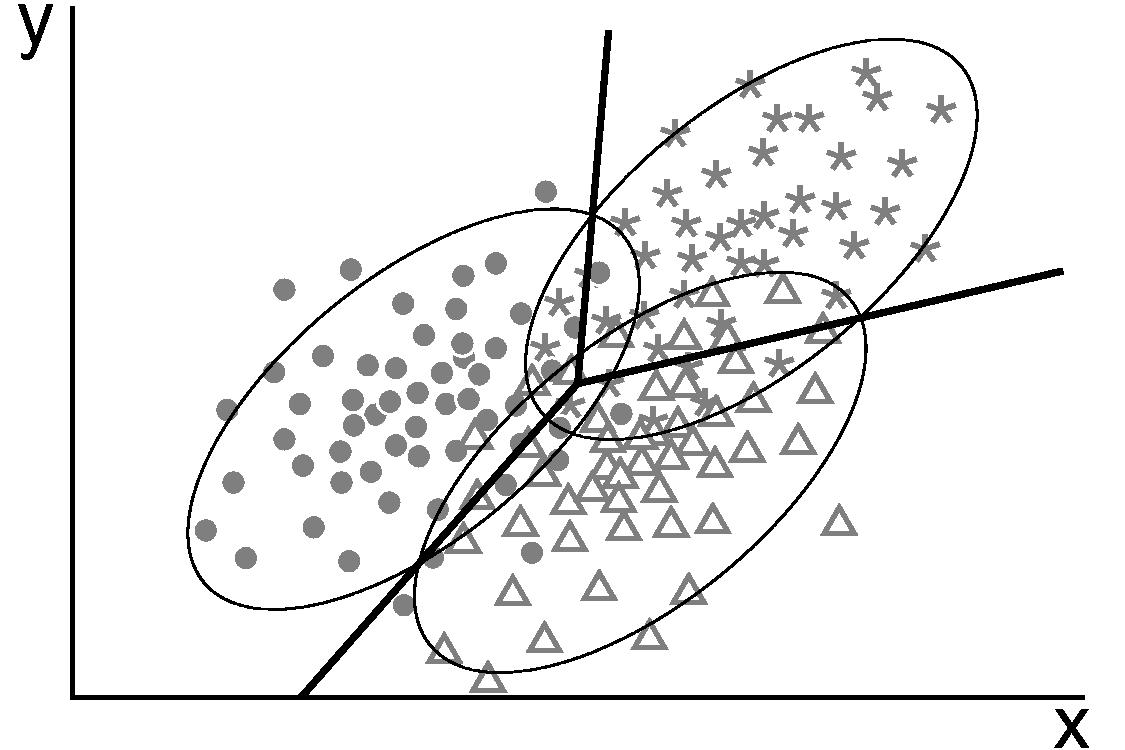
\includegraphics[width=400]{figures/discriminant.jpg}
  \caption[Linear discriminant analysis]{
Discriminant analysis of three  classes with equal covariance matrices
leads to  linear discriminant boundaries. The  ellipses mark arbitrary
(e.g., 95\%) confidence levels for the underlying populations.}
\end{figure}

\begin{figure}[htbp]
  \centering
  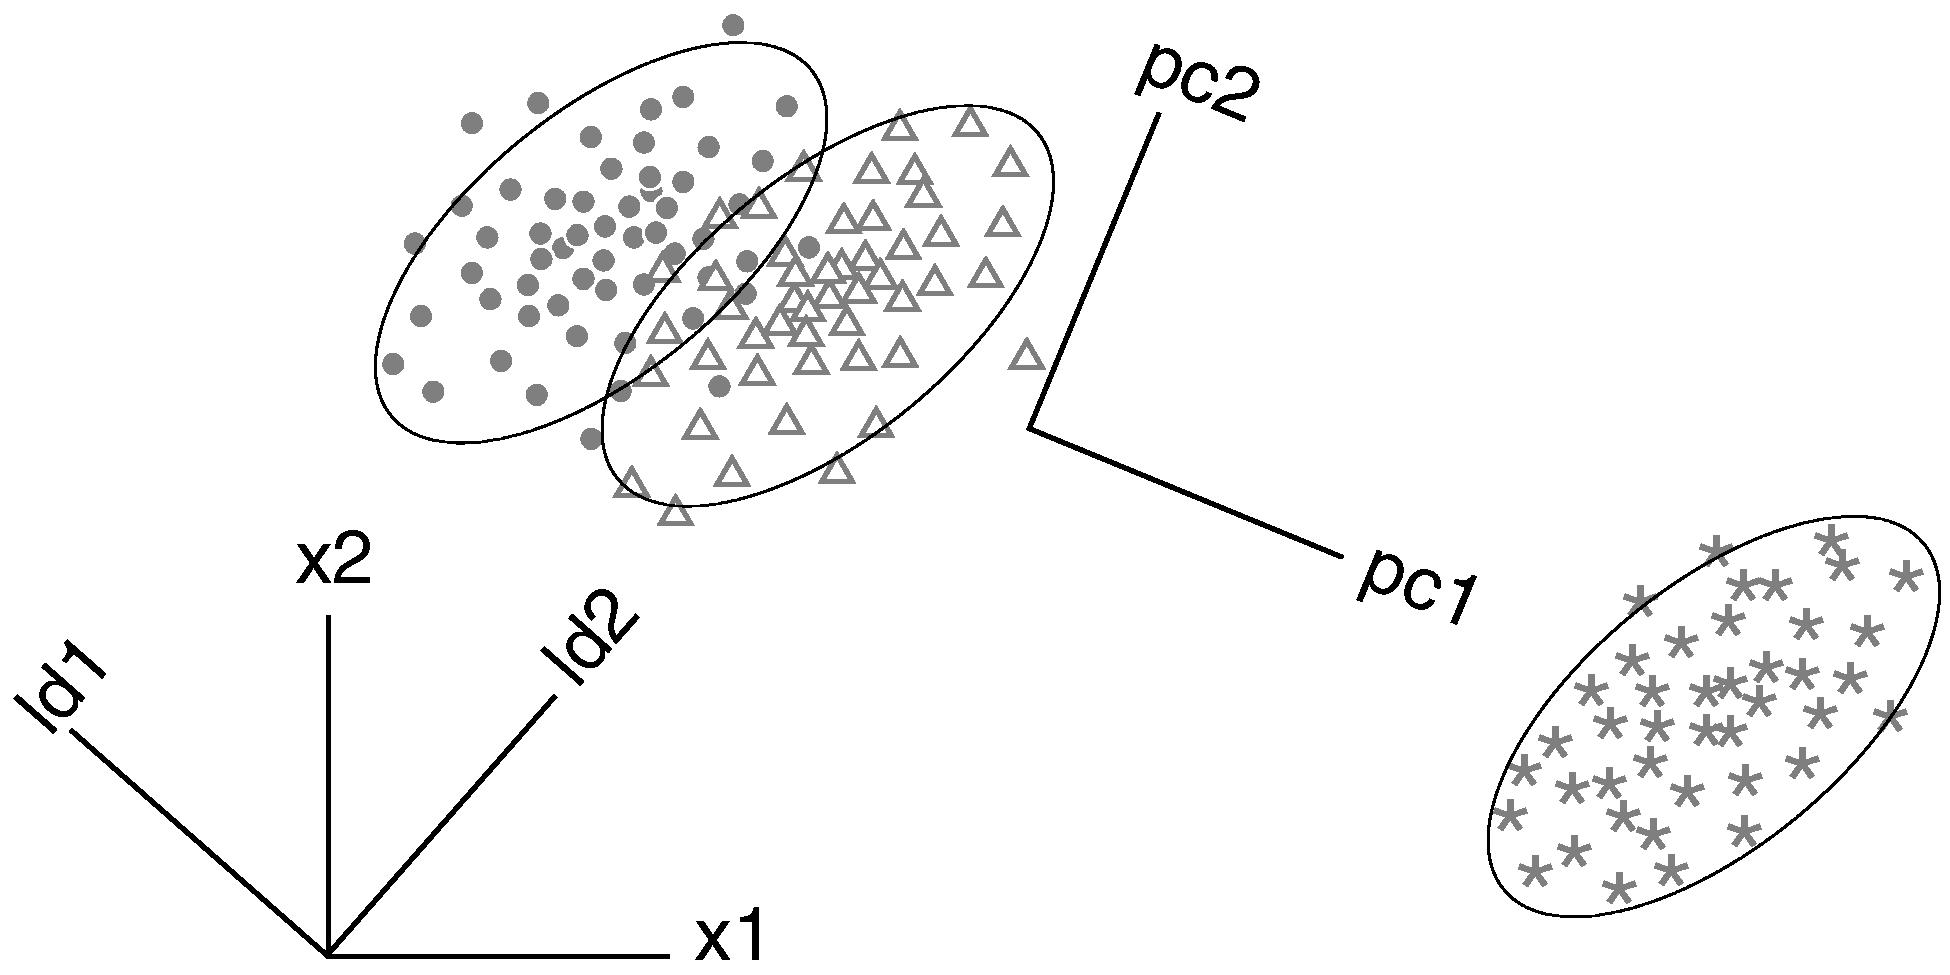
\includegraphics[width=600]{figures/PCAvsLDA.jpg}
  \caption[The difference between PCA and LDA]
{Similarities   and  differences   between  linear   discriminant  and
principal component  analysis.  x1 and x2 are  the original variables,
pc1  and pc2  are the  principal components  and ld1  and ld2  are the
linear discriminant functions.}
  \label{fig:PCAvsLDA}
\end{figure}

\begin{figure}[htbp]
  \centering
  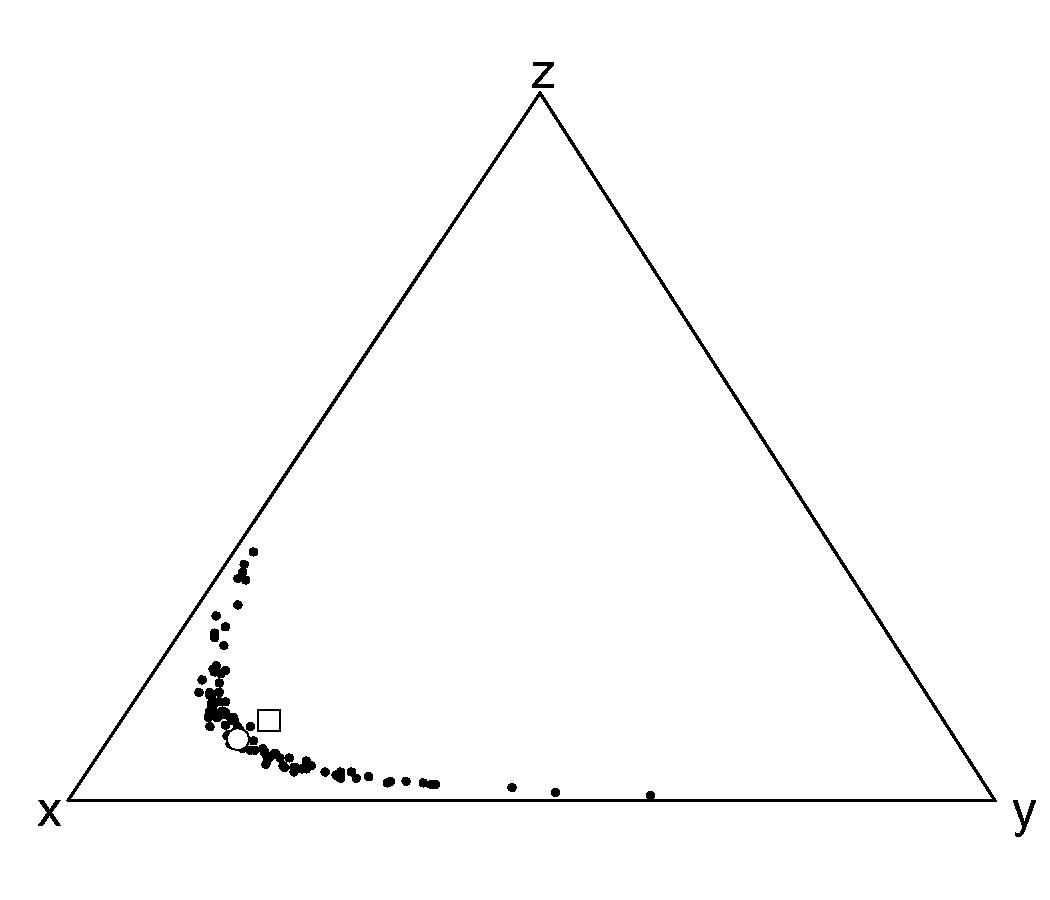
\includegraphics[width=400]{figures/closure.jpg}
  \caption[The consequences of the constant-sum constraint]
{One   of  the   consequences  of   the  constant-sum   constraint  of
compositional data  is that  the arithmetic mean  (marked by  the open
square) of populations (black  dots) has no physical meaning. Instead,
the geometric mean should be used (open circle).}
  \label{fig:closure}
\end{figure}

\begin{figure}[htbp]
  \centering
  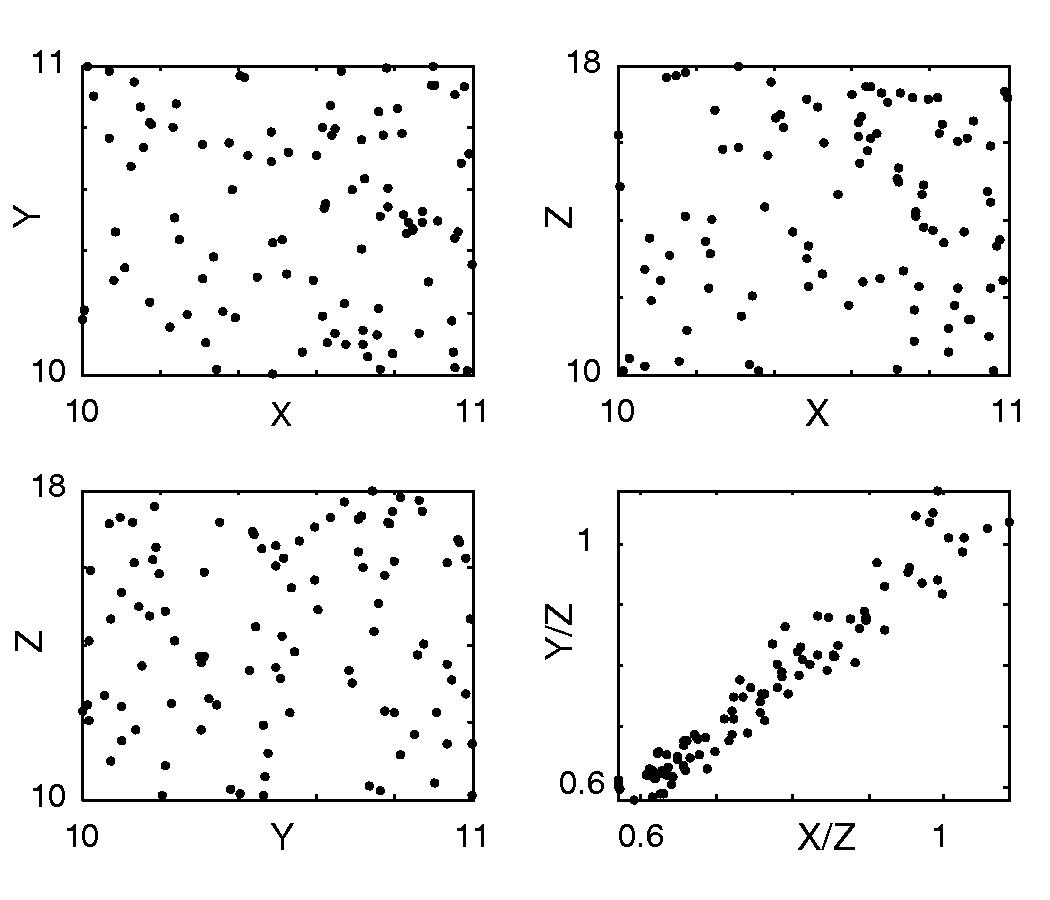
\includegraphics[width=600]{figures/spurious2.jpg}
  \caption[Spurious correlation of ratios]{X, Y and Z are uncorrelated, 
uniform random numbers. The  strong spurious correlation of the ratios
Y/Z  and X/Z  is an  artifact of  the relatively  large variance  of Z
relative to X, Y and Z.}
  \label{fig:spurious}
\end{figure}

\begin{figure}[htbp]
  \centering
  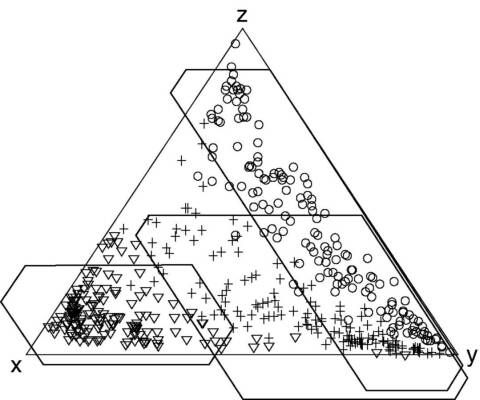
\includegraphics[width=400]{figures/closure_ternary_wrong2.jpg}
  \caption[The dangers of using ``traditional'' statistics on the simplex]{
95\%  normal confidence  regions  (e.g., Weltje,  2002) for  synthetic
trivariate compositional data partly fall outside the ternary diagram,
a   nonsense   result   illustrating   the   dangers   of   performing
``traditional'' statistics on the simplex.}
  \label{fig:closure_ternary_wrong}
\end{figure}

\begin{figure}[htbp]
  \centering
  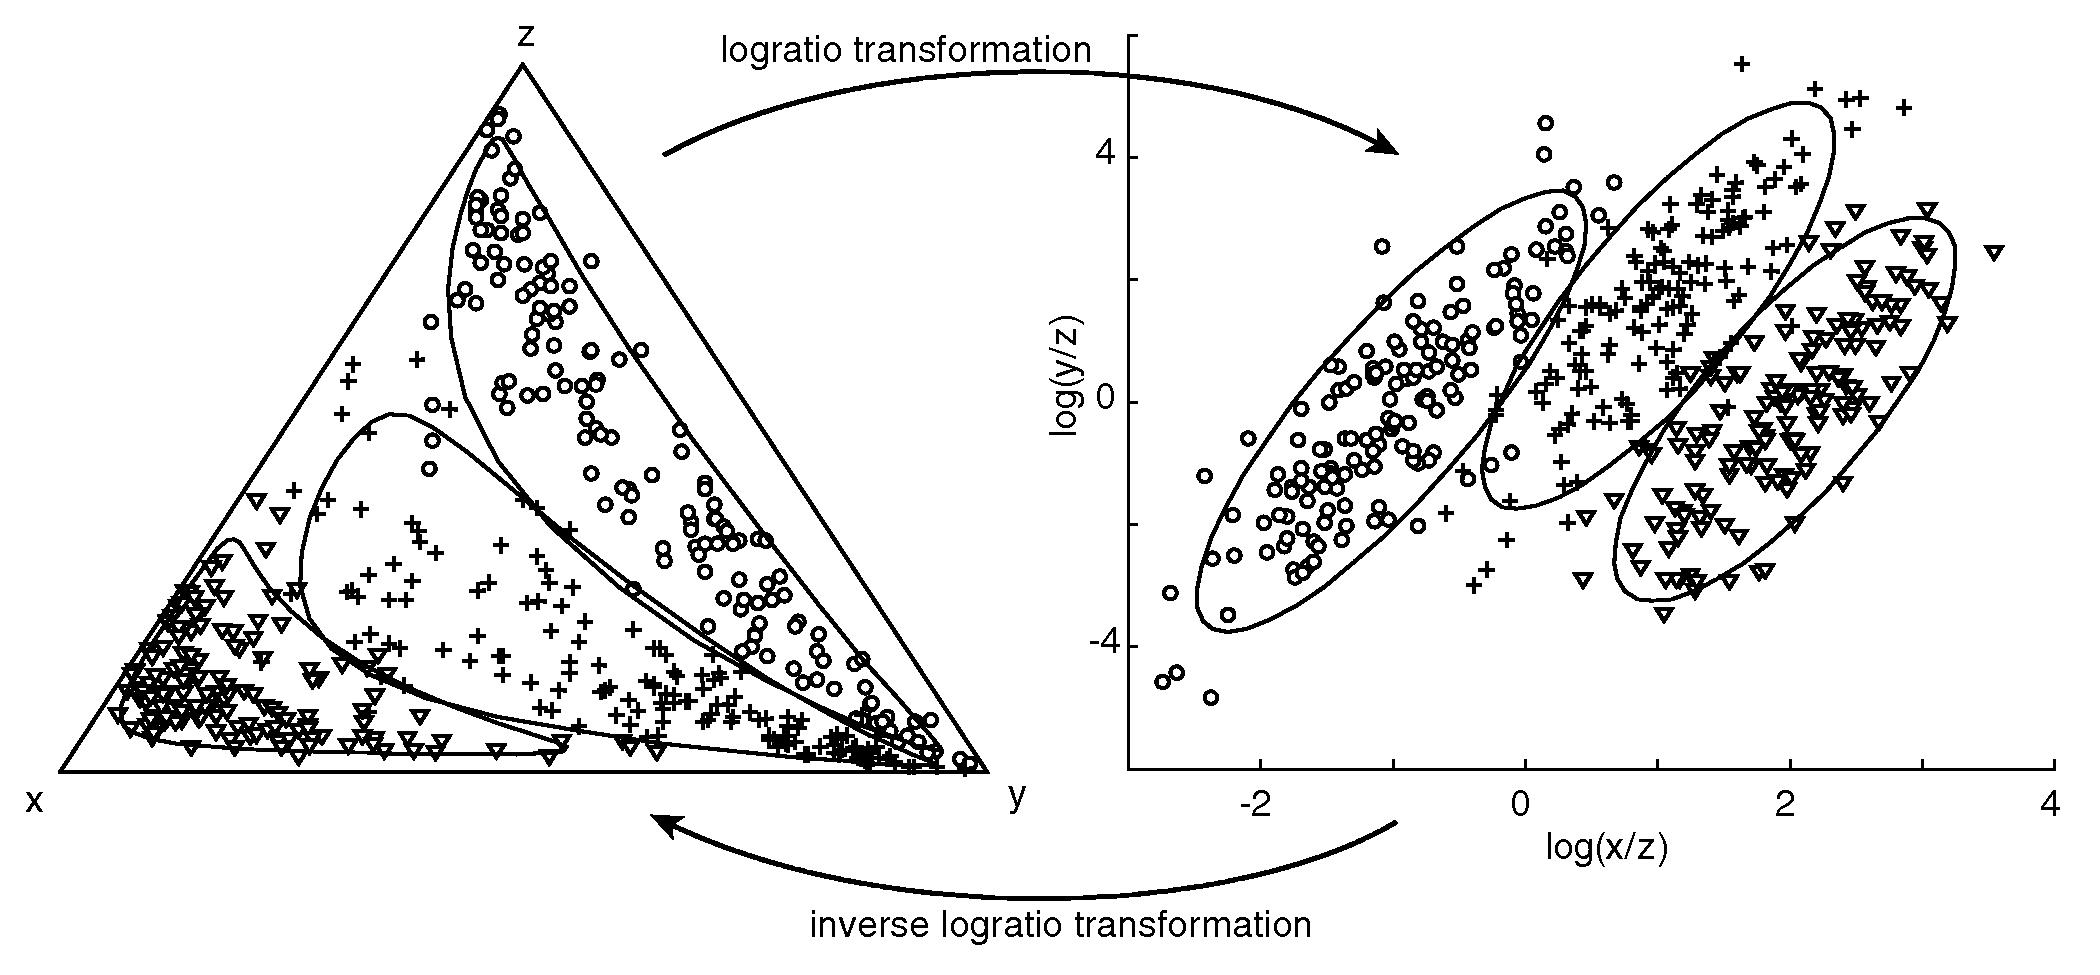
\includegraphics[width=600]{figures/closure_mapping.jpg}
  \caption[Mapping compositional data from $\Delta_2$  to  $\mathbb{R}^2$]{
Following  Aitchison  (1986),   the  statistical  problems  of  Figure
\ref{fig:closure_ternary_wrong}  can be  avoided by  mapping  the data
from  the  simplex $\Delta_2$  to  $\mathbb{R}^2$  using the  logratio
transformation.}
  \label{fig:closure_mapping}
\end{figure}

\begin{figure}[htbp]
  \centering
  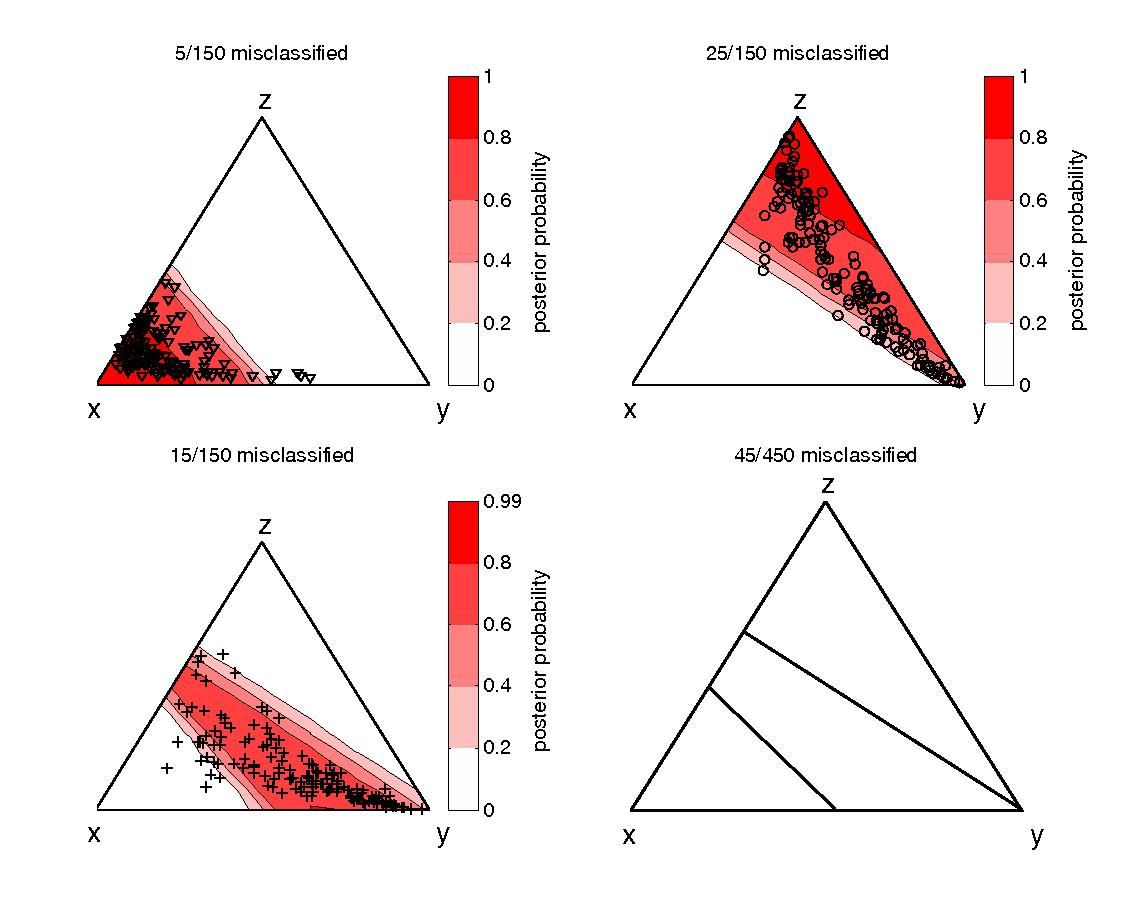
\includegraphics[width=600]{figures/closure_discriminant_wrong.jpg}
  \caption[Linear discriminant analysis done the wrong way]{
Linear discriminant analysis using the {\it crude covariance} approach
of Figure \ref{fig:closure_ternary_wrong}.  The red-shaded contours of
the first three ternary diagrams represent the posterior probabilities
for the  three classes.   The last diagram  shows the  linear decision
boundaries. 10\% of the training data are misclassified.}
  \label{fig:closure_discriminant_wrong}
\end{figure}

\begin{figure}[htbp]
  \centering
  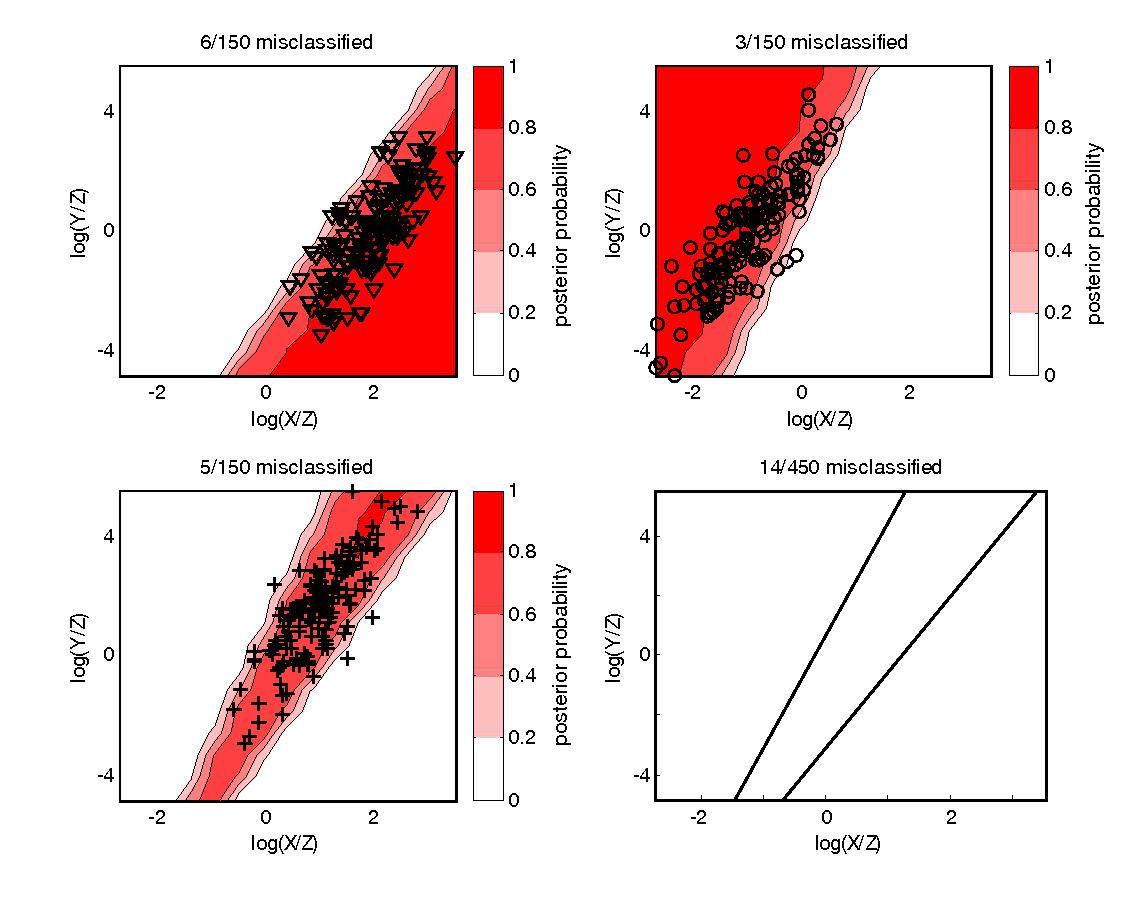
\includegraphics[width=600]{figures/closure_binary_discriminant_right.jpg}
\caption[Linear discriminant analysis done the right way]{
The same  data of Figure  \ref{fig:closure_discriminant_wrong}, mapped
to   logratio-space   using  the   approach   illustrated  by   Figure
\ref{fig:closure_mapping}.  Linear   discriminant  analysis  of  these
bivariate data misclassifies only 3\% of the training data.}
  \label{fig:closure_binary_discriminant_right}
\end{figure}

\begin{figure}[htbp]
  \centering
  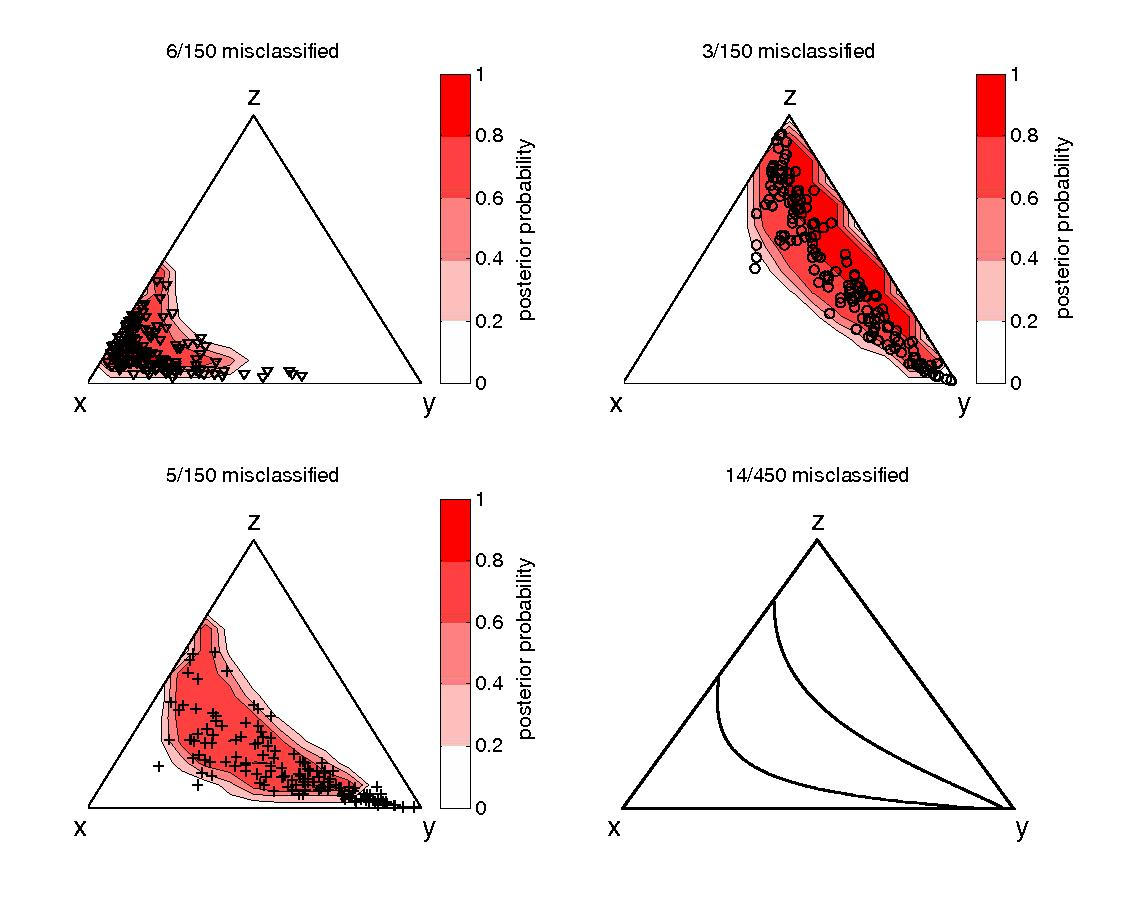
\includegraphics[width=600]{figures/closure_ternary_discriminant_right.jpg}
  \caption[Results of the linear discriminant analysis mapped back to the simplex]{
Mapping the  results of Figure \ref{fig:closure_binary_discriminant_right} 
back  to the ternary  diagram with  the  inverse logratio  transformation shown  on
Figure \ref{fig:closure_mapping} yields curved posterior densities and
decision boundaries.}
  \label{fig:closure_ternary_discriminant_right}
\end{figure}

\begin{figure}[htbp]
  \centering
  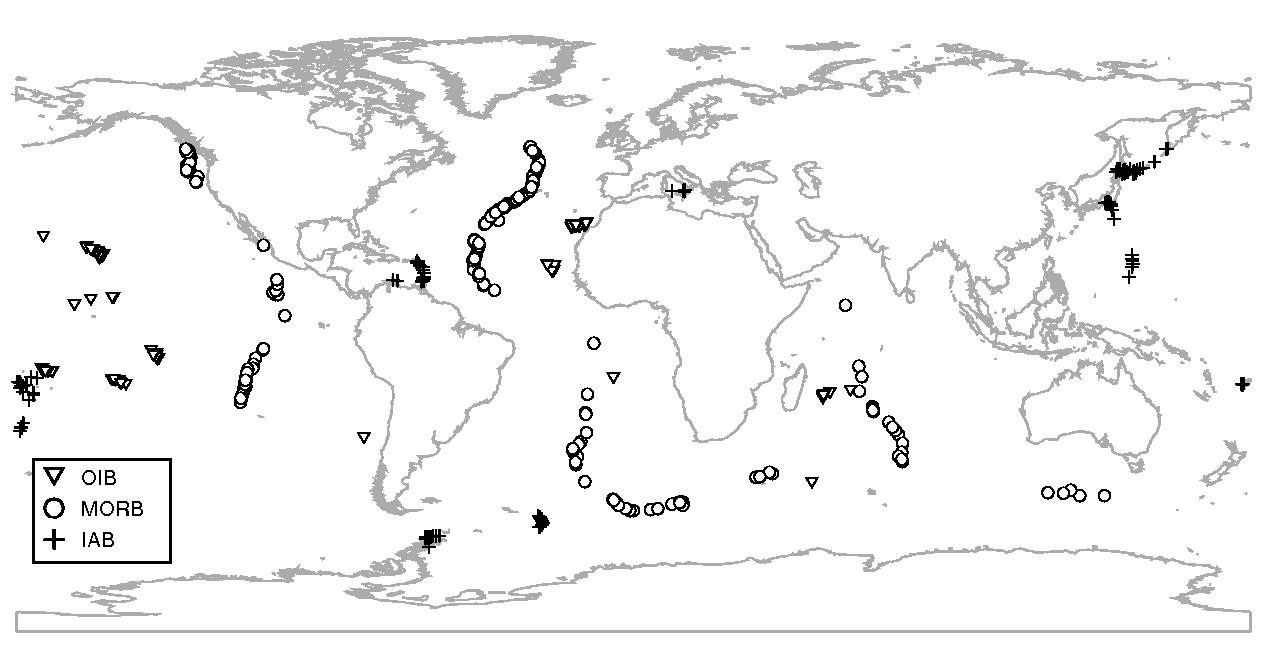
\includegraphics[width=600]{figures/sample_locations.jpg}
  \caption[Geographical locations of the training data]{
Locations of the training data:  756 Island Arc (IAB), Mid Ocean Ridge
(MORB) and Ocean Island (OIB) Basalts.}
  \label{fig:sample_locations}
\end{figure}

\clearpage

\begin{figure}[htbp]
  \centering
  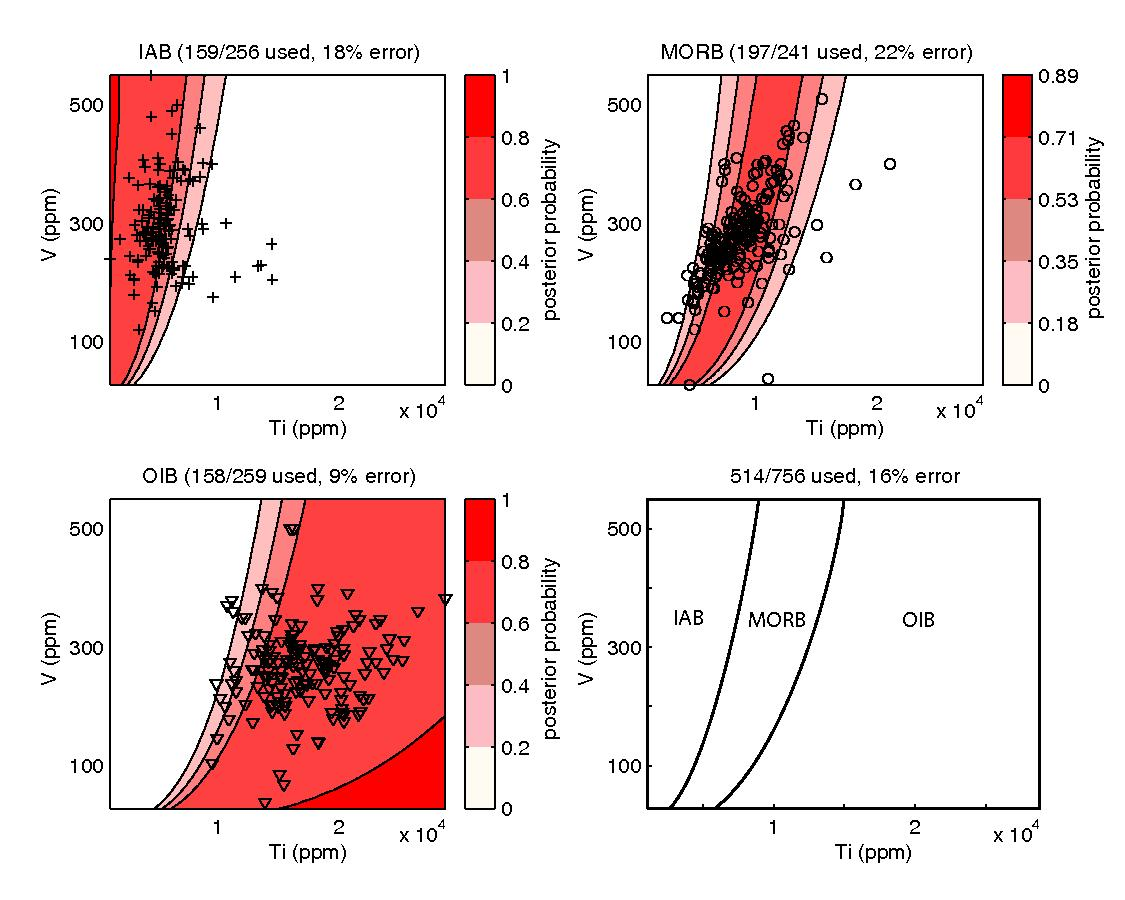
\includegraphics[width=600]{figures/Ti_V_lin.jpg}
  \caption[Linear discriminant analysis of the Ti-V system of Shervais (1982)]
{Linear  discriminant analysis (LDA)  of the  Ti-V system  of Shervais
(1982).  The red-shaded contours on  the first three subplots show the
posterior probability  of a particular  ``class'' (IAB, MORB,  or OIB)
given the training set of 756  basalt samples and a uniform prior. The
last  subplot (lower-right)  shows the  new decision  boundaries.  The
number of training  data used and a resubstitution  error estimate are
given for each of the tectonic affinities.  The overall resubstitution
error is shown above the lower-right subplot.}
  \label{fig:Ti_V_lin}
\end{figure}

\begin{figure}[htbp]
  \centering
  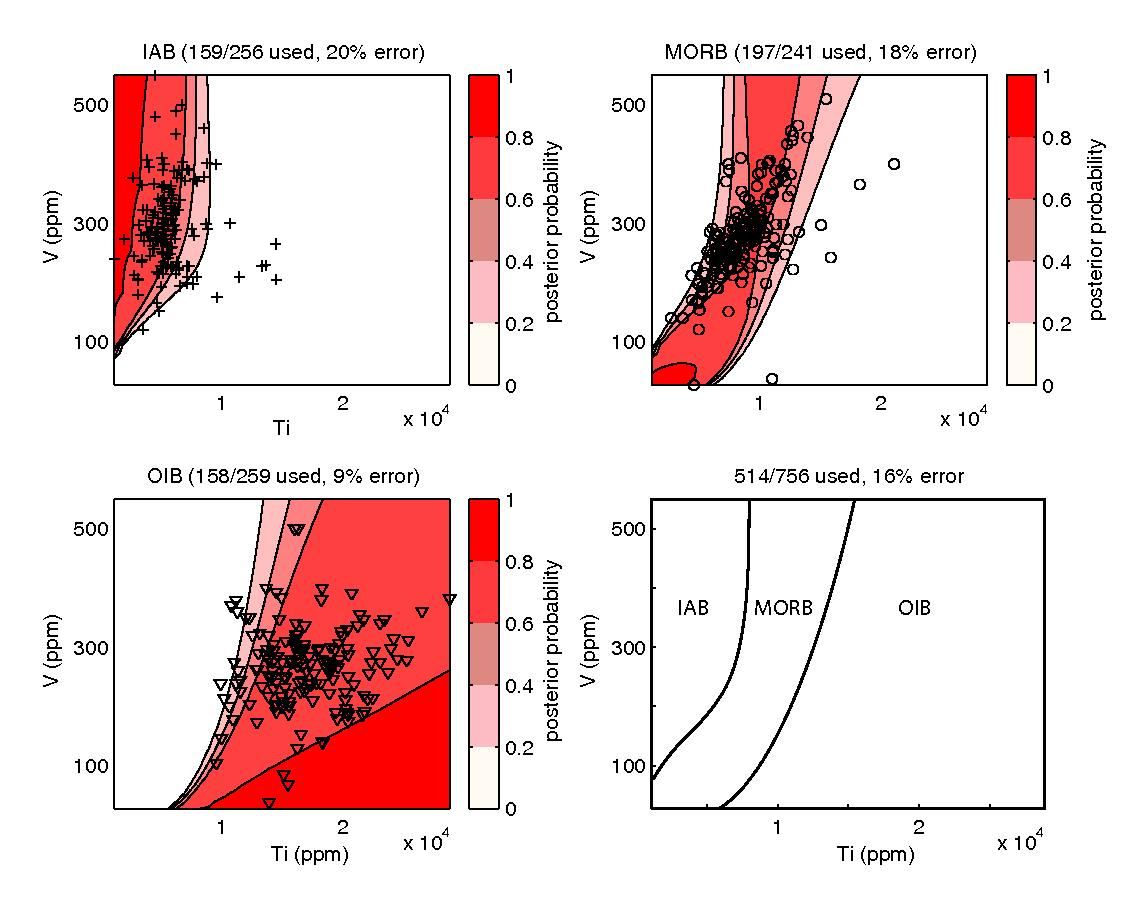
\includegraphics[width=600]{figures/Ti_V_quad.jpg}
  \caption[Quadratic discriminant analysis of the Ti-V system]
{Quadratic discriminant analysis (QDA) of the Ti-V system. In contrast
with the LDA of Figure \ref{fig:Ti_V_lin}, each tectonic ``class'' was
allowed to  have a different covariance matrix,  resulting in slightly
different decision boundaries.}
  \label{fig:Ti_V_quad}
\end{figure}

\begin{figure}[htbp]
  \centering
  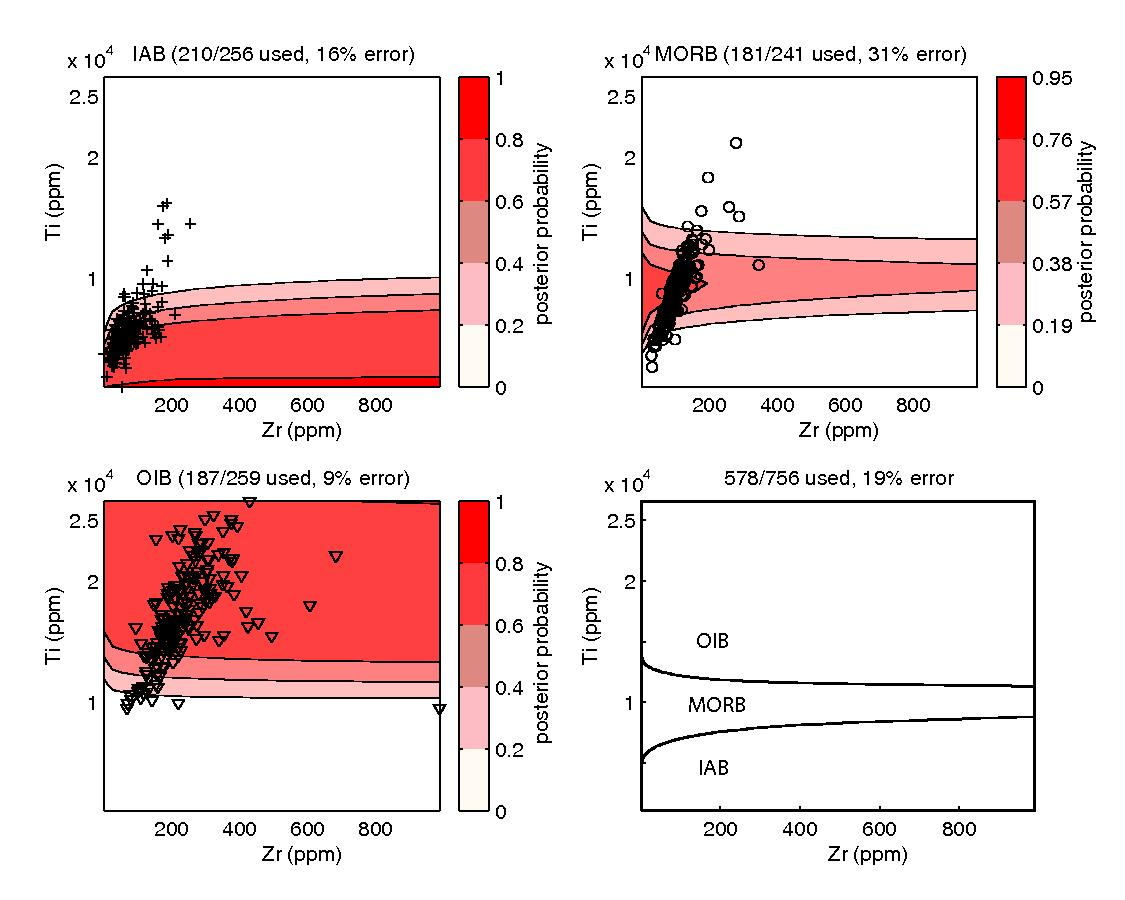
\includegraphics[width=600]{figures/Ti_Zr_lin.jpg}
  \caption[Linear discriminant analysis of the Ti-Zr system of Pearce and Cann (1973)]
{Linear discriminant analysis of the Ti-Zr system of Pearce and Cann (1973).}
  \label{fig:Ti_Zr_lin}
\end{figure}

\begin{figure}[htbp]
  \centering
  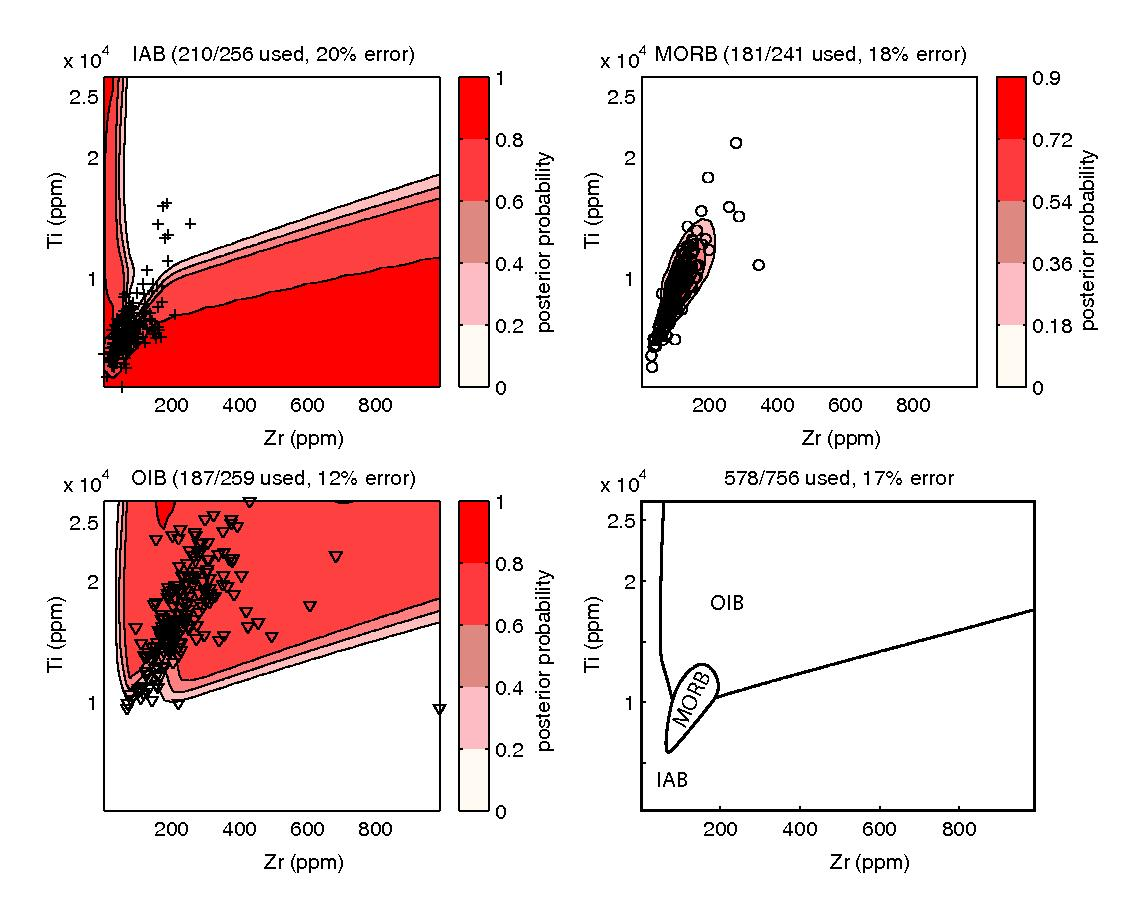
\includegraphics[width=600]{figures/Ti_Zr_quad.jpg}
  \caption[Quadratic discriminant analysis of the Ti-Zr system]
{Quadratic discriminant analysis of the Ti-Zr system.}
  \label{fig:Ti_Zr_quad}
\end{figure}

\begin{figure}[htbp]
  \centering
  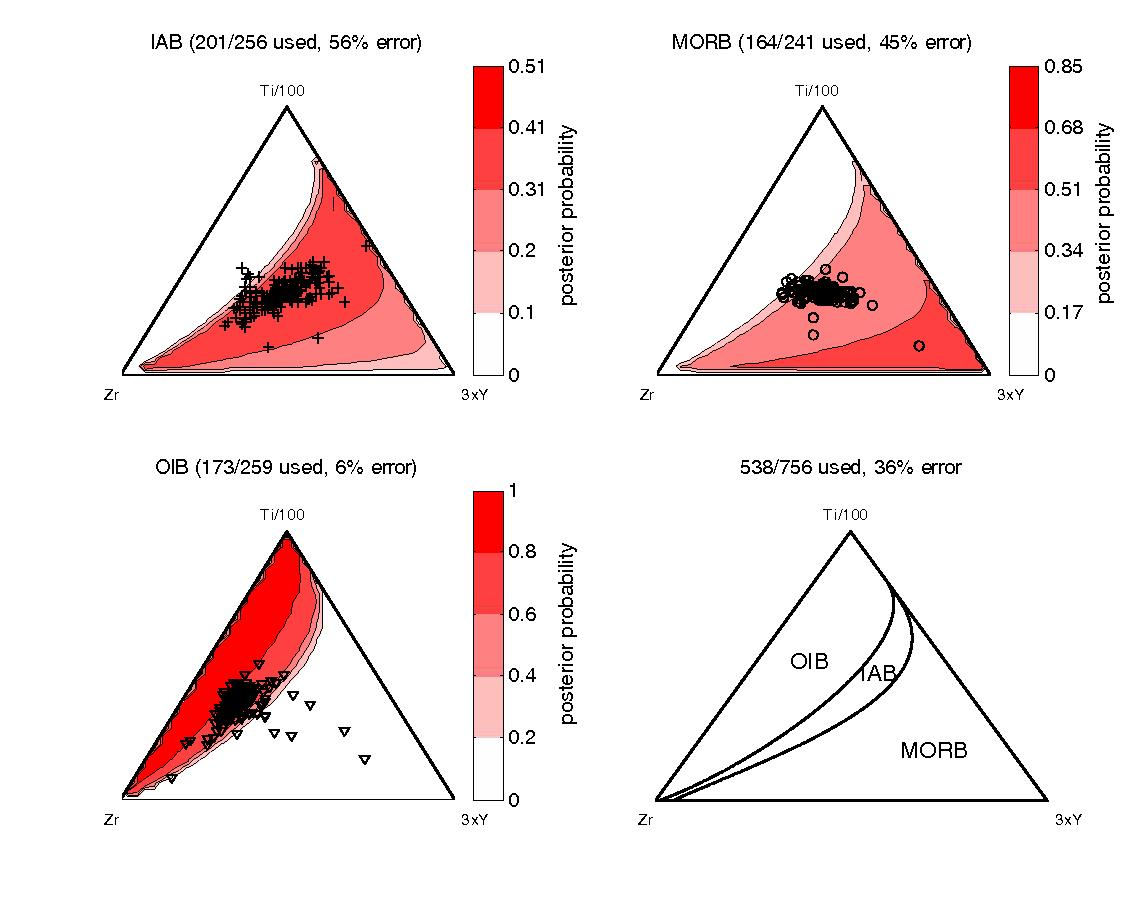
\includegraphics[width=600]{figures/Ti_Zr_Y_lin.jpg}
  \caption[Linear discriminant analysis of the Ti-Zr-Y system of Pearce and Cann (1973)]
{Linear discriminant analysis of the Ti-Zr-Y system of Pearce and Cann
(1973).  The  posterior probabilities of  nearly all the IAB  and MORB
training data  are low ($<$0.4), resulting  in large misclassification
rates for  these affinities. As noted  by Pearce and  Cann (1973), the
Ti-Zr-Y  diagram can  be used  to  separate OIBs  from IAB/MORBs,  but
cannot be used to distinguish  between IAB and MORB. For this purpose,
the Ti-Zr diagram (Figure \ref{fig:Ti_Zr_lin}) can be used.}
  \label{fig:Ti_Zr_Y_lin}
\end{figure}

\begin{figure}[htbp]
  \centering
  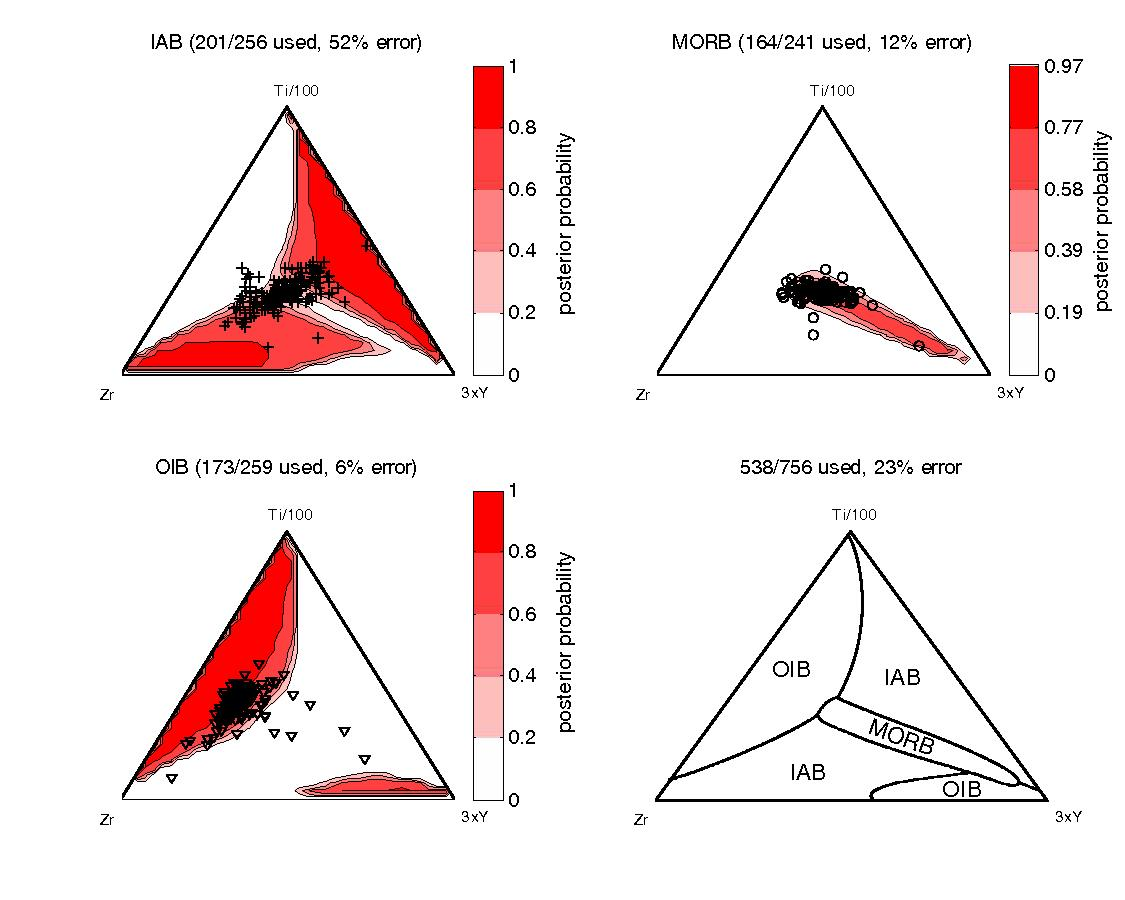
\includegraphics[width=600]{figures/Ti_Zr_Y_quad.jpg}
  \caption[Quadratic discriminant analysis of the Ti-Zr-Y system]
{Quadratic discriminant  analysis of the Ti-Zr-Y  system.  The OIB/IAB
decision boundary  (at low  Y) is nearly  identical to that  of Figure
\ref{fig:Ti_Zr_Y_lin},  whereas   there  is  a   lot  more  (unstable)
structure at higher Y concentrations.}
  \label{fig:Ti_Zr_Y_quad}
\end{figure}

\begin{figure}[htbp]
  \centering
  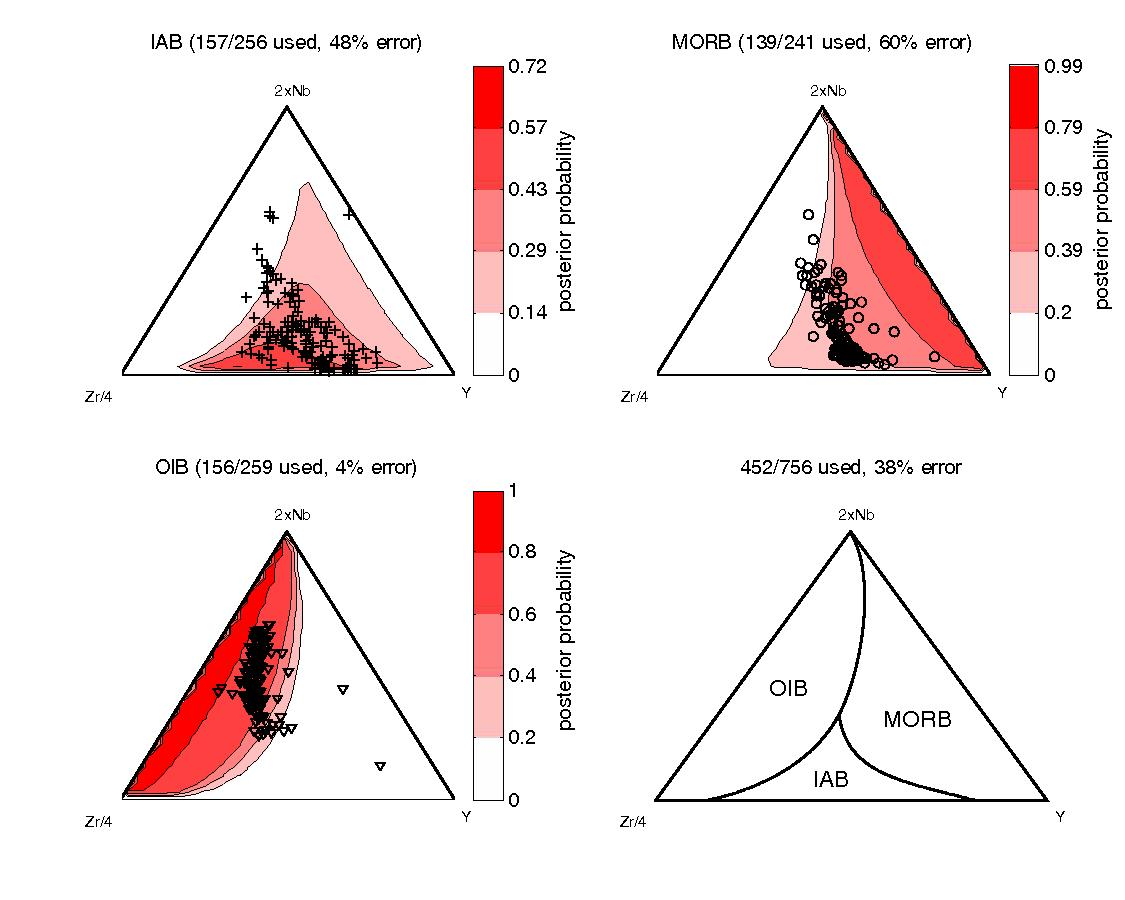
\includegraphics[width=600]{figures/Nb_Zr_Y_lin.jpg}
  \caption[Linear discriminant analysis of the Zr-Y-Nb system of Meschede (1986)]
{Linear  discriminant  analysis  of  the Zr-Y-Nb  system  of  Meschede
(1986). Like  in Figure \ref{fig:Ti_Zr_Y_lin}, posterior  IAB and MORB
probabilities are low, resulting in high misclassification rates.}
  \label{fig:Nb_Zr_Y_lin}
\end{figure}

\begin{figure}[htbp]
  \centering
  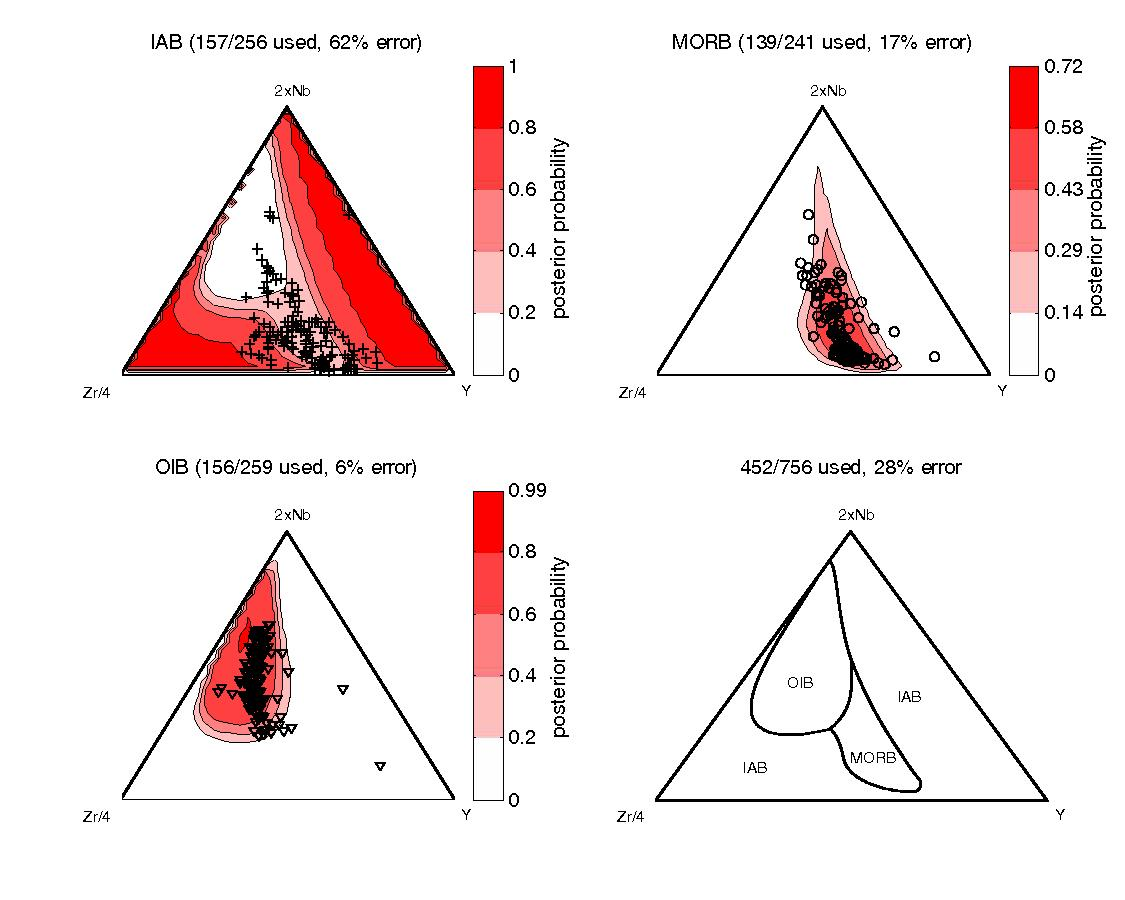
\includegraphics[width=600]{figures/Nb_Zr_Y_quad.jpg}
  \caption[Quadratic discriminant analysis of the Zr-Y-Nb system]
{Quadratic discriminant analysis of the Zr-Y-Nb system.}
  \label{fig:Nb_Zr_Y_quad}
\end{figure}

\begin{figure}[htbp]
  \centering
  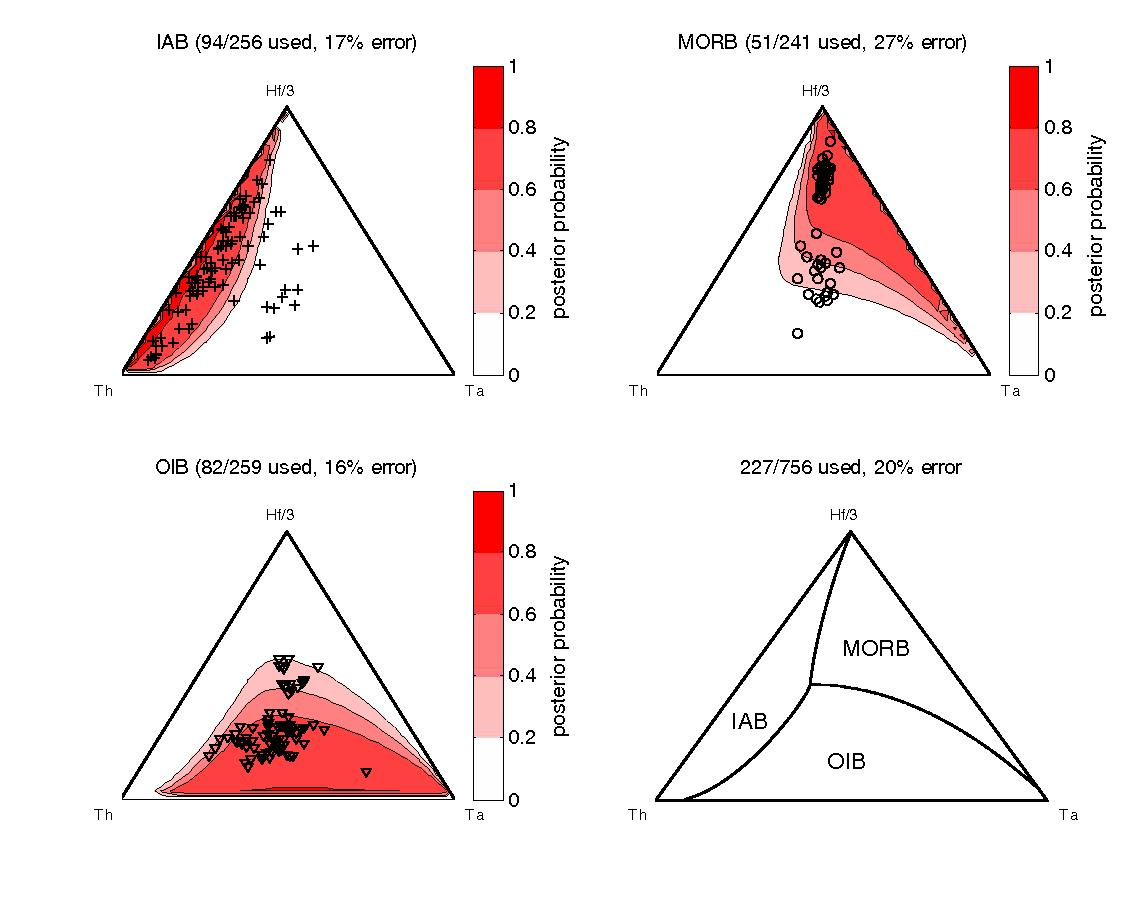
\includegraphics[width=600]{figures/Th_Ta_Hf_lin.jpg}
  \caption[Linear discriminant analysis of the Th-Ta-Hf system of Wood (1980)]
{Linear discriminant analysis of the Th-Ta-Hf system of Wood (1980).}
  \label{fig:Th_Ta_Hf_lin}
\end{figure}

\begin{figure}[htbp]
  \centering
  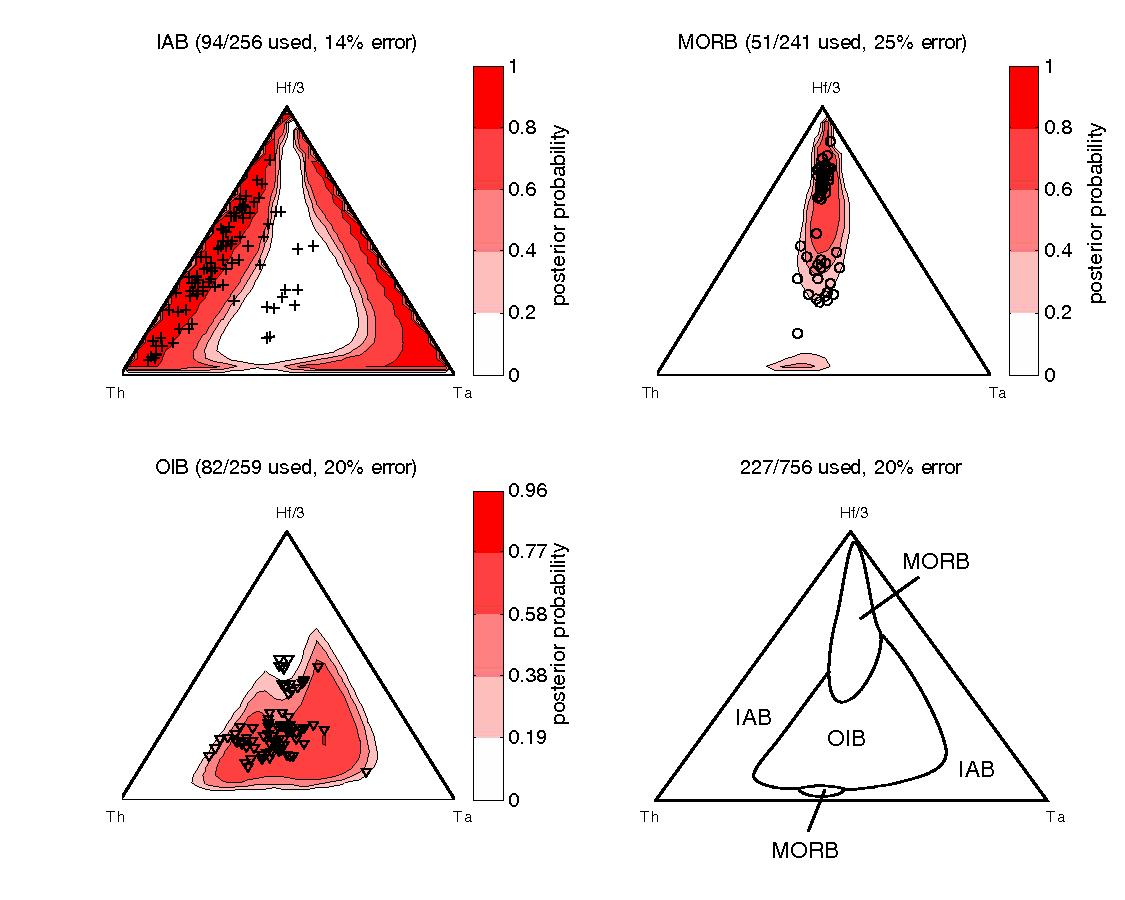
\includegraphics[width=600]{figures/Th_Ta_Hf_quad.jpg}
  \caption[Quadratic discriminant analysis of the Th-Ta-Hf system]
{Quadratic discriminant analysis of the Th-Ta-Hf system.}
  \label{fig:Th_Ta_Hf_quad}
\end{figure}

\clearpage

\begin{figure}[htbp]
  \centering
  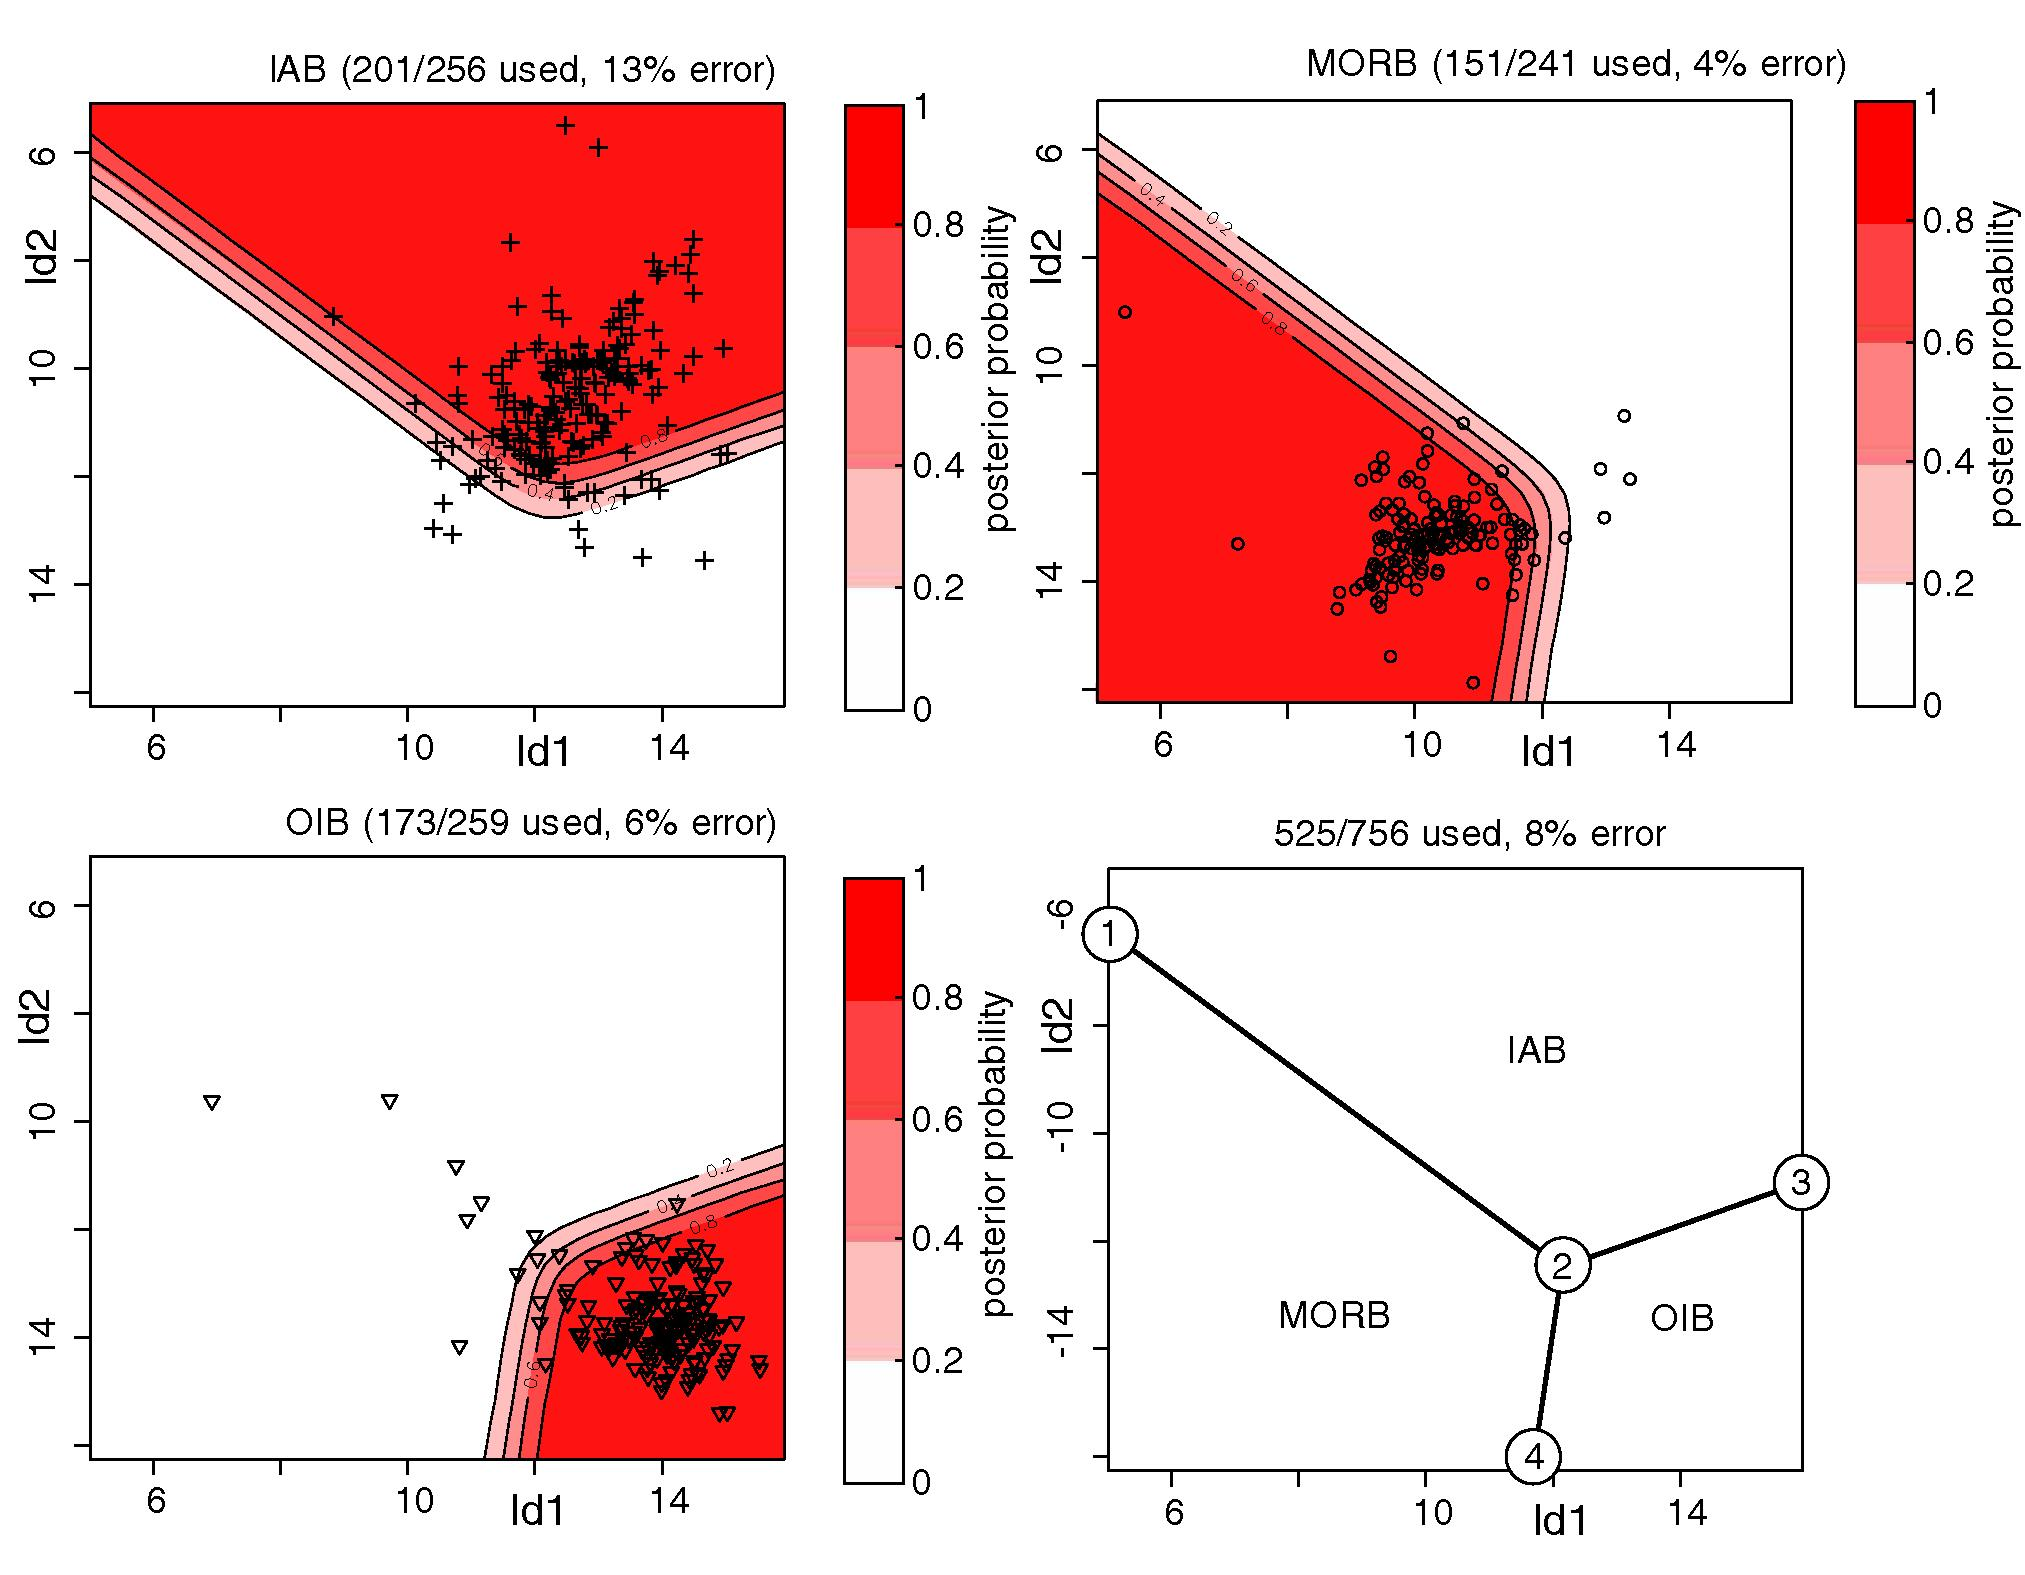
\includegraphics[width=600]{figures/discrimiFunc2.jpg}
  \caption[Linear discriminant analysis using Ti, Zr, Y and Sr]{
Linear discriminant analysis of the Ti-Zr-Y-Sr system. ld1 and ld2 are
the   two   linear   discriminant   functions,   given   by   Equation
\ref{eq:ld_a}.   They represent two  projection planes  that optimally
separate the three tectonic affinities  (IAB, MORB, and OIB) (see also
Figure \ref{fig:PCAvsLDA}).  The encircled  numbers on the lower right
subplot  are  ``anchor  points'' that  can  be  used  by the  user  to
reconstruct  the decision boundaries  in logratio-space.   The ld1/ld2
coordinates   of   these   anchor    points   are   given   in   Table
\ref{tab:anchors}.}
  \label{fig:discrimiFunc1}
\end{figure}

\begin{figure}[htbp]
  \centering
  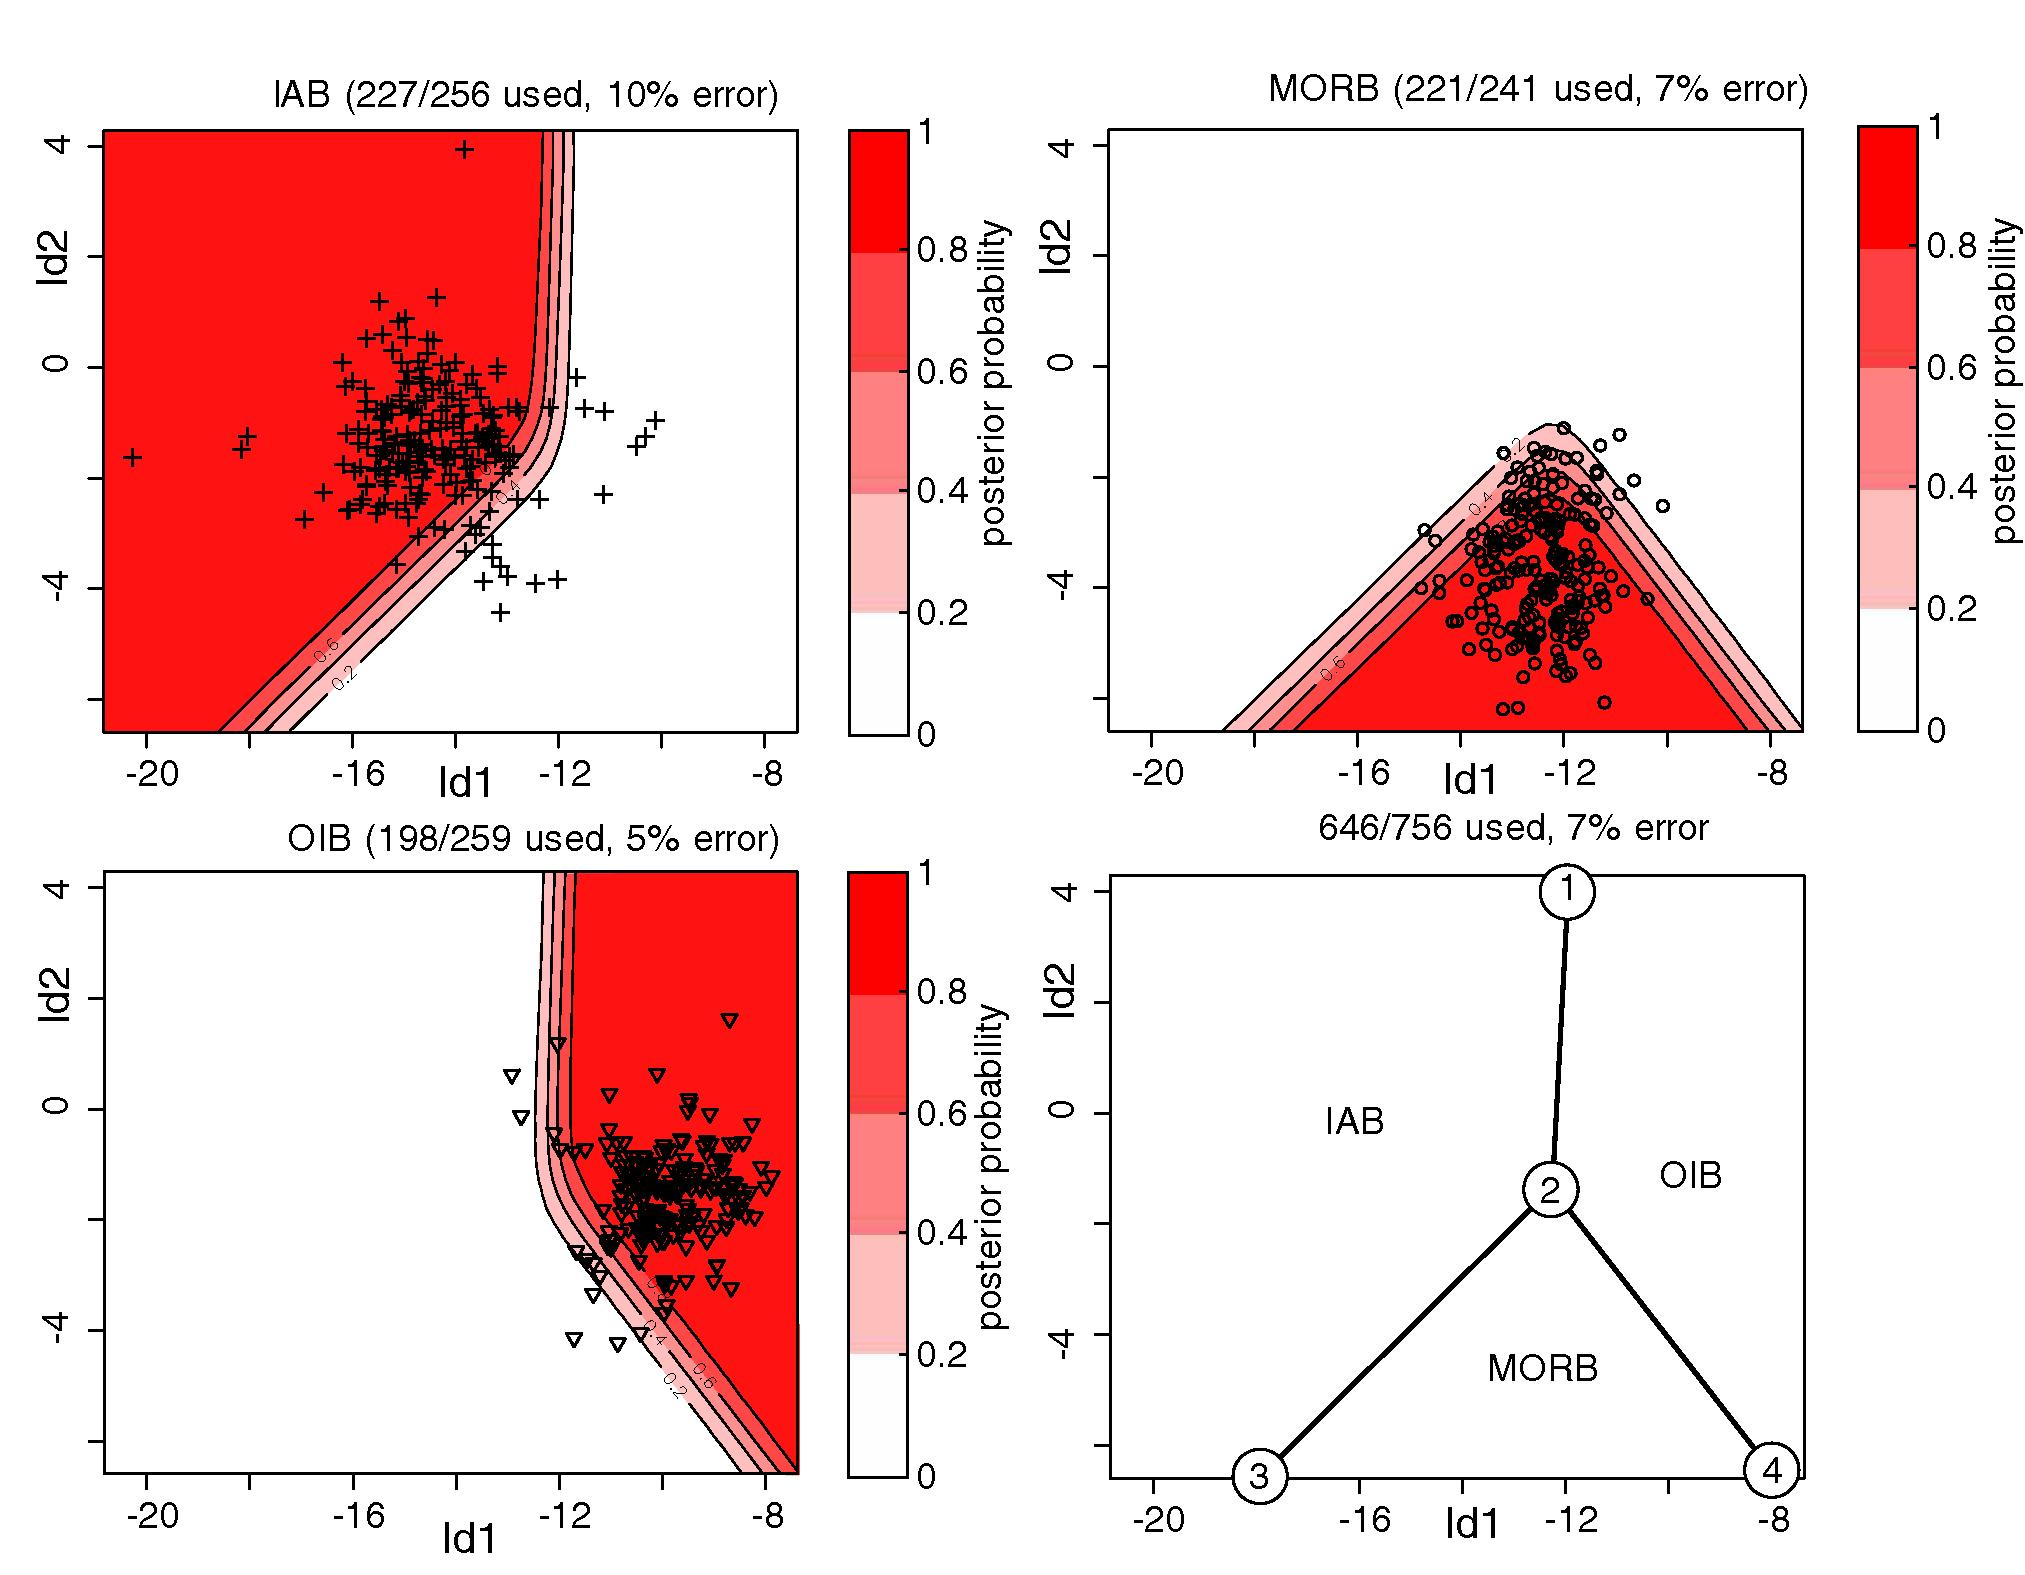
\includegraphics[width=600]{figures/discrimiFunc1.jpg}
  \caption[Linear discriminant analysis using major element data]{
Linear   discriminant  analysis  of   major  element   data  (SiO$_2$,
Al$_2$O$_3$,  TiO$_2$,  CaO, MgO,  MnO,  K$_2$O,  Na$_2$O), mapped  to
$\mathbb{R}^2$  using the  logratio  transformation. ld1  and ld2  are
given  by Equation  \ref{eq:ld_b}. Anchor  points are  given  in Table
\ref{tab:anchors}.}
  \label{fig:discrimiFunc2}
\end{figure}

\clearpage


\begin{figure}[htbp]
  \centering
  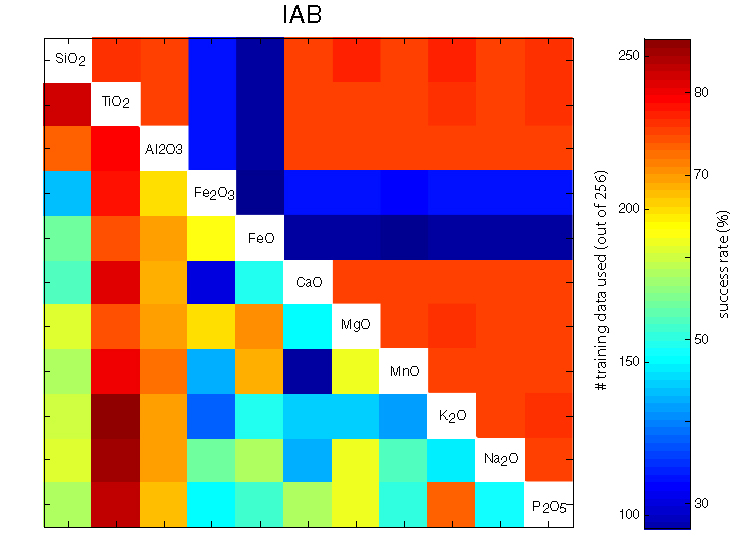
\includegraphics[width=300]{figures/xPlotMajor2_linear_IAB.jpg}
  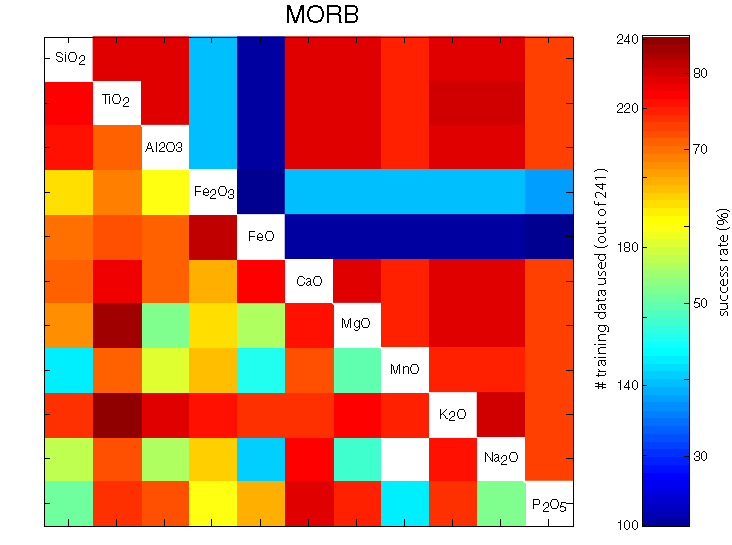
\includegraphics[width=300]{figures/xPlotMajor2_linear_MORB.jpg}\\
  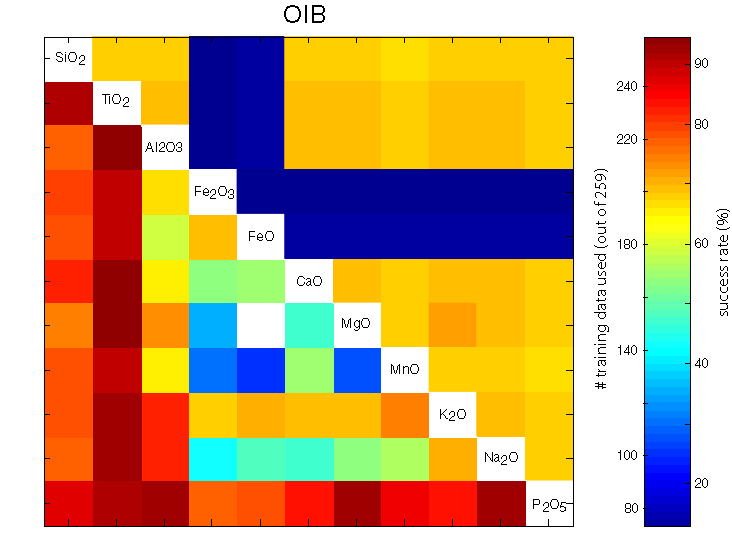
\includegraphics[width=300]{figures/xPlotMajor2_linear_OIB.jpg}
  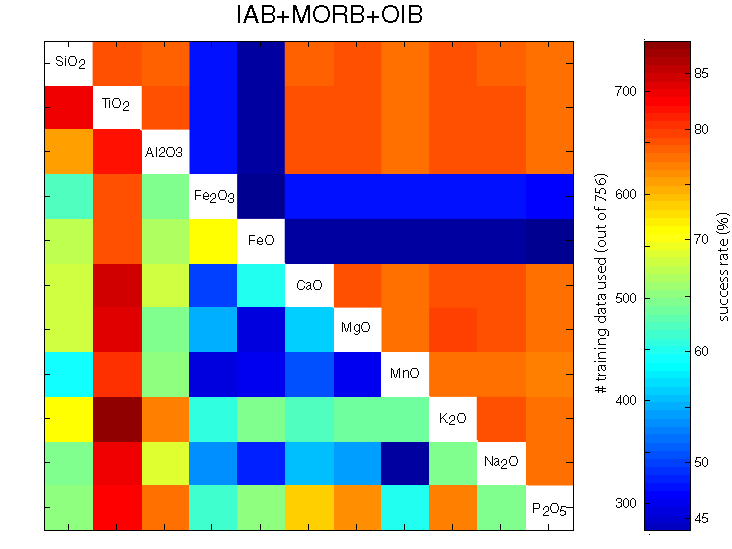
\includegraphics[width=300]{figures/xPlotMajor2_linear_err.jpg}
\caption[Exhaustive exploration of all bivariate linear discriminant 
analyses using only major elements]{
Visual  representation of  the performance  of all  possible bivariate
linear  discriminant analyses  using  the major  element  data of  the
training  set of  756  oceanic basalts.   The  upper right  triangular
section of each matrix shows the number of samples that contained both
variables.   The  lower  left  sections  color-code  the  fraction  of
successfully classified training data.}
  \label{fig:major2lin}
\end{figure}

\begin{figure}[htbp]
  \centering
  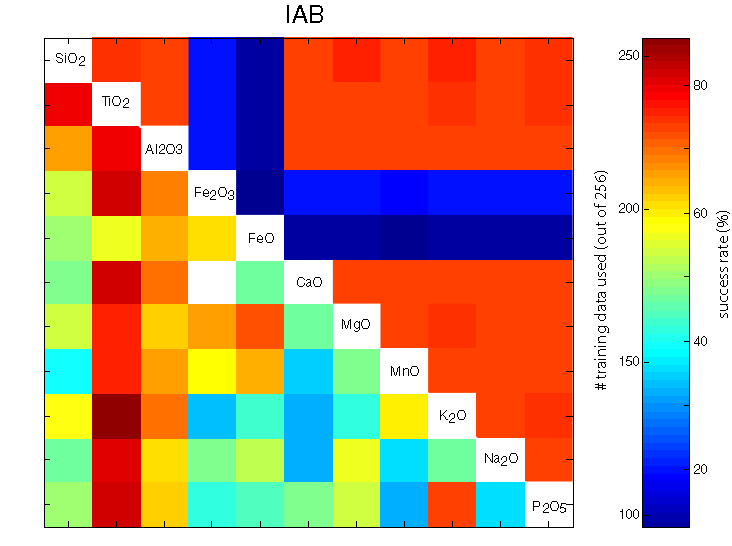
\includegraphics[width=300]{figures/xPlotMajor2_quadratic_IAB.jpg}
  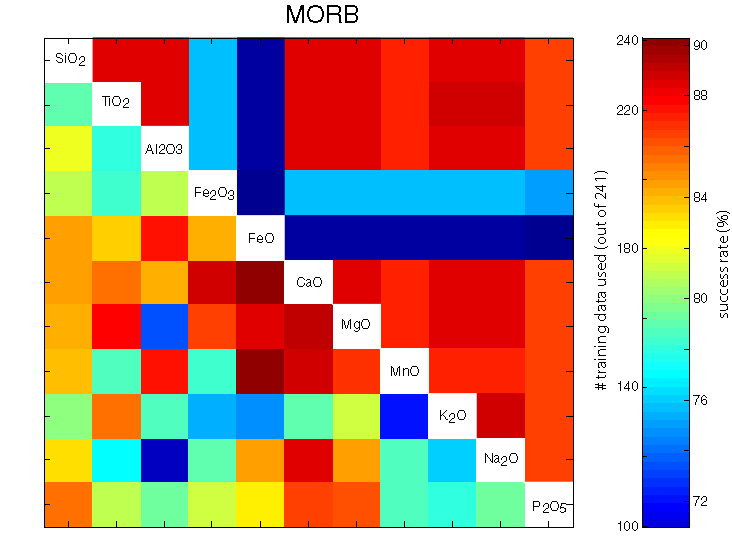
\includegraphics[width=300]{figures/xPlotMajor2_quadratic_MORB.jpg}\\
  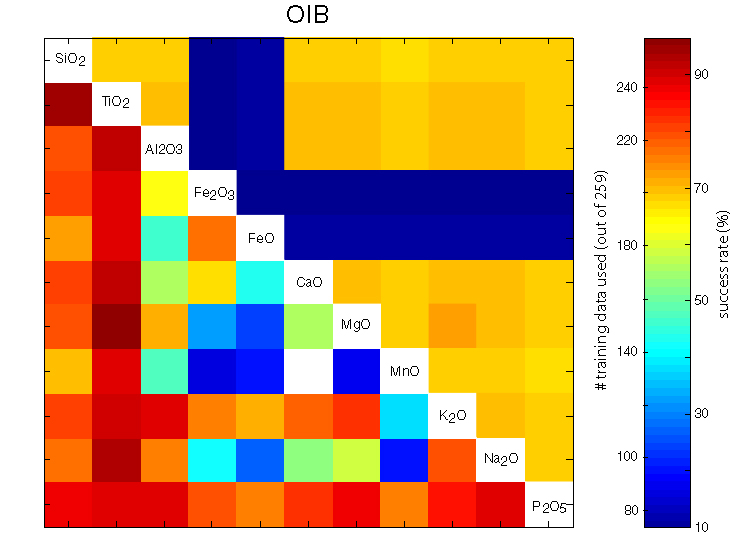
\includegraphics[width=300]{figures/xPlotMajor2_quadratic_OIB.jpg}
  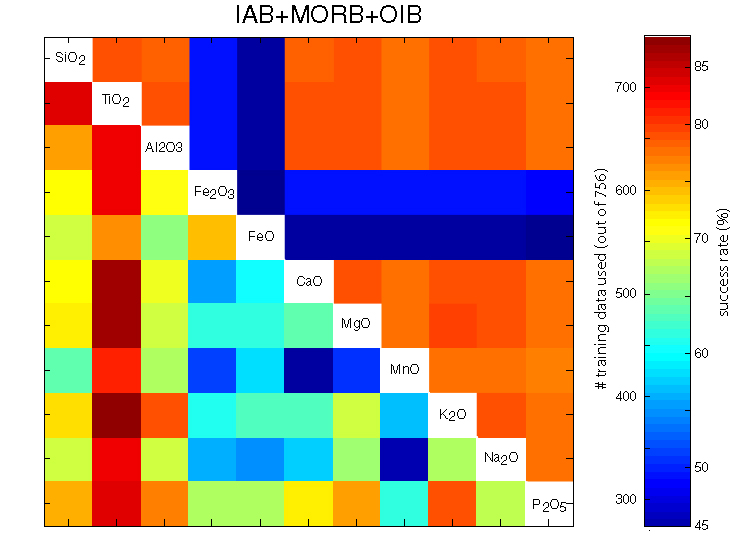
\includegraphics[width=300]{figures/xPlotMajor2_quadratic_err.jpg}
  \caption[Same  as Figure  \ref{fig:major2lin}, but  for
quadratic discriminant analysis]  {Same as Figure \ref{fig:major2lin},
but for quadratic discriminant analysis.}
  \label{fig:major2quad}
\end{figure}

\begin{figure}[htbp]
  \centering
  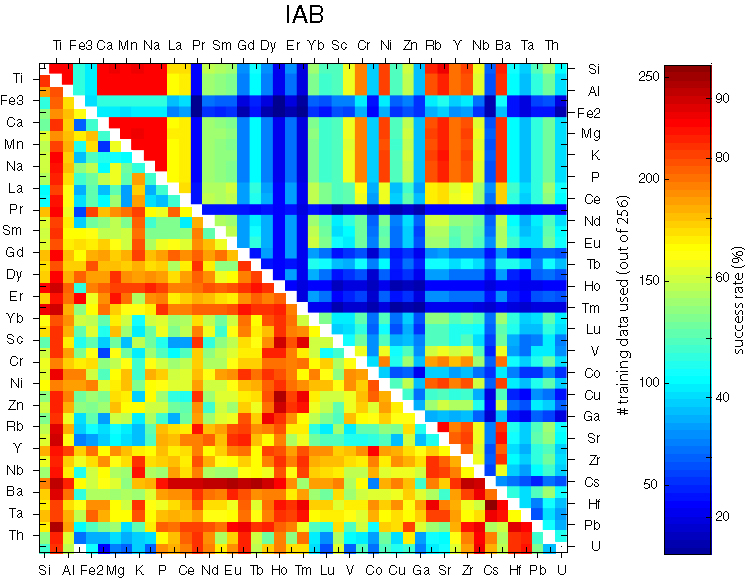
\includegraphics[width=300]{figures/xPlotTrace2_linear_IAB.jpg}
  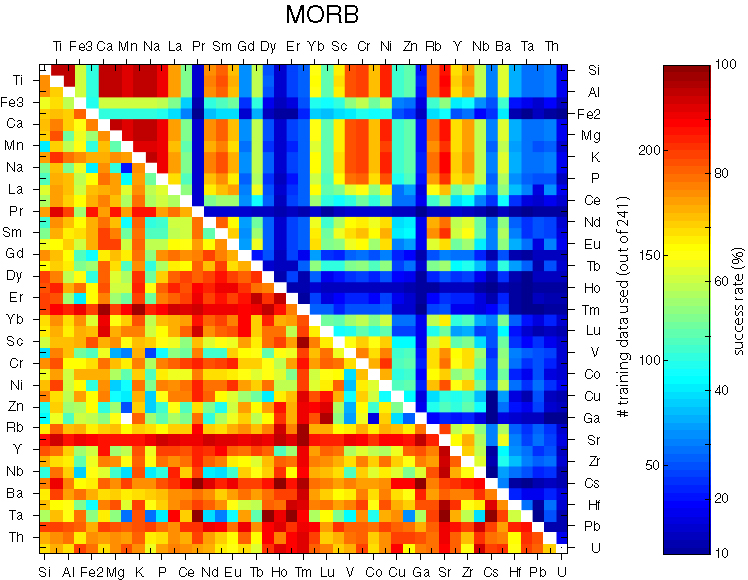
\includegraphics[width=300]{figures/xPlotTrace2_linear_MORB.jpg}\\
  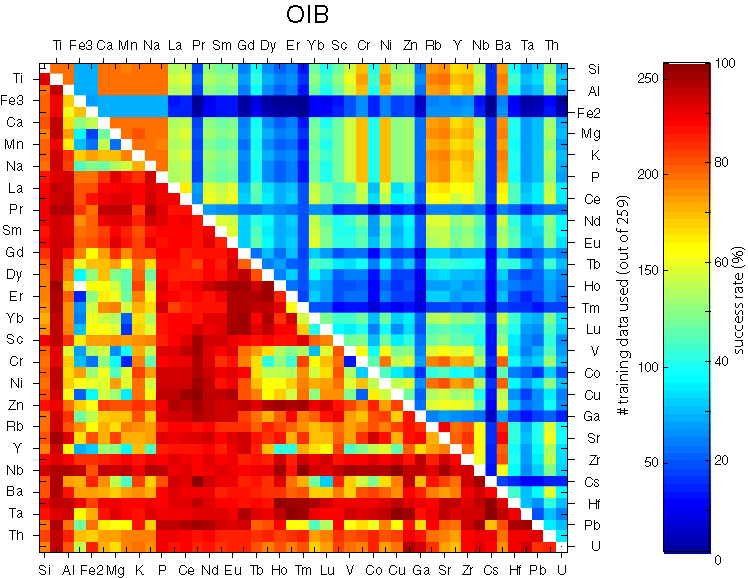
\includegraphics[width=300]{figures/xPlotTrace2_linear_OIB.jpg}
  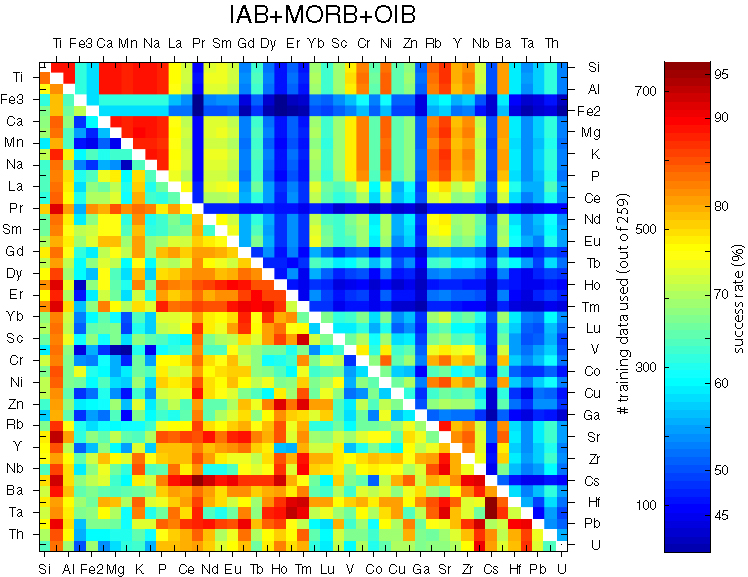
\includegraphics[width=300]{figures/xPlotTrace2_linear_err.jpg}
  \caption[Matrices   showing   the  performance   of   all  possible   bivariate
discriminant analyses using combinations of 45 elements]
{Matrices   showing   the  performance   of   all  possible   bivariate linear
discriminant analyses using combinations of 45 elements.}
  \label{fig:trace2lin}
\end{figure}

\begin{figure}[htbp]
  \centering
  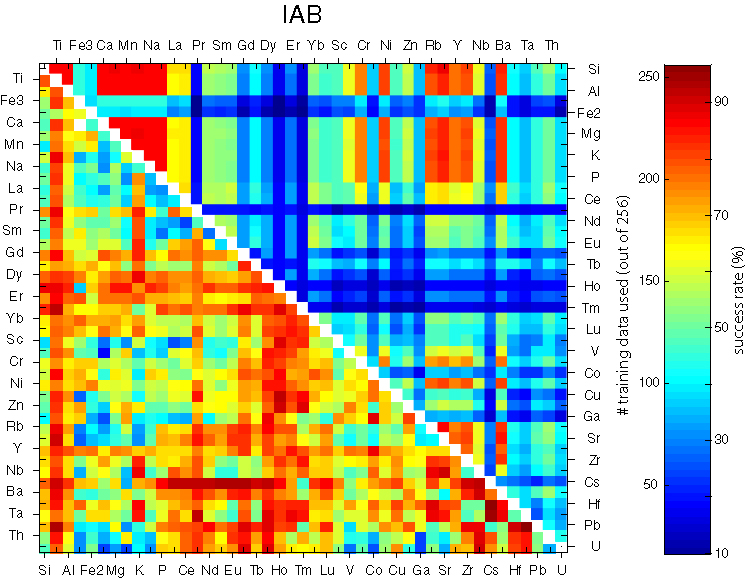
\includegraphics[width=300]{figures/xPlotTrace2_quadratic_IAB.jpg}
  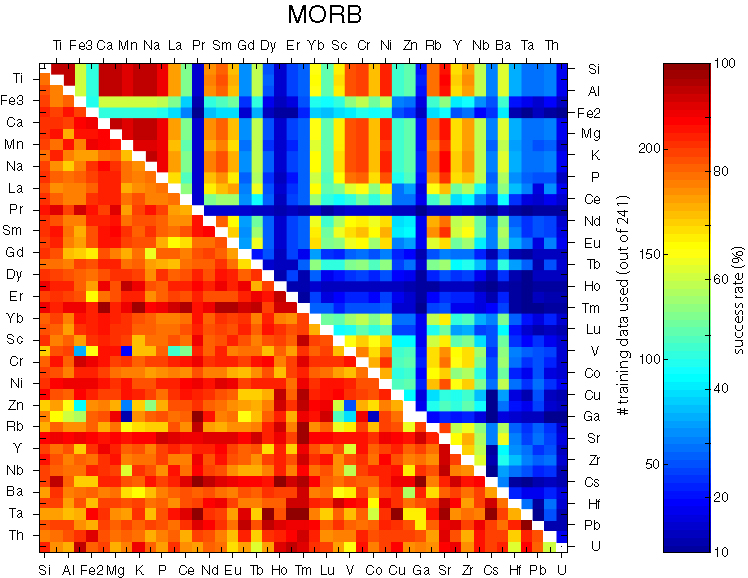
\includegraphics[width=300]{figures/xPlotTrace2_quadratic_MORB.jpg}\\
  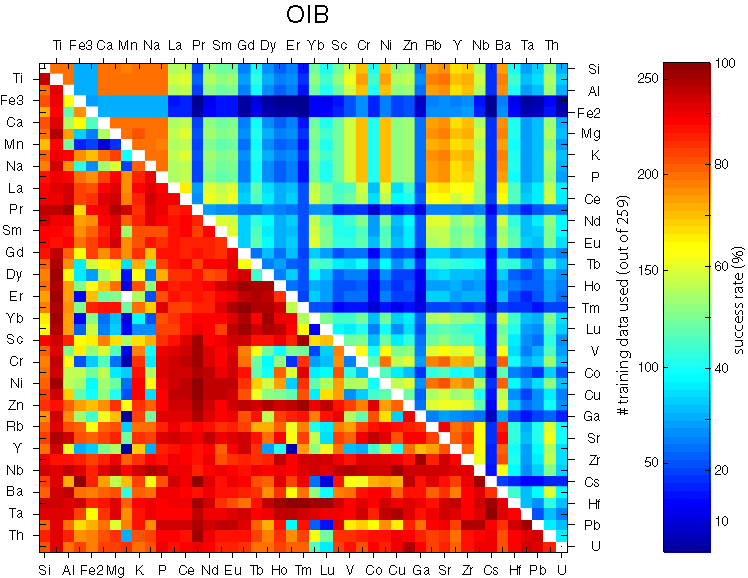
\includegraphics[width=300]{figures/xPlotTrace2_quadratic_OIB.jpg}
  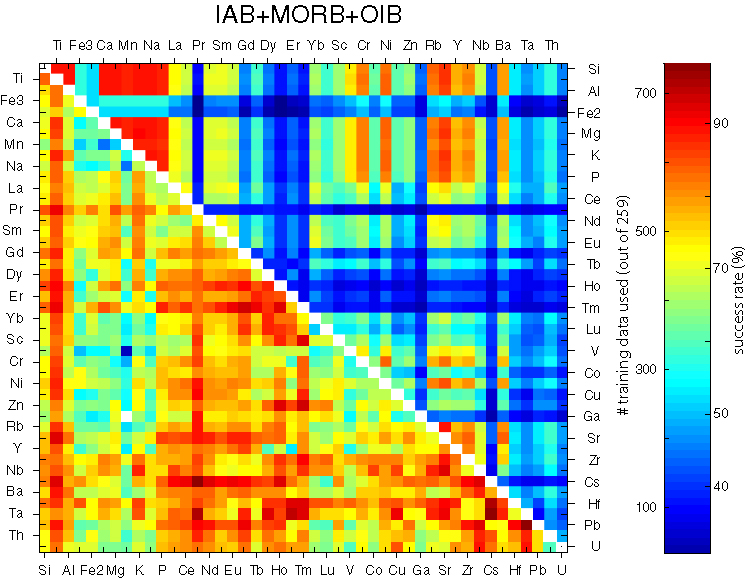
\includegraphics[width=300]{figures/xPlotTrace2_quadratic_err.jpg}
  \caption[Same  as Figure  \ref{fig:trace2lin}, but  for  quadratic discriminant analysis]
{Same  as Figure  \ref{fig:trace2lin}, but  for  quadratic discriminant analysis.}
  \label{fig:trace2quad}
\end{figure}

\clearpage

\begin{figure}[htbp]
  \centering
  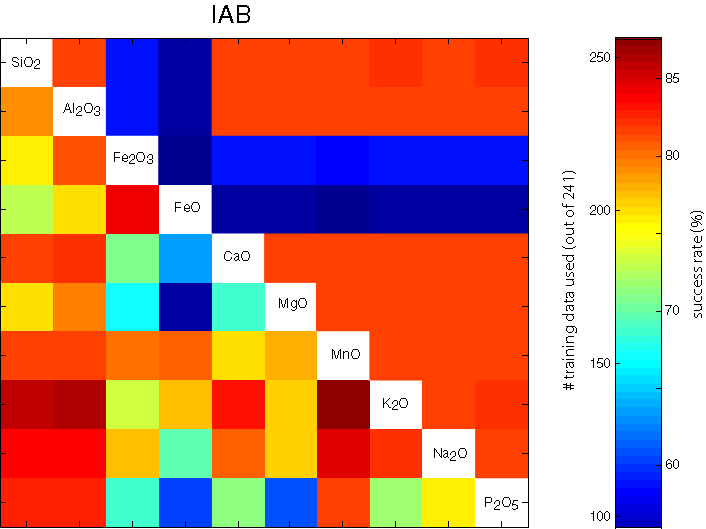
\includegraphics[width=300]{figures/xPlotMajor3Ti_linear_IAB.jpg}
  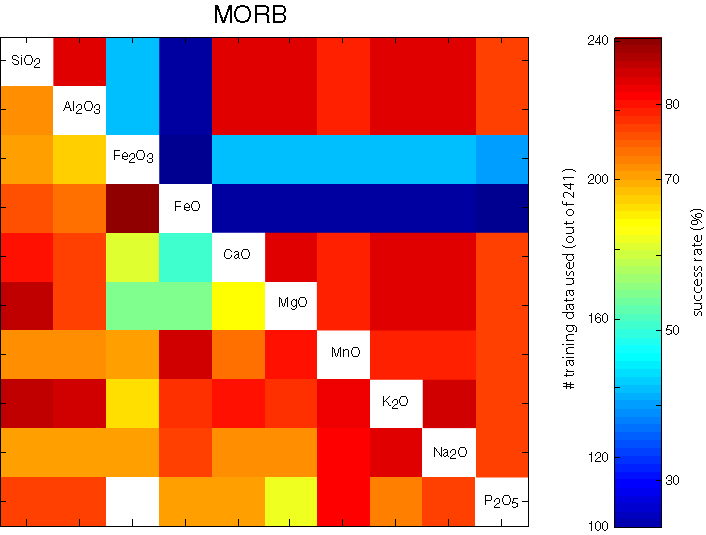
\includegraphics[width=300]{figures/xPlotMajor3Ti_linear_MORB.jpg}\\
  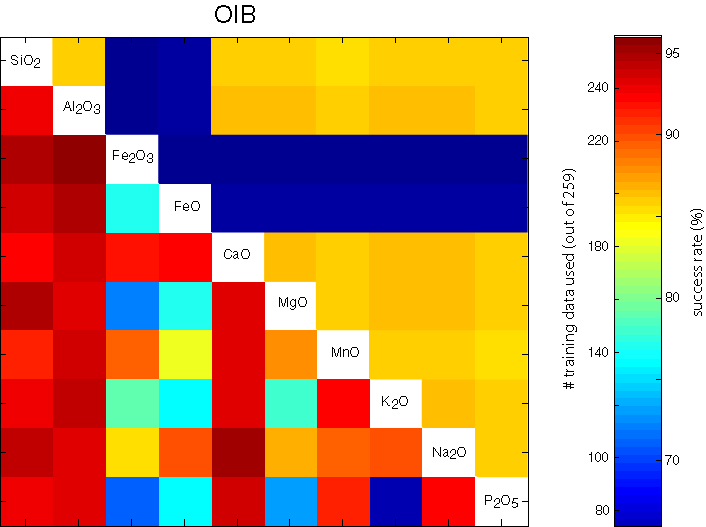
\includegraphics[width=300]{figures/xPlotMajor3Ti_linear_OIB.jpg}
  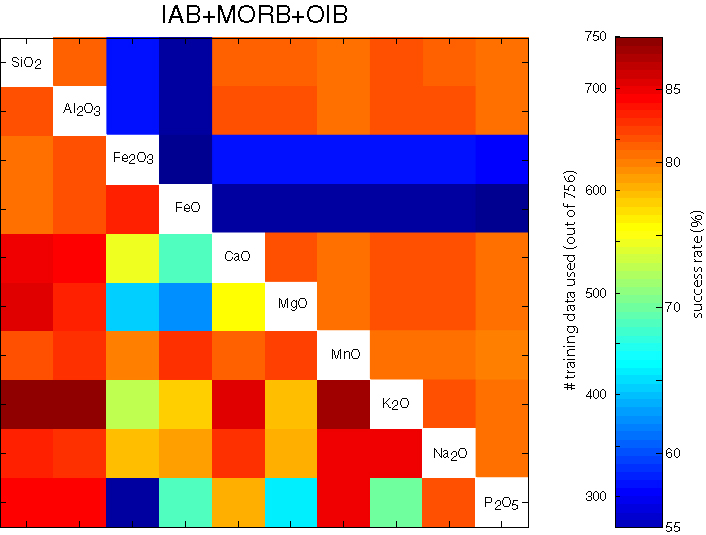
\includegraphics[width=300]{figures/xPlotMajor3Ti_linear_err.jpg}
  \caption[Performance  analysis of  all possible  ternary  discriminant analyses
 using TiO$_2$ and other major element oxides]
{Performance  analysis of  all possible  ternary  discriminant analyses
 using TiO$_2$ and other major element oxides.}
  \label{fig:major3lin}
\end{figure}

\begin{figure}[htbp]
  \centering
  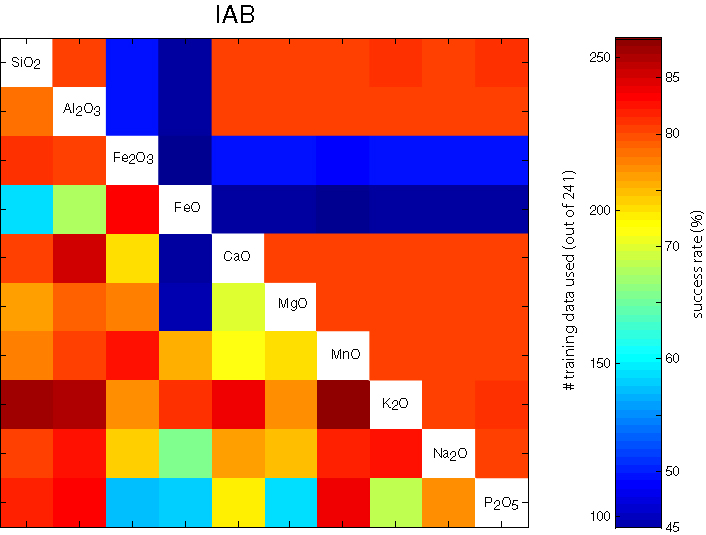
\includegraphics[width=300]{figures/xPlotMajor3Ti_quadratic_IAB.jpg}
  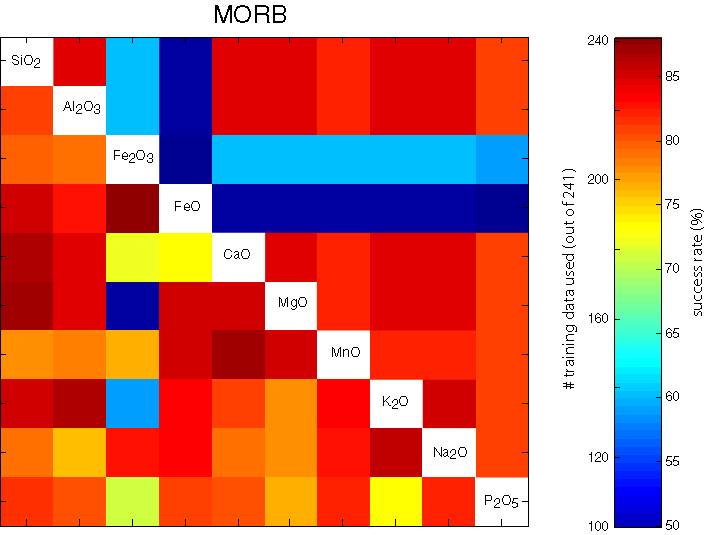
\includegraphics[width=300]{figures/xPlotMajor3Ti_quadratic_MORB.jpg}\\
  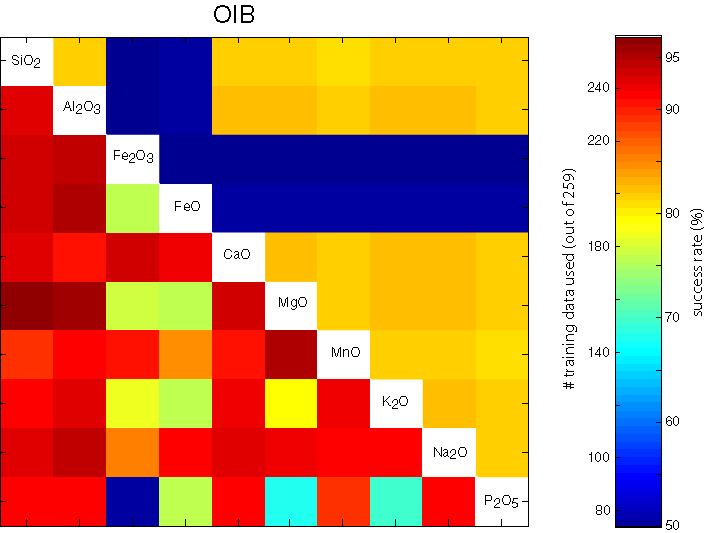
\includegraphics[width=300]{figures/xPlotMajor3Ti_quadratic_OIB.jpg}
  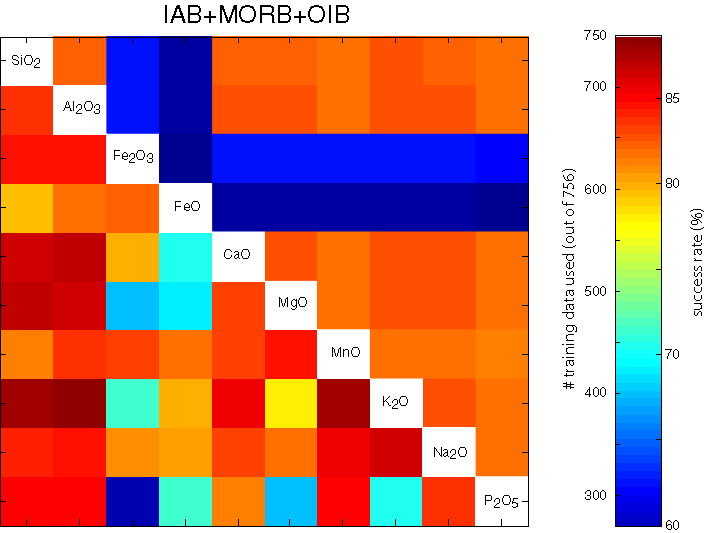
\includegraphics[width=300]{figures/xPlotMajor3Ti_quadratic_err.jpg}
  \caption[Same as  Figure \ref{fig:major3lin}, but  using quadratic discriminant analysis]
{Same as  Figure \ref{fig:major3lin}, but  using quadratic discriminant analysis.}
  \label{fig:major3quad}
\end{figure}

\begin{figure}[htbp]
  \centering
  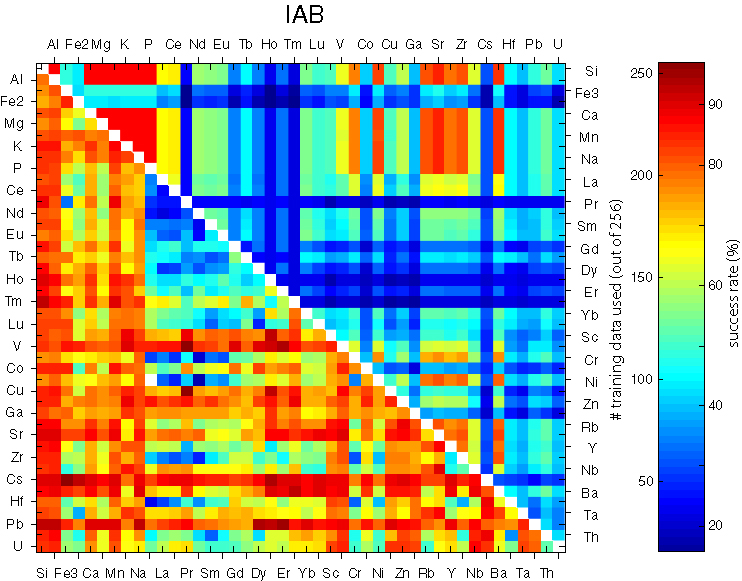
\includegraphics[width=300]{figures/xPlotTrace3Ti_linear_IAB.jpg}
  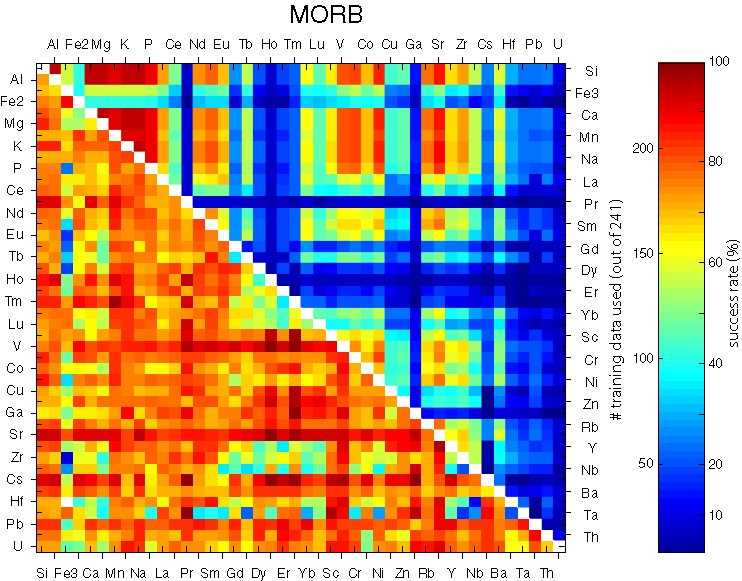
\includegraphics[width=300]{figures/xPlotTrace3Ti_linear_MORB.jpg}\\
  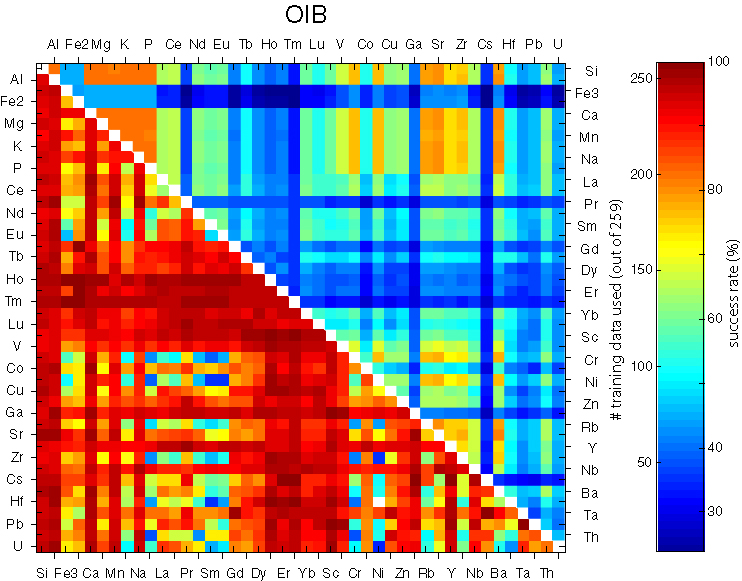
\includegraphics[width=300]{figures/xPlotTrace3Ti_linear_OIB.jpg}
  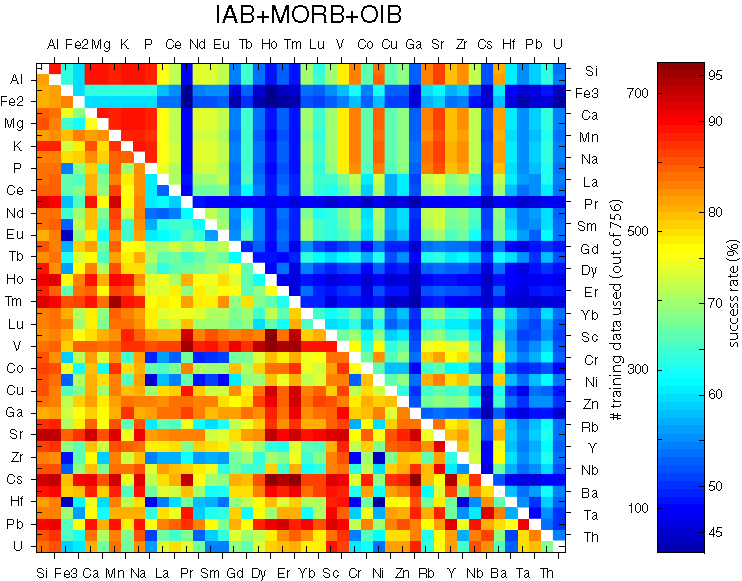
\includegraphics[width=300]{figures/xPlotTrace3Ti_linear_err.jpg}
  \caption[Performance  analysis of  all possible  ternary  discriminant analyses
using Ti and other elements]
{Performance  analysis of  all possible  ternary  discriminant analyses
using Ti and two of 45 other elements.}
  \label{fig:trace3lin}
\end{figure}

\begin{figure}[htbp]
  \centering
  \includegraphics[width=300]{figures/xPlotTrace3Ti_quadratic_IAB.jpg}
  \includegraphics[width=300]{figures/xPlotTrace3Ti_quadratic_MORB.jpg}\\
  \includegraphics[width=300]{figures/xPlotTrace3Ti_quadratic_OIB.jpg}
  \includegraphics[width=300]{figures/xPlotTrace3Ti_quadratic_err.jpg}
  \caption[Same as  Figure \ref{fig:trace3lin}, but  using quadratic discriminant analysis]
{Same as  Figure \ref{fig:trace3lin}, but  using quadratic discriminant analysis.}
  \label{fig:trace3quad}
\end{figure}

\clearpage

\begin{figure}[htbp]
  \centering
  \includegraphics[width=600]{figures/Si_Ti_Sr_lin.jpg}
  \caption[Best ternary linear discriminant analysis (using Si, Ti, and Sr)]{
The best ternary linear discriminant analysis, using Si, Ti, and Sr.}
  \label{fig:Si_Ti_Sr_lin}
\end{figure}

\begin{figure}[htbp]
  \centering
  \includegraphics[width=600]{figures/Eu_Lu_Sr_lin.jpg}
  \caption[Linear discriminant analysis using Eu, Lu, and Sr]
{Linear discriminant analysis using Eu, Lu, and Sr.}
  \label{fig:Eu_Lu_Sr_lin}
\end{figure}

\begin{figure}[htbp]
  \centering
  \includegraphics[width=600]{figures/V_Ti_Sc_lin.jpg}
  \caption[Linear discriminant analysis using Ti, V and Sc]
{The   best  performing  linear   discriminant  analysis   using  only
incompatible elements (Ti, V and Sc).}
  \label{fig:V_Ti_Sc_lin}
\end{figure}

\clearpage

\begin{figure}[htbp]
  \centering
  \includegraphics[width=600]{figures/Na_Nb_Sr_quad.jpg}
  \caption[Quadratic discriminant analysis using Na, Nb and Sr]
{The best performing quadratic discriminant analysis, using Na, Nb and
Sr.}
  \label{fig:Na_Nb_Sr_quad}
\end{figure}

\begin{figure}[htbp]
  \centering
  \includegraphics[width=600]{figures/V_Ti_Sm_quad.jpg}
  \caption[Quadratic discriminant analysis using Ti, V and Sm]
{The  best  performing  quadratic  discriminant  analysis  using  only
incompatible elements (Ti, V and Sm).}
  \label{fig:V_Ti_Sm_quad}
\end{figure}

\begin{figure}[htbp]
  \centering
  \includegraphics[width=500]{figures/biasVariance.jpg}
  \caption[Illustration of the bias-variance tradeoff in a regression context]
{Illustration of  the bias-variance tradeoff in  a regression context.
The thick gray  line is the true model (Y =  X$^4$). The white circles
are  50 samples with  random normal  errors.  The  dashed line  is the
interpolator,  which  is one  of  infinitely  many  functions that  go
through all the datapoints and,  thus, have zero bias. The solid black
line is  a linear regression model,  which has a large  bias but small
variance. In this case, the fourth order polynomial (blue) is the best
predictor of  future behavior.  Although  it has larger bias  than the
50th order polynomial  (red) and larger variance than  the first order
polynomial (straight black line),  it minimizes the mean squared error
(MSE = variance + bias$^2$).}
  \label{fig:biasVariance}
\end{figure}

\begin{figure}[htbp]
  \centering
a.  \includegraphics[width=300]{figures/Shervais.jpg}\\
b.  \includegraphics[width=300]{figures/log_Ti_V_lin.jpg}
c.  \includegraphics[width=300]{figures/log_Ti_V_q.jpg}
d.  \includegraphics[width=300]{figures/test_Ti_V_lin.jpg}
e.  \includegraphics[width=300]{figures/test_Ti_V_q.jpg}
  \caption[The test data plotted on various versions of the Ti-V diagram]
{The test data (116/182 used)  plotted on various versions of the Ti-V
diagram with: a. the  original decision boundaries of Shervais (1982),
drawn by  eye; b.   LDA on the  logratio-plot, with anchor  points 1-4
given in Table \ref{tab:anchors}; c.  QDA on the logratio-plot, d. the
same  LDA  as  in  subplot  b.,  but this  time  mapped  back  to  the
``traditional''  compositional  data space;  e.   the  QDA of  subplot
c.  mapped  back  to  Ti-V  space.  An error  analysis  of  these  and
subsequent   diagrams  is   given  in   Tables   \ref{tab:errEst}  and
\ref{tab:comparison}.}
  \label{fig:log_Ti_V}
\end{figure}

\begin{figure}[htbp]
  \centering
a.  \includegraphics[width=300]{figures/PearceTiZr.jpg}\\
b.  \includegraphics[width=300]{figures/log_Ti_Zr_lin.jpg}
c.  \includegraphics[width=300]{figures/log_Ti_Zr_q.jpg}
d.  \includegraphics[width=300]{figures/test_Ti_Zr_lin.jpg}
e.  \includegraphics[width=300]{figures/test_Ti_Zr_q.jpg}
  \caption[The test data plotted on the Ti-Zr diagram]
{The test data (89/182 used) plotted on the Ti-Zr diagram with: a. the
original  decision boundaries  of Pearce  and Cann  (1973); b-e  as in
Figure \ref{fig:log_Ti_V}.}
  \label{fig:log_Ti_Zr}
\end{figure}

\begin{figure}[htbp]
  \centering
a.  \includegraphics[width=300]{figures/PearceTiZrY.jpg}\\
b.  \includegraphics[width=300]{figures/log_Ti_Zr_Y_lin.jpg}
c.  \includegraphics[width=300]{figures/log_Ti_Zr_Y_q.jpg}
d.  \includegraphics[width=300]{figures/test_Ti_Zr_Y_lin.jpg}
e.  \includegraphics[width=300]{figures/test_Ti_Zr_Y_q.jpg}
  \caption[The test data plotted on the Ti-Zr-Y diagram]{
The  test data  (85/182 used)  plotted  on the  Ti-Zr-Y diagram  with:
a. the original decision boundaries  of Pearce and Cann (1973); b-e as
in Figure \ref{fig:log_Ti_V}.}
  \label{fig:log_Ti_Zr_Y}
\end{figure}

\begin{figure}[htbp]
  \centering
a.  \includegraphics[width=300]{figures/Meschede.jpg}\\
b.  \includegraphics[width=300]{figures/log_Nb_Zr_Y_lin.jpg}
c.  \includegraphics[width=300]{figures/log_Nb_Zr_Y_q.jpg}
d.  \includegraphics[width=300]{figures/test_Nb_Zr_Y_lin.jpg}
e.  \includegraphics[width=300]{figures/test_Nb_Zr_Y_q.jpg}
  \caption[The test data plotted on the Nb-Zr-Y diagram]
{The test data  (58/182 used) plotted on the  Nb-Zr-Y diagram with: a.
the original decision boundaries of  Meschede (1986); b-e as in Figure
\ref{fig:log_Ti_V}.}
  \label{fig:log_Nb_Zr_Y}
\end{figure}

\begin{figure}[htbp]
  \centering
a.  \includegraphics[width=300]{figures/Wood.jpg}\\
b.  \includegraphics[width=300]{figures/log_Th_Ta_Hf_lin.jpg}
c.  \includegraphics[width=300]{figures/log_Th_Ta_Hf_q.jpg}
d.  \includegraphics[width=300]{figures/test_Th_Ta_Hf_lin.jpg}
e.  \includegraphics[width=300]{figures/test_Th_Ta_Hf_q.jpg}
  \caption[The test data plotted on the Th-Ta-Hf diagram]
{The test  data (36/182 used, but  no MORBs!) plotted  on the Th-Ta-Hf
diagram with: a. the original  decision boundaries of Wood (1980); b-e
as in Figure \ref{fig:log_Ti_V}.}
  \label{fig:log_Th_Ta_Hf}
\end{figure}

\begin{figure}[htbp]
  \centering
a.  \includegraphics[width=300]{figures/log_Si_Ti_Sr_lin.jpg}
b.  \includegraphics[width=300]{figures/test_Si_Ti_Sr_lin.jpg}
  \caption[The test data plotted on the Si-Ti-Sr diagram]
{The  test data  (164/182 used)  plotted on  the Si-Ti-Sr  LDA diagram
with:  a.   the  decision  boundaries  and anchor  points  (see  Table
\ref{tab:anchors})  in log-ratio  space; b.   the  decision boundaries
mapped back to the simplex.}
  \label{fig:log_Si_Ti_Sr}
\end{figure}

\begin{figure}[htbp]
  \centering
a.  \includegraphics[width=300]{figures/log_Eu_Lu_Sr_lin.jpg}
b.  \includegraphics[width=300]{figures/test_Eu_Lu_Sr_lin.jpg}
  \caption[The test data plotted on the Eu-Lu-Sr diagram]
{The test data (103/182 used)  plotted on the Eu-Lu-Sr LDA diagram;  a
\& b as in Figure \ref{fig:log_Si_Ti_Sr}.}
  \label{fig:log_Eu_Lu_Sr}
\end{figure}

\begin{figure}[htbp]
  \centering
a.  \includegraphics[width=300]{figures/log_V_Ti_Sc_lin.jpg}
b.  \includegraphics[width=300]{figures/test_V_Ti_Sc_lin.jpg}
  \caption[The test data plotted on the Ti-V-Sc diagram]
{The test data (72/182 used) plotted on the Ti-V-Sc LDA diagram;  a \&
b as in Figure \ref{fig:log_Si_Ti_Sr}.}
  \label{fig:log_V_Ti_Sc}
\end{figure}

\begin{figure}[htbp]
  \centering
a.  \includegraphics[width=300]{figures/log_Na_Nb_Sr_q.jpg}
b.  \includegraphics[width=300]{figures/test_Na_Nb_Sr_q.jpg}
  \caption[The test data plotted on the Na-Nb-Sr diagram]
{The test data (61/182 used) plotted on the Na-Nb-Sr QDA diagram with:
a.   the decision  boundaries in  log-ratio space;  b. mapped  back to
$\Delta_2$.}
  \label{fig:log_Na_Nb_Sr}
\end{figure}

\begin{figure}[htbp]
  \centering
a.  \includegraphics[width=300]{figures/log_Ti_V_Sm_q.jpg}
b.  \includegraphics[width=300]{figures/test_Ti_V_Sm_q.jpg}
  \caption[The test data plotted on the Ti-V-Sm diagram]
{The test data (85/182 used) plotted on the Ti-V-Sm QDA diagram;  a \&
b as in Figure \ref{fig:log_Na_Nb_Sr}.}
  \label{fig:log_Ti_V_Sm}
\end{figure}



\end{document}
